% !TeX TXS-program:compile = txs:///pdflatex/[--shell-escape]

%Hierarchie der Überschriften
%\section{}
%\subsection{}
%\subsubsection{}
%\paragraph{}
%\minisec{} Kann man für kleine Überschriften ohne Nummerierung verwenden

\pdfminorversion=7

%% ========== TITLE INFORMATION ==========
\newcommand{\thesistype}{DA} 
\newcommand{\thesislanguage}{de-AT}
\newcommand{\thesistitle}{Entwicklung einer Anzeigelösung für Lüftungsanlagen auf Basis des "Modbus"-Protokolls}
\newcommand{\fenkart}{Lukas Fenkart}
\newcommand{\mangeng}{Luca Jerome Mangeng}
\newcommand{\pezze}{Damiano Pezzè}
\newcommand{\schneider}{Martin Schneider}

\documentclass[12pt,twoside=false, a4paper]{scrreprt}

\usepackage{TUWBUIDADISS}

\raggedbottom 
%% prevents the expansion of the text till the end of the page (if you like)
%\setcapindent{0em} %% influences captions layout
%%
%% ========== Key Words ==========
\begin{filecontents}[overwrite]{\jobname.xmpdata}
\Language{\thesislanguage}
\Title{\thesistitle}
\Keywords{Diplomarbeit\sep \sep LaTeX}
\end{filecontents}

%% use biblatex and biber for bibliography
\usepackage[style=numeric-comp,backend=biber,maxcitenames=2]{biblatex}
\ExecuteBibliographyOptions{%
  giveninits=false,maxbibnames=99}%
\DefineBibliographyStrings{ngerman}{andothers={et\;al\adddot},
urlseen = {Zugriff am}}
\addbibresource{Literatur.bib}

%% ===== additional packages to the ones already loaded ==============
\usepackage{acro}
%\ac{Kuerzel} wird der Befehl \ac{Kuerzel} das erste Mal verwendet, erhält man die Langform des Ausdrucks und zusätzlich die geklammerte Kurzform. Wird der Befehl danach wieder mit dem gleichen Kürzel, erhält man die Kurzform dann aber ohne Klammern.
%\acl{Kuerzel} schreibt die Langform des Ausdrucks.
%\acs{Kuerzel} schreibt die Kurzform.
%\aclp{Kuerzel} schreibt die Langform des Plurals des Ausdrucks.
%\acsp{Kuerzel}schreibt die Kurzform des Plurals. 
%\acf{Kuerzel} verhält sich wie \ac{Kuerzel} Befehl, wenn er das erste Mal aufgerufen wurde. Unabhängig davon, wie oft das Kürzel bereits aufgerufen wurde, wird bei der Verwendung von \acf{Kuerzel} die ausgeschriebene Langform des Ausdrucks und die geklammerte Abkürzung gesetzt.

\DeclareAcronym{obv}{
short = {\"obv},
long  = {Österreichische Bautechnikvereinigung},
}

\DeclareAcronym{dt}{
short = {dt.},
long  = {deutsch},
}

\DeclareAcronym{engl}{
	short = {engl.},
	long  = {englisch},
}

\DeclareAcronym{python}{
	short = {Python},
	long  = {},
}

\DeclareAcronym{abbv}{
short = {ABBV},
long  = {Ablösungsbeträge-Berechnungsverordnung},
short-plural = {s},
long-plural = {en},
}

\DeclareAcronym{lzk}{
short = {LZK},
long  = {Lebenszykluskosten},
extra = {[\officialeuro{}]},
}

\DeclareAcronym{rlt}{
	short = RLT,
	long  = raumlufttechnische,
	short-plural = s,
	long-plural = n,
}

\DeclareAcronym{rltanlage}{
	short = RLT Anlage,
	long  = raumlufttechnische Anlage,
	short-plural = n,
	long-plural-form = raumlufttechnische Anlagen,
}

\DeclareAcronym{rltanlagen}{
	short = RLT Anlagen,
	long  = raumlufttechnische Anlagen,
}

\DeclareAcronym{gui}{
	short = GUI,
	long  = Grafische Benutzeroberfläche,
	short-plural = s,
	long-plural = n,
}

\DeclareAcronym{htl}{
	short = HTL,
	long  = Höhere Technische Bundeslehr- und Versuchsanstalt,
}

\DeclareAcronym{json}{
	short = \gls{gls_json},
	long  = JavaScript Object Notation,
}

\DeclareAcronym{csv}{
	short = \gls{gls_csv},
	long  = Comma-Separated Values,
}

\DeclareAcronym{rfc}{
	short = RFC,
	long  = Request for Comments,
}

\DeclareAcronym{mime}{
	short = MIME-Type,
	long  = Internet Media Type,
}

\DeclareAcronym{crlf}{
	short = CRLF,
	long  = Carriage Return Line feed,
}

\DeclareAcronym{pdu}{
	short = PDU,
	long = Protocol Data Unit,
}

\DeclareAcronym{adu}{
	short = ADU,
	long = Application Data Unit,
}

\DeclareAcronym{tcp}{
	short = TCP,
	long = Transmission Control Protocol,
}

\DeclareAcronym{rtu}{
	short = RTU,
	long = Remote Terminal Unit, 
}

\DeclareAcronym{ascii}{
short = ASCII,
long = American Standard Code for Information Interchange, 
}

\DeclareAcronym{io}{
	short = I/O System,
	long = Input/Output System, 
}

\DeclareAcronym{rltanzeige}{
	short = RLT Anzeige,
	long = Raumlufttechnische Anzeige,
}

\DeclareAcronym{crc}{
short = CRC,
long = Cyclical Redundancy Checking, 
}

\DeclareAcronym{lrc}{
short = LRC,
long = Longitudinal Redundancy Checking, 
}

\DeclareAcronym{xml}{
	short = XML,
	long = Extensible Markup Language,
}



\usepackage{pdflscape}
\usepackage{longtable}

%% Einstellungen für Zeilenumbrüche von Weblinks im url-Paket
\setcounter{biburllcpenalty}{9000}% Kleinbuchstaben
\setcounter{biburlucpenalty}{9000}% Großbuchstaben
%% Quelle: https://texwelt.de/fragen/7008/zeilenumbruche-in-bibliografielinks

%% ===== additional settings =============
\setcounter{secnumdepth}{3}
\sisetup{output-decimal-marker = {,},
range-phrase = --,
group-separator = {~},
per-mode = symbol, 
list-final-separator={ und }}

%Damit bei untrennbaren Wörtern nicht über den Rand geschrieben wird
\setlength{\emergencystretch}{3em}

\graphicspath{{Bilder/}}

%% examples for useful shortcuts in German
\newcommand{\zB}{\mbox{z.\,B.}\xspace}
\newcommand{\dt}{\mbox{\acs{dt}}\xspace}
\newcommand{\engl}{\mbox{\acs{engl}}\xspace}
\newcommand{\bzw}{\mbox{bzw.}\xspace}
\newcommand{\ggf}{\mbox{ggf.}\xspace}
\newcommand{\Name}[1]{\textsc{#1}}

\newcommand{\vKTxv}{\mathbf{v}_1^T\tilde{\mathbf{K}}_{T},_{\xi}\mathbf{v}_1}
\newcommand{\vKTxxv}{\mathbf{v}_1^T\tilde{\mathbf{K}}_{T},_{\xi\xi}\mathbf{v}_1}

% activate for double space between the lines (correction mode) 
%\doublespacing

\makeglossaries
%\loadglsentries{Glossar}
% Anleitung:
% https://en.wikibooks.org/wiki/LaTeX/Glossary

% BEFEHLE FÜR GLOSSAREINTRÄGE.

% \gls{<label>} 
% prints the term associated with <label> passed as its argument.

% \glspl{<label>}
% prints the plural of the defined term.

% \Gls{<label>}
% prints the singular form with the first character converted to upper case.

% \Glspl{<label>}
% prints the plural form with first character converted to upper case.

% BEFEHLE FÜR ACRONYME:

% \acrlong{<label>}
% long version of an acronym

% \acrfull{<label>}
% print the long version of an acronym and the abbreviation

% \acrshort{<label>}
% print the abbreviation


%Beispiele:
\newacronym{vm}{VM}{Virtuelle Maschine}

\newglossaryentry{latex}
{
	name=latex,
	description={LaTeX (short for Lamport TeX) is a document preparation system. The user has to think about only the content to put in the document and the software will take care of the formatting. }
}

\newglossaryentry{glsy}
{
	name=glossary,
	description={Acronyms and terms which are generally unknown or new to common readers.}
}

\newglossaryentry{gpio}
{
	name=GPIO,
	description={Als GPIO (Kurzform für General-Purpose Input-Output) bezeichnet man die Pins auf einem Mikrocontroller. Diese können elektrische Signale senden und empfangen, sind aber nicht für einen spezifischen Gebrauch entwickelt}
}

\newglossaryentry{hdmi}
{
	name=HDMI,
	description={HDMI (Kurzform für High-Definition Multimedia Interface) ist eine Multimedia-Schnittstelle für die Übertragung von Audio- und Videosignalen}
}

\newglossaryentry{osi}
{
	name=OSI,
	description={OSI (Open System Interconnection) ist die Internationale Organisation für Normung, als Grundlage für die Bildung von offenen Kommunikationsstandards}
}

\newglossaryentry{parity}
{
	name=Parität,
	description={Gibt an ob eine Zahl gerade oder ungerade ist, also ob sie ohne Rest durch 2 teilbar ist \cite{Parity_Mathematik:o.J.}}
}

\newglossaryentry{gls_tcp}
{
	name=TCP,
	description={TCP (Transmission Control Protocol) ist ein Standard, der definiert, wie eine Netzwerkkonversation aufgebaut und aufrechterhalten wird, über die Anwendungen Daten austauschen können}
}

\newglossaryentry{gls_rtu}
{
	name=RTU,
	description={\ref{modbus_uebertragungsarten} \nameref{modbus_uebertragungsarten}}
}

\newglossaryentry{gls_ascii}
{
	name=ASCII,
	description={Der American Standard Code for Information Interchange ist ein Zeichensatz, der mit 7-Bits die meisten Zeichen einer US-Amerikanischen Computertastatur darstellen kann \cite{seo_kueche_ascii:o.J.}}
}

\newglossaryentry{client}
{
	name=Client,
	description={\ref{begriffserklaerung} \nameref{begriffserklaerung}}
}

\newglossaryentry{server}
{
	name=Server,
	description={\ref{begriffserklaerung} \nameref{begriffserklaerung}}
}

\newglossaryentry{gls_pdu}
{
	name=PDU,
	description={\ref{modbus_funktionsweise} \nameref{modbus_funktionsweise}}
}

\newglossaryentry{gls_adu}
{
	name=ADU,
	description={\ref{modbus_funktionsweise} \nameref{modbus_funktionsweise}}
}

\newglossaryentry{xor}
{
	name=XOR,
	description={XOR ist eine binäre Rechenoperation, bei der zwei Bits miteinander verglichen werden. Das resultierende Bit ist 1, wenn genau eines der verglichenen Bits 1 ist}
}

\newglossaryentry{gls_crc}
{
	name=CRC,
	description={\ref{modbus_uebertragungsarten} \nameref{modbus_uebertragungsarten}}
}

\newglossaryentry{gls_lrc}
{
	name=LRC,
	description={\ref{modbus_uebertragungsarten} \nameref{modbus_uebertragungsarten}}
}

\newglossaryentry{cr}
{
	name=CR,
	description={ASCII Kontrollzeichen. Bewegt den Cursor an den Anfang der Zeile \cite{Mozilla_CRLF:2023}}
}

\newglossaryentry{lf}
{
	name=LF,
	description={ASCII Kontrollzeichen. Bewegt den Cursor eine Zeile nach unten \cite{Mozilla_CRLF:2023}}
}

\newglossaryentry{zuluft}
{
	name=Zuluft,
	description={Bei der Zuluft handelt es sich um die Luft welche im Lüftungsgerät schon behandelt (gefiltert) wurde}
}

\newglossaryentry{abluft}
{
	name=Abluft,
	description={Bei der Abluft handelt es sich um die Luft welche aus dem Innenraum (Gebäude) abgesaugt wird}
}

\newglossaryentry{fortluft}
{
	name=Fortluft,
	description={Bei der Fortluft handelt es sich um die Luft welche aus dem Gebäude und der Lüftungsanlage nach draußen in die Umwelt geleitet wird}
}

\newglossaryentry{aussenluft}
{
	name=Außenluft,
	description={Bei der Außenluft handelt es sich um die Luft aus der Umwelt, welche noch unbehandelt (nicht gefiltert) in die Lüftungsanlage eingesaugt wird}
}

\newglossaryentry{tdot}
{
	name=TdoT,
	description={Der Tdot ist der Tag der offenen Tür der HTL Dornbirn. An diesem Tag wurde ein Lüftungsgerät der Firma Bösch ausgestellt inkl. RLT Anzeige}
}

\newglossaryentry{qbm}
{
	name=QBM,
	description={Eine Serie von Luftdruckfühlern der Marke Siemens. Im Falle der Diplomarbeit ist das Modell QBM9711 in Verwendung, welches über eine I/O-Erweiterung verfügt, an die externe Sensorik angeschlossen werden kann bzw. mit der externe Geräte gesteuert werden können}
}

\glstoctrue %Glossar im Inhaltsverzeichnis anzeigen

\begin{document}       %% start of the document
\maketitle             %% places the title with above information

%\cleardoublepage
\selectlanguage{ngerman} 
\pagestyle{scrheadings} 

%\addchap{\textit{Placeholder Eidesstaatliche Erklärung}}
\addchap{Eidesstattliche Erklärung}

\vspace{30pt}

\begin{center}
    \textbf{\LARGE Entwicklung einer Anzeigelösung für Lüftungsanlagen auf Basis des "Modbus"-Protokolls}
\end{center}

\vspace{30pt}

\noindent Die Verfasser erklären an Eides statt, dass sie die vorliegende Diplomarbeit selbstständig und ohne fremde Hilfe verfasst, keine anderen als die angegebenen Quellen und Hilfsmittel benutzt und die den benutzten Quellen wörtlich und inhaltlich entnommenen Stellen als solche erkenntlich gemacht haben.

\vfill

\noindent
\begin{minipage}[t]{0.35\textwidth}
\centering
\underline{\hspace{5cm}} \\
\vspace{-0.4\baselineskip}
Dornbirn, am \\
\underline{\hspace{5cm}} \\
\vspace{-0.4\baselineskip}
Dornbirn, am \\
\underline{\hspace{5cm}} \\
\vspace{-0.4\baselineskip}
Dornbirn, am \\
\underline{\hspace{5cm}} \\
\vspace{-0.4\baselineskip}
Dornbirn, am \\
\end{minipage}

\hfill

\begin{minipage}[t]{0.55\textwidth}
\centering
\underline{\hspace{7cm}} \\
\vspace{-0.4\baselineskip}
\fenkart \\
\underline{\hspace{7cm}} \\
\vspace{-0.4\baselineskip}
\mangeng \\
\underline{\hspace{7cm}} \\
\vspace{-0.4\baselineskip}
\pezze \\
\underline{\hspace{7cm}} \\
\vspace{-0.4\baselineskip}
\schneider \\
\end{minipage}


% Vorwort übersetzt
\addchap{Abstract (DE)}


\selectlanguage{english} 
\addchap{Abstract (EN)}














\selectlanguage{ngerman} 

% Persönlich
\addchap{Vorwort}
\noindent ...

\tableofcontents

% Persönlich
\addchap{Danksagung}
An dieser Stelle möchten wir uns bei allen Akteuren bedanken, die uns mit Rat und Tat zur Seite standen, uns motiviert oder finanziell unterstützt haben.

Zuerst möchten wir uns bei der Walter Bösch GmbH \& Co. KG bedanken, die uns diese Diplomarbeit ermöglicht haben und auch die Kosten der zur Erstellung notwendigen Hardware trugen. Besonders aber danken wir unserem Betreuer auf Firmenseite Simon Köldorfer, der uns bei Fragen und Problemen half, sich um die Beschaffung der Teile (\zB 3D gedrucktes Gehäuse) und unseren außergewöhnlichen Auftritt am Tag der offenen Tür ermöglichte. Außerdem gilt dieser Dank auch Christoph Grabher-Meyer, der uns ebenfalls immer wieder ausgeholfen hat.

Ein herzlicher Dank geht weiters an unsere Schule, die HTL Dornbirn, für die lehrreichen Jahre, die bereitgestellten Ressourcen und die unterstützende Lernumgebung. Besonders möchten wir uns bei unserem Betreuungslehrer Klaus Battlogg für die wertvollen Ratschläge beim organisatorischen und schriftlichen Teil und für das Korrekturlesen dieser Diplomarbeit bedanken. Der Dank gilt gewissermaßen auch anderen Lehrpersonen, die sich bei Fragen ebenfalls Zeit und Mühe zur Antwort nahmen.

Außerdem möchten wir uns bei unseren Familien bedanken, die uns stets seelisch unterstützten, besonders auch bei ... für das Korrekturlesen (falls das jemand macht).
Auch bedankt sich \pezze\ bei seiner Katze für die unzähligen Korrekturversuche während dem Verfassen seiner Arbeit.

Zum Abschluss möchten wir noch dem Lesenden dieser Arbeit danken und wünschen viel Spaß beim Lesen der folgenden Diplomarbeit.
\addchap{Institutionen}
\paragraph{HTL Dornbirn}
\vspace{1ex}
\begin{minipage}{0.6\textwidth}
    Die Höhere Technische Bundeslehr- und Versuchsanstalt (HTL) Dornbirn ist eine führende berufsbildende höhere Schule (BHS) in Vorarlberg, die eng mit der Wirtschaft zusammenarbeitet ist. Mit über 1100 Schülern und Schülerinnen und mehr als 125 Lehrkräften bietet sie innovative Ausbildungsprogramme in den Bereichen Wirtschaftsingenieurswesen, Chemieingenieurswesen und Mode an. Die Schule legt Wert auf eine praxisnahe Vermittlung von theoretischem Wissen und bereitet ihre Absolventen optimal auf ihre berufliche Zukunft vor.
\end{minipage}%
\hfill
\begin{minipage}{0.37\textwidth}
	\centering	
	
\includegraphics[width=0.55\textwidth]{HTL_Dornbirn_Logo}
	\captionof{figure}{HTL Dornbirn Logo \label{fig:htl_logo}}
\end{minipage}
\vspace{1ex}

\paragraph{Walter Bösch GmbH \& Co. KG}
\vspace{1ex}
\begin{minipage}{0.6\textwidth}
Die Walter Bösch GmbH \& Co. KG ist ein vorarlberger Familienunternehmen mit Hauptsitz in Lustenau, das sich auf die Gebiete der Heizungstechnik, Klimatechnik und Lüftungstechnik spezialisiert. Das Unternehmen wurde im Jahr 1932 als Einmannbetrieb von Ing. Walter Bösch gegründet. Mittlerweile beschäftigt Bösch rund 700 Mitarbeiter und erzielte 2021 einen Jahresumsatz von 109,3 Mio. Euro. \cite[vgl.][]{walter_boesch:o.J.}
\end{minipage}%
\hfill
\begin{minipage}{0.37\textwidth}
	\centering	
	
\includegraphics[width=0.8\textwidth]{boesch_logo_original}
	\captionof{figure}{Walter Bösch GmbH \& Co. KG Logo (Quelle: \url{https://www.boesch.at/unternehmen/presse}) \label{fig:boesch_logo}}
\end{minipage}


\addchap{Impressum}
%Team Vorstellen
\addsec{Projektteam}
\paragraph{\fenkart}
\begin{minipage}{0.37\textwidth}
	\centering
	
\includegraphics[width=0.55\textwidth]{HTL_Dornbirn_Logo}
	\captionof{figure}{\fenkart \label{fig:lukas_fenkart}}
\end{minipage}
\hfill
\begin{minipage}{0.6\textwidth}
	BESCHREIBUNG EINFÜGEN
\end{minipage}%
\vspace{1ex}

\paragraph{\mangeng}
\begin{minipage}{0.37\textwidth}
	\centering
	
\includegraphics[width=0.55\textwidth]{HTL_Dornbirn_Logo}
	\captionof{figure}{\mangeng \label{fig:luca_mangeng}}
\end{minipage}
\hfill
\begin{minipage}{0.6\textwidth}
	BESCHREIBUNG EINFÜGEN
\end{minipage}%
\vspace{1ex}

\paragraph{\pezze}
\begin{minipage}{0.37\textwidth}
	\centering
	
\includegraphics[width=0.55\textwidth]{HTL_Dornbirn_Logo}
	\captionof{figure}{\pezze \label{fig:damiano_pezze}}
\end{minipage}
\hfill
\begin{minipage}{0.6\textwidth}
	BESCHREIBUNG EINFÜGEN
\end{minipage}%
\vspace{1ex}

\paragraph{\schneider}
\begin{minipage}{0.37\textwidth}
	\centering
	
\includegraphics[width=0.55\textwidth]{HTL_Dornbirn_Logo}
	\captionof{figure}{\schneider \label{fig:martin_schneider}}
\end{minipage}
\hfill
\begin{minipage}{0.6\textwidth}
	Hauptsächlich ist er für das Erstellen der Software zuständig, besonders für das Backend. \gls{modbus} Protokoll verstehen und erklären. 
\end{minipage}%
\vspace{1ex}

\addsec{Projektbetreuer}
\paragraph{Prof. DI Klaus Battlogg}
\begin{minipage}{0.37\textwidth}
	\centering
	
\includegraphics[width=0.55\textwidth]{HTL_Dornbirn_Logo}
	\captionof{figure}{Prof. DI Klaus Battlogg \label{fig:klaus_battlogg}}
\end{minipage}
\hfill
\begin{minipage}{0.6\textwidth}
	BESCHREIBUNG EINFÜGEN
\end{minipage}%
\vspace{1ex}

\paragraph{Ing. Simon Köldorfer, BSc.}
\begin{minipage}{0.37\textwidth}
	\centering
	
\includegraphics[width=0.55\textwidth]{HTL_Dornbirn_Logo}
	\captionof{figure}{Ing. Simon Köldorfer, BSc. \label{fig:simon_koeldorfer}}
\end{minipage}
\hfill
\begin{minipage}{0.6\textwidth}
	BESCHREIBUNG EINFÜGEN
\end{minipage}%
\vspace{1ex}
\addchap{Begriffserklärung} \label{begriffserklaerung}

\noindent In dieser Diplomarbeit werden zur einfacheren Lesbarkeit manche Bezeichnungen verkürzt geschrieben \bzw nicht voll ausgeschrieben. In Tab.~\ref{tab:begriffserklaerung} sind oft verwendete Abkürzungen mit den jeweils dazugehörenden langen Bezeichnungen zu sehen. Außerdem sind jeglich verwendete Akronyme am Ende der Diplomarbeit im Abkürzungsverzeichnis zu finden. 
\begin{table}[h]
	\caption{Begriffserklärung \label{tab:begriffserklaerung}}
	\begin{tabularx}{\textwidth}{@{}c|c|X@{}}
		\toprule
		\textbf{Kurze Bezeichnung} & \textbf{Lange Bezeichnung} & \textbf{Beschreibung} \\
		\midrule
        \acs{rltanlage} & \Acl{rltanlage} &  Produkt, das die Walter Bösch GmbH \& Co KG herstellt \\
		\acs{rltanzeige} & \acl{rltanzeige} &  Produkt, das im Rahmen dieser Diplomarbeit entwickelt werden soll \\
		Bösch & Walter Bösch GmbH \& Co KG & Projektauftraggeber dieser Diplomarbeit \\
		\bottomrule
	\end{tabularx}
\end{table}


%Modbus - Client/Server
In vielen älteren Dokumentation über das Modbus Protokoll finden sich veraltete Bezeichnungen. In dieser Diplomarbeit wird auf die alten Bezeichnungen verzichtet und die Neuen verwendet. In einzelnen Abbildungen können die veralteten Bezeichnungen jedoch noch zu finden sein (siehe Tab.~\ref{tab:modbus_bezeichnung}). 
\begin{table}[h]
	\caption{Modbus Bezeichnungen \label{tab:modbus_bezeichnung}}
	\begin{tabularx}{\textwidth}{@{}c|c|X@{}}
		\toprule
		\textbf{Neu} & \textbf{Veraltet} & \textbf{Beschreibung} \\
		\midrule
		Client & Master & Initialisiert die Kommunikation und kann Daten von den Servern anfordern \\
		Server & Slave & Wird vom Client angesprochen, um Daten zu senden und Handlungen auszuführen \\
		\bottomrule
	\end{tabularx}
\end{table}

\addchap{Hinweis zur Textformatierung}

\noindent Im Rahmen dieser Diplomarbeit ist es von essenzieller Bedeutung, eine kohärente Textformatierung zu wahren, um Lesbarkeit und Verständlichkeit zu fördern. Dabei wurde folgendes definiert:
\begin{itemize}
    \item Alle Fachbegriffe innerhalb des Textes werden konsequent \textit{kursiv} formatiert, um ihre Hervorhebung und klare Identifikation zu gewährleisten. Zusätzlich finden sich umfassende Erläuterungen zu sämtlichen Fachtermini im Glossar.

    \item Im linken Teil der Fußzeile ist in den relevanten Teilen der Diplomarbeit für jeden Abschnitt des Dokuments der Name des jeweiligen Verfassers zu finden.  
    
    \item In den Codeblöcken wird teils weitere Funktionalität zur besseren Übersichtlichkeit ausgelassen oder später beschrieben. Dies wird folgendermaßen gekennzeichnet: \begin{pythoncode}
#[Anmerkung zum ausgelassenen bzw. vereinfachten Code]
    \end{pythoncode}

    \item Wenn im Text Code beschrieben wird und Klassennamen, Funktionsnamen oder Variablennamen erwähnt werden, sind diese stets mit einer speziellen Formatierung hervorgehoben, wie \zB \enquote{Die \lstinline{Variable} wird für...}
\end{itemize}

%VIELLEICHT WEITERE SACHEN?

%ZITIERRICHTLINIEN?
%Die DIN~ISO~690~\cite{DIN-ISO-690:2013} gibt Hinweise zur vollständigen Quellenangabe.




\chapter{Aufgabenstellung} 
\label{aufgabenstellung}
Im Rahmen der Diplomarbeit soll eine zentrale Visualisierung entwickelt werden, die alle 
wichtigen Informationen des Lüftungsgerätes sammelt und direkt am Gerät anzeigt. Unter 
den anzuzeigenden Informationen befinden sich alle Temperaturwerte, Druckwerte und 
Leistungsdaten, wobei bei Letzteren die Effizienz der RLT-Anlage berechnet wird. So können 
Fehler der Anlage schnell identifiziert werden.
Die Anzeige soll parametrierbar ausgeführt werden, um für die unterschiedlichsten 
Lüftungsgeräte verwendet werden zu können. Dafür können gegebenenfalls Funktionen von 
Modbus verwendet werden, womit automatisch nachgeschaut wird, welche Werte empfangen 
werden und diese infolge angezeigt werden. Die Grunddaten, wie z.B. welche Art von 
Sensor bzw. an welcher Stelle (z.B. Analog Input 1) dieser angeschlossen ist, werden über 
ein JSON-Config-File eingelesen. Dieses File wird von dem/der Techniker*in, die den 
Raspberry dann aufsetzt, ausgefüllt.
Da die Anzeige an den meisten Lüftungsanlagen verbaut wird, sollten sich die Kosten für 
diese in einem wirtschaftlich sinnvollen Rahmen bewegen.
Die Anzeige soll NICHT für Steuerungsaufgaben verwendet werden. Benutzerverwaltung, 
Bildschirm- und Bediensperren sind ebenfalls nicht vorzusehen. \\

Wenn es gelingt, den Modbus auszulesen und diesen grafisch darzustellen (Raspberry-Pi ist 
Master), dann soll eine zweite Modbus Schnittstelle einrichten. Diese zweite 
Schnittstelle ist als Slave auszuführen und soll alle, auf der ersten Modbus Linie
gesammelte Daten bereitstellen. Dies ermöglicht eine einfache Anbindung von fremd 
Steuerungen ohne Gefahr zu laufen, dass von dieser Parameter im Lüftungsgerät via 
Modbus verstellt werden. Voraussetzung dafür ist jedoch, dass alles, was zuvor besprochen
wurde, umgesetzt ist.
\chapter{Planung und Konzeption}

\section{Lüftungsgeräte}
\setAuthor{\fenkart}

\section{Modbus}
\setAuthor{\schneider}
Die offizielle Definition des Modbus Protokolls bezogen von der Modbus Organization \cite{Modbus_Organization_AP:2012} lautet:
\begin{quotation}
	\emph{
		MODBUS is an application layer messaging protocol, positioned at level 7 of the OSI model, which provides client/server communication between devices connected on different types of buses or networks.}
\end{quotation}

Der Modbus Standard definiert ein Application Layer Kommunikations Protokoll, dass sich auf Schicht 7 des OSI-Modells befindet. Es bietet Client/Server Kommunikation zwischen Geräten, die auf verschiedenen Bussen oder Netzwerken angeschlossen sind.

Das Modbus-Protokoll wurde 1979 von Gould-Modicon entwickelt. Aufgrund seiner offenen Art (man kann jegliche Geräte als Client anhängen) und geringer Kosten, ist das Modbus-Protokoll immer noch ein Industriestandard. Besonders oft wird das Protokoll in Mess- und Regelsystemen eingesetzt (https://www.kvm-concepts.de/wiki/m/modbus/)
https://www.kunbus.com/de/modbus 

Es gibt zwei verschiedene Einteilungen des Modbus Protokolls: 
\begin{itemize}
\item \textbf{Modbus Application Protocol:} Befindet sich auf der siebten Schicht des OSI-Modells. Dabei können die Geräte an einem Bus oder an einem Netzwerk angeschlossen werden. Genauere Information über die Ausführungsart mit dem TCP Protokoll sind später in diesem Kapitel zu finden.
\item \textbf{Modbus Serial Line Protocol:} Befindet sich auf der zweiten Schicht des OSI-Modells. Die Geräte sind hier an einem seriellen Bus angeschlossen. Dabei gibt es hier zwei Ausführungsarten, nämlich RTU und ASCII. Diese werden später ausführlicher beschrieben.
\end{itemize}
\cite{Modbus_Organization_AP:2012}
\cite{Modbus_Organization_SL:2012}

\subsection{Funktionsweise}
Modbus verwendet das Client/Server System. In einem Bussystem kann es nur einen Client geben. Es können jedoch beliebig viele Server am Bus angeschlossen werden. Der Client kann die Kommunikation mit den einzelnen Servern initialisieren. Er kann ihnen Daten senden und von ihnen Daten anfordern. Ein Server hingegen kann keine Kommunikation beginnen, sondern lediglich auf Anfrage des Clients handeln.

Modbus basiert auf Registern 

Der Grundbestandteil des Modbus Protokolls sind ist die sogenannte \acf{pdu}. Diese besteht aus einem Function Code und den Daten. In manchen Fällen werden dem \acs{pdu} zusätzliche Felder hinzugefügt. Es kann zum Beispiel eine zusätzliche Adresse und eine Checksumme zur Fehlererkennung eingebaut werden. Das erweiterte Datenpaket wird \acf{apu} genannt.
(BILD VON MODBUS SEITE EINBAUEN ZU ADU UND PDU)
\begin{itemize}
	\item \textbf{Additional Address:}
	\item \textbf{Function Code:} Dieses Feld ist ein Byte groß. Die Werte reichen von 1 bis 255, wobei 128 bis 255 für Fehlercodes vorbehalten sind. Wenn der Server eine Nachricht vom Client bekommt, zeigt ihm dieses Feld an, was er mit den erhaltenen Daten machen soll. 
	\item \textbf{Data:} In diesem Feld werden die Daten beigefügt. Außerdem sind  auch zusätzliche Informationen wie die Registeradressen und die Länge der Daten enthalten.
	\item \textbf{Error Check:}
\end{itemize}


\cite{Modbus_Organization_AP:2012}

\subsection{Vor- und Nachteile}


\subsection{Ausführungsarten}
\paragraph{RTU}
Funktioniert über die serielle Schnittstelle.
\paragraph{ASCII}
\paragraph{TCP}

\subsection{Serielle Kommunikation (bei RTU/RS485)}




\setAuthor{\fenkart}
Umsetzung von Shortbus

Allgemeine Kommunikation 
Programm 

\section{Hardware-Evaluation und -Selektion}
\setAuthor{\mangeng}
\subsection{Evaluierung} \label{evaluierung}
Damit die Ausarbeitung beginnen kann, muss eine gute Kombination für die zukünftigen Hardware-Komponenten zusammengestellt werden. Diese Kombination sollte auf den Spezifikationen basieren, die vom Projektbetreuer Simon Köldorfer definiert wurden. Diese Spezifikationen umfassen die grundsätzliche Verwendung eines Displays, die IP66-Tauglichkeit des Gehäuses, die Witterungstauglichkeit der Anzeige sowie die Möglichkeit, die Anzeigeseite zu ändern, wobei nicht spezifiziert ist, wie dies umgesetzt werden soll. Die Spannungsversorgung muss außerdem als 24V AC/DC ausgeführt sein. Schließlich sollte die Lösung auch wirtschaftlich sinnvoll sein, falls das Unternehmen entscheidet, diese Anzeige fortan an mehreren oder sogar allen Lüftungsgeräten anzubringen. Die genaueren Spezifikationen befinden sich im Kapitel \ref{aufgabenstellung}.\\
Trotz dieser Definitionen blieb genug Freiheit, um mehrere Möglichkeiten zusammenzustellen und somit dem nachzugehen, was für diese Diplomarbeit am passendsten ist. 
Folgend werden alle vier Varianten gelistet, die später auch so innerhalb eines Meetings dem Projektbetreuer näher gebracht wurden. \\
Allgemein zu sagen ist, dass die angegebenen Preise möglicherweise von der Realität etwas abweichen können. Auch, dass die Schwierigkeit der Umsetzungen jeweils bei einem akzeptablen Level liegt und bei allen Varianten die Terminierung oder die Weiterleitung des Modbus-Signals ein Problem sein könnte.
\paragraph{Variante A}
Die erste Variante beinhaltet als einzige den Mikrocontroller Arduino. Genauer gesagt handelt es sich um den Arduino Mega. Unter Abbildung \ref{fig:arduino_mega} findet man eine Darstellugn davon. Bei dieser Variante ist die Grundidee, ein kleines 3.5-Zoll Display mit 1-2 Buttons herzustellen und alles in einer IP66 tauglichen, kleinen Box zu verstauen. 
Die positiven Aspekte dieser Variante beziehen sich sowohl auf den Preis als auch auf die Verfügbarkeit der Teile. Variante A hat mit Abstand den niedrigsten Gesamtpreis, dieser liegt bei ungefähr 63,00€ und die Verfügbarkeit ist stets gegeben. Auch die Haltbarkeit ist ein positiver Aspekt, da jegliche Witterungen dem Gehäuse nichts ausmachen, und im Fall, dass es doch kaputtgeht, es leicht und günstig zu ersetzen ist. Schwierigkeiten existieren jedoch beispielsweise bei der Benutzerfreundlichkeit, da die Bedienung mit 2 Buttons komplizierter bzw. umfangreicher ist als mit einem. Auch bei den Dokumentationen mangelt es etwas, denn während ausreichend Dokumentationen über die Hardware zur Verfügung steht, sind die Dokumentationen über die Software bzw. über die Libraries eher kurz gehalten, wie beispielsweise bei der Library \enquote{ModbusMaster}.
\begin{figure}[ht]
	\centering
	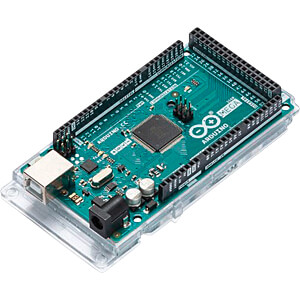
\includegraphics[width=0.5\linewidth]{Bilder/ARDUINO_MEGA.jpg}
	\caption{Arduino Mega (Quelle: \url{https://cdn-reichelt.de/bilder/web/artikel_ws/A300/ARDUINO_MEGA_01_NEU.jpg})}
	\label{fig:arduino_mega}
\end{figure}
\paragraph{Variante B}
Variante B hat als Grundkonzept ein 7-Zoll-Display, welches nicht berührungsempfindlich ist und auch nicht wasserfest, und deswegen wie in Variante A in eine witterungsfeste Box gelegt und durch Buttons gesteuert wird. Neben den unterschiedlichen Bildschirmgrößen unterscheidet auch der verwendete Mikrocontroller die beiden Kombinationen, denn hier wird ein Raspberry PI als Zentralrechner etabliert. Eine Abbildung davon ist in Abbildung \ref{fig:raspi3} zu sehen.\\
Der Gesamtpreis der Hardware liegt bei ungefähr 93.00€ und ist somit auch noch eine der günstigeren Versionen. Für diese Variante sprechen aber noch andere Faktoren. Einerseits die erhöhte Benutzerfreundlichkeit im Vergleich zur Variante A, denn auch wenn wieder Buttons für die Navigation verwendet werden, erleichtert das größere Display die Übersicht. Andererseits die Witterungsfestigkeit aufgrund des Gehäuses, welches bei Schäden leicht und günstig zu ersetzen ist. Auch Dokumentationen sind ausreichend für Hardware und Software vorhanden. Die Probleme hierbei beziehen sich jedoch auf die Verfügbarkeit des Raspberry PIs, da diese in letzter Zeit entweder wenig verfügbar oder teuer sind. Der Display-Preis ist zwar auch nicht niedrig, kann aber durch Mengenrabatte reduziert werden.
\begin{figure}[ht]
	\centering
	\includegraphics[width=0.6\linewidth]{Bilder/RASPBERRY_PI3.png}
	\caption{Raspberry PI 3 (Quelle: \url{https://cdn-reichelt.de/bilder/web/xxl_ws/A300/RASPBERRY_PI_3_02_20210420.png})}
	\label{fig:raspi3}
\end{figure}
\paragraph{Variante C}
Die dritte Variante ist die mit Abstand teuerste, denn hier liegt der Preis bei etwa 117,00€. Der Grund dafür ist, dass die Konzeption aus einem \gls{kapazitiv}n 7-Zoll-Display besteht. Dieses wird unter Abbildung \ref{fig:kapazitives_display} abgebildet. Neben der eigentlich nicht gegebenen Witterungsfestigkeit des Displays per se, wird es jedoch so verbaut, dass diese Eigenschaft trotzdem gegeben ist. Dennoch kann sich möglicherweise die Handhabung der Touchfunktion mit der Zeit aufgrund fehlender Wasserfestigkeit verschlechtern. Da auch hier wieder der Raspberry PI die Grundlage des Systems spielt, ist auch wieder die Verfügbarkeit dessen unpassend. Positive Aspekte sind allgemein die Touchfunktion, da diese weit verbreitet ist und die Bedienung für den Nutzer einfach hält. Ebenso gibt es ausreichend Dokumentationen für Hardware und Software, trotzdem kann die Implementation der Touch-Funktion Probleme bereiten.
\begin{figure}[ht]
	\centering
	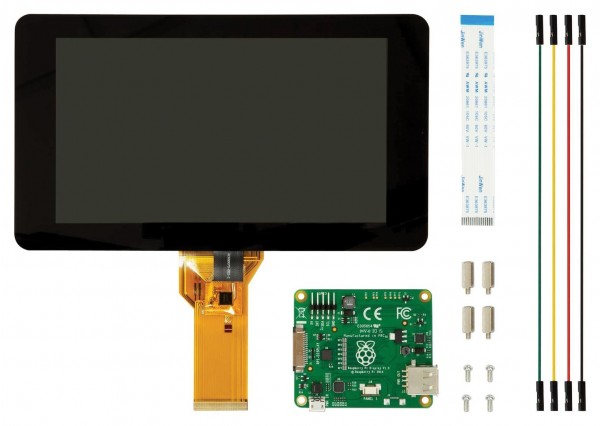
\includegraphics[width=0.6\linewidth]{Bilder/kapazitives_display.jpg}
	\caption{\gls{kapazitiv}s Display (Quelle: \url{https://www.berrybase.at/media/image/49/8e/36/ID_53172_orig_600x600.jpg})}
	\label{fig:kapazitives_display}
\end{figure}
\newpage
\paragraph{Variante D}
Die vierte und letzte Variante charakterisiert sich durch eine weitere Nutzung eines \gls{kapazitiv}n oder diesmal auch \gls{resistiv}n 7-Zoll-Displays, welches nicht wasserdicht ist. Der Zugriff zum Display erfolgt durch eine transparente Klappe am Gehäuse. Eine Abbildung dieses Gehäuses befindet sich unter Abbildung \ref{fig:gehäuse_mit_klappe}. Auch hier wird der Raspberry PI als Mikrocontroller verwendet, welches auf zuvor genannte Probleme bezüglich der Verfügbarkeit zurückführt. Das Display zu erhalten führt zu keinen Schwierigkeiten und man erhält auch wieder einen Mengenrabatt. Nichtsdestotrotz liegt der Gesamtpreis bei ungefähr 108,00€ und ist somit eine der teureren Zusammenstellungen. Dafür stellen Witterungsprobleme keine Erschwernisse dar, solange nicht vergessen wird, die Klappe am Gehäuse immer ordnungsgemäß zu schließen. Die Situation mit den Dokumentationen ist äquivalent zu Variante B und C und somit auch kein Problem. Zurückkehrend auf die unterschiedlichen Displays: Die \gls{kapazitiv} Version hat eine allgemein besser funktionierende Touch-Funktion, die aber durch nasse Hände genommen wird und somit die Nutzung bei beispielsweise Regen erschwert wird. Die \gls{resistiv} Version ermöglicht dafür eine besseren Reaktionsfähigkeit bei nassen Händen oder sogar beim Tragen von Handschuhen.
\begin{figure}[ht]
	\centering
	\includegraphics[width=0.6\linewidth]{Bilder/gehäuse_klappe.png}
	\caption{Gehäuse mit Klappe (Quelle: \url{https://asset.conrad.com/media10/isa/160267/c1/-/de/706888_BB_00_FB/image.jpg?x=1000&y=1000&format=jpg&ex=1000&ey=1000&align=center})}
	\label{fig:gehäuse_mit_klappe}
\end{figure}
\newpage
\paragraph{Bewertungsmatrix}

Um eine umfassende Übersicht über die potenziell verfügbaren Varianten sowie ihre spezifischen Merkmale sicherzustellen, wurde eine detaillierte Bewertungsmatrix in Excel erstellt. Diese Matrix befindet sich auf der nächsten Seite unter Abbildung \ref{fig:matrix}.
\begin{landscape}
	\begin{figure}[H]
		\centering
		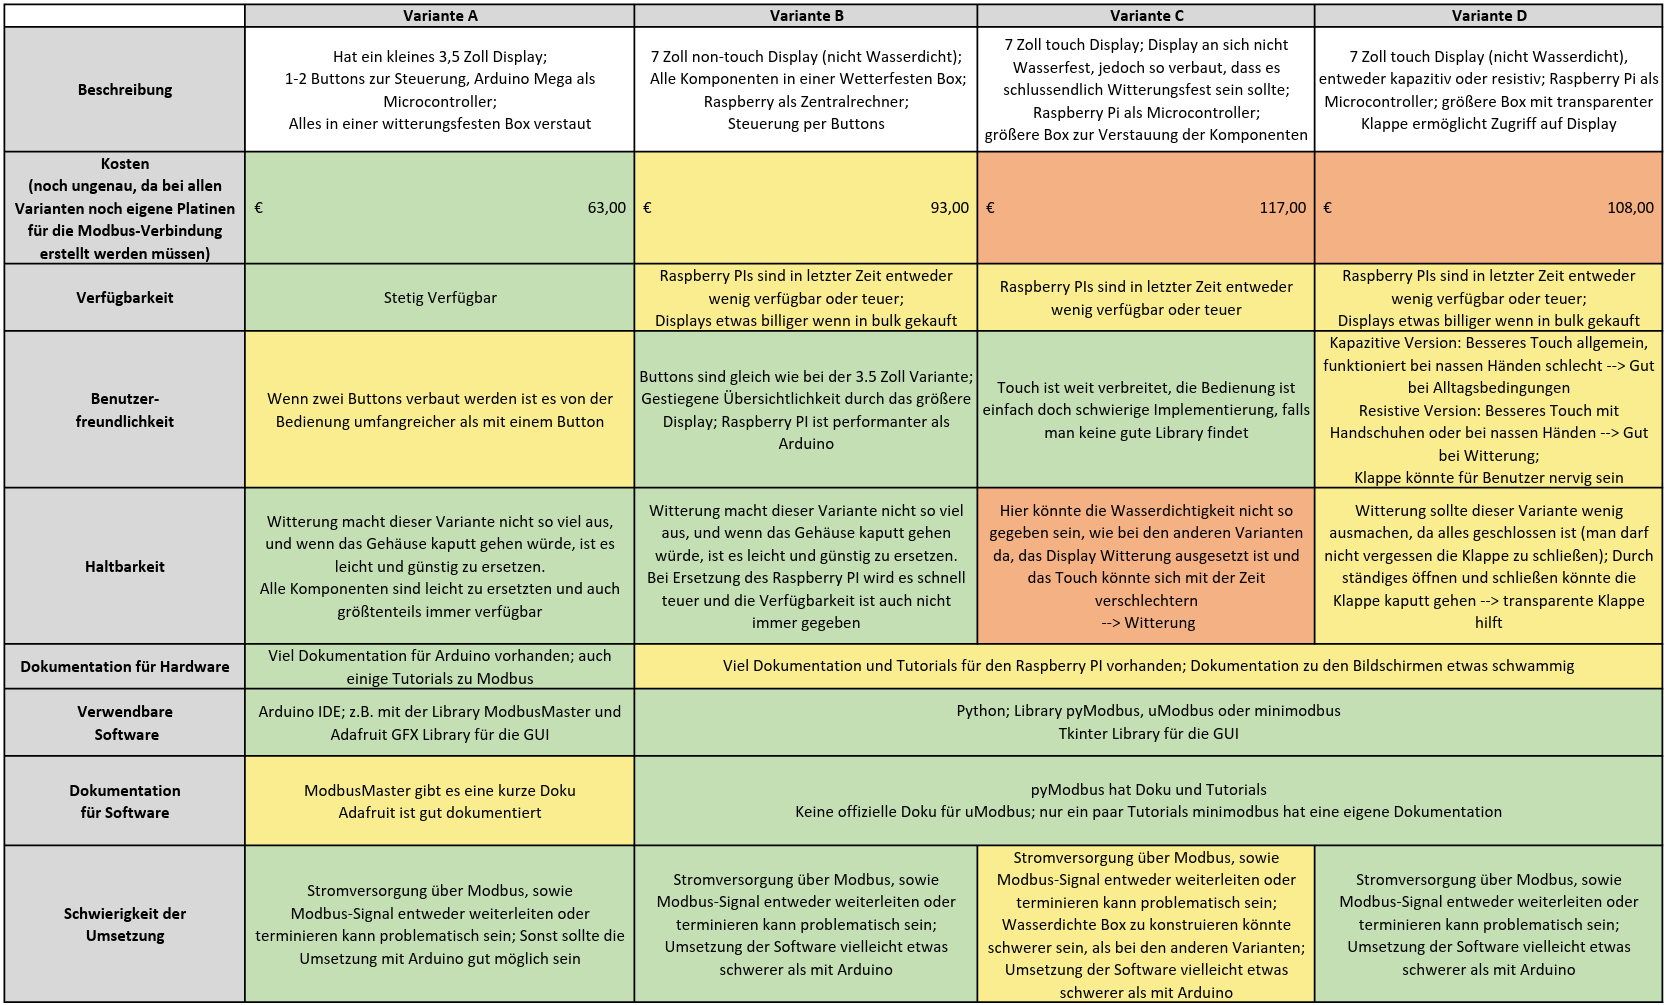
\includegraphics[width=1\linewidth]{Bilder/bewertungsmatrix}
		\caption{Bewertungsmatrix der Hardwarekomponente}
		\label{fig:matrix}
	\end{figure}
\end{landscape}

\setAuthor{\fenkart}
\newpage
\subsection{Selektierung} \label{selektierung}
Die nach Recherche erstellten Varianten im Kapitel \ref{evaluierung}, mussten innerhalb eines Meetings dem Projektbetreuer und einer weiteren Person als Beisitz vorgestellt werden, damit die Varianten auseinandergenommen werden können und auf den Grund gegangen werden kann, welche für die Umsetzung tatsächlich sinnvoll ist und auch auf wirtschaftlicher Ebene vernünftig wäre. Im Folgenden befindet sich eine kurze Beschreibung der jeweiligen Varianten in Kombination mit den im Meeting angemerkten Punkten.

\begin{itemize}
	\item \underline{Variante A:} Hier wäre ein etwas kleineres Display in Verwendung, genauer gesagt ein 3.5-Zoll-Display, mit einem Chipsatz, der anders als bei den anderen Varianten ist, nämlich der Arduino Mega. Für diese Umsetzung müsste eine Platine zwischen Display und Board erstellt werden für die Pins, demnach ist es nicht besonders effizient erweiterbar wie beispielsweise bei dem Raspberry Pi. Bei dieser Version würde alles in ein IP66 geschütztes Gehäuse verbaut werden und mit Buttons gesteuert. Laut Simon Köldorfer sei diese Methode sinnvoller und einfacher als bei der Nutzung eines Touchscreens, da dieser zu viele Funktionen für eine schlichte Anzeige habe und auch nicht sehr geeignet für Witterungen sei. \\
	Da bei dem Arduino nicht sehr viele Libraries für die Benutzeroberfläche zur Verfügung stehen, würde es mit der vom Projektteam gewählten Library weniger schön aussehen, daher, dass diese eine günstige Variante ist, mit der nur Texte, Rechtecke, Linien und Kreise erstellt werden können.
	
	\item \underline{Variante B:} Diese Kombination an Hardware-Komponenten ist der Favorit des Projektteams. Hier wird ein größeres Display mit 7-Zoll und einem Raspberry Pi 3 als Chipsatz verwendet. Die Gesamtheit würde wieder in einer IP66-tauglichen Box verstaut werden. Diese Variante wäre zwar teurer als die 1., dafür könnte die Umsetzung schöner realisiert werden. Auch könnte man sich die RS323-Schnittstelle sparen, da man stattdessen einen USB-Port zur Verfügung hat.
	\item \underline{Variante C:} Variante C ist gleich zu Variante A, nur dass ein Touchdisplay implementiert werden würde, wodurch auch Einsparungen am Gehäuse erfolgen. Diese Einsparung könnte jedoch zu Problemen mit Witterungen wie zu starker Sonneneinstrahlung, Regen, usw. führen. Natürlich gibt es andere, widerstandsfähigere Industriedisplays, diese sind aber auch deutlich teurer und bereits ohne das handelt es sich hier um die teuerste Variante, die zusätzlich nicht wasserfest ist.
	\item \underline{Variante D:} Hier handelt es sich um dasselbe Konzept wie in Variante C, nur dass eine Klappe implementiert ist. Diese müsste immer geöffnet werden, wenn durch die Werte gescrollt werden will, was nicht sehr praktisch ist, da diese kaputtgehen könnte bei zu öfter Verwendung. Auch ist hier die Witterung wieder ein Thema, da das Display bei Regen beispielsweise durch die nicht vorhandene Wasserfestigkeit einen Schaden erhalten könnte.
\end{itemize}

\paragraph{Endgültige Entscheidung}
Durch die überflüssig komplizierte Handhabung des Displays, die unter Verwendung eines Touchdisplays entstehen würde, die zu große Fehleranfälligkeit und die zu hohen anfallenden Kosten, wurden Variante C und D nicht in Erwägung gezogen. \\
Bei Variante A wurde die einfache Darstellung der Werte bemängelt, da es möglicherweise nicht ästhetisch ansprechend wäre. Bezüglich der herzustellenden Platine wurde dazu jedoch angemerkt, dass diese von dem derzeit in der Firma arbeitenden Ferialpraktikanten aus der HTL Rankweil erstellt werden könnte. \\
Zu Variante B wurde gesagt, dass hier die Umsetzung auch mit einem Raspberry Pi Zero funktionieren würde, was weitere Einsparungen bedeuten würde und da der Raspberry Pi auch noch erweiterbar ist und die Version B ein größeres Display hat, wurde sich für diese Variation entschieden.


\section{Software-Selektion}
\setAuthor{\schneider}
Für die Ausarbeitung der Diplomarbeit stehen eine Vielzahl von Programmiersprachen zur Verfügung. Geachtet wurde bei der Auswahl auf die Einfachheit bzw. Vertrautheit der einzelnen Teammitglieder mit der Sprache, deren Funktionalität, das Bibliotheken-Angebot und die vorhandene Dokumentation. In dieser Diplomarbeit wird die Programmiersprache Python verwendet. 

\subsection{Python}
Python ist eine vielseitig einsetzbare Programmiersprache. Eine erste Version wurde 1991 von Guido van Rossum als Hobbyprojekt entwickelt und später als sie erste Erfolge verzeichneten, wurde das Team erweitert. Seither konnte sich Python besonders durch seine einfache Syntax und die vielen vorhandenen Bibliotheken immer stärker etablieren. Im Gegensatz zu Sprachen wie C, C\#, etc. verwendet Python keinen Compiler, um das Coding vor der Ausführung des Programms in Maschinencode umzuwandeln, sondern einen Interpreter, der beim Start des Programms jede Zeile nacheinander überprüft und ausführt. Diese Praktik wurde erstmals mit der Programmiersprache Lisp eingeführt und wird unter anderen von Java, Ruby oder PHP benutzt. 
\cite{Python_Software_Foundation:o.J., Pramanick_gfg:2019, Ryte:2021}

Die folgenden Vor- und Nachteile beziehen sich auf \textcite{Ceaseo:2020}.
\paragraph{Vorteile}
\begin{itemize}
	\item Nicht nur die Syntax ist übersichtlich, sondern auch die Bibliotheken-Verwaltung ist einfach. Mit dem pip-Paketmanager können mit einem „pip install“ alle vorhandenen Bibliotheken installiert werden.
	\item Python kann in den unterschiedlichsten Anwendungen zum Einsatz kommen. Es können damit unteranderem Web-, Mobile- und Backendanwendungen erstellt werden. Außerdem eignet sie sich auch als Skriptsprache für Probleme, bei denen es keiner komplexen Software bedarf. Es können objektorientierte Strukturen genauso wie funktionale verwendet werden. 
\end{itemize}

\paragraph{Nachteile}
\begin{itemize}{}{}
	\item Da die Sprache Zeile für Zeile interpretiert wird, dauert die Ausführung länger als bei kompilierten Sprachen.
	\item Zur Initialisierung einer Variable muss kein Datentyp angegeben werden. Dadurch hat der Programmierer weniger Schreibaufwand, allerdings können in erhöhtem Maße Laufzeitfehler auftreten und auch die Übersichtlichkeit ist betroffen.	
\end{itemize}

\paragraph{Gründe}
Ein ausschlaggebender Grund für die Verwendung von Python ist, dass alle Teammitglieder damit schon Erfahrungen gemacht haben. Beim Einsatz anderer Sprachen wäre die Einarbeitungszeit einzelner Teammitglieder zu berücksichtigen. Außerdem liegt es nahe, da es für den Raspberry PI eine Standardsprache ist. Die oben beschriebenen Nachteile der Sprache sind für ein Proof-of-Concept vernachlässigbar. Außerdem hat die Recherche ergeben, dass viele gut dokumentierte Bibliotheken für Modbus und \aclp{gui} vorhanden sind.

\paragraph{Verwendete Python-Bibliotheken}
Für das Auslesen der \acfp{rlt} Werte über das Modbus Protokoll wird minimalmodbus verwendet. Um die erhaltenen Werte auch grafisch anzuzeigen, wird customtkinter verwendet. Es folgen die Beschreibungen dieser beiden Bibliotheken.


\setAuthor{\pezze}
Raumlufttechnische Anlagen beinhalten unterschiedlichste Komponenten, beispielsweise Ventilatoren, Luftdrucksensoren und Temperatursensoren, mit denen die Funktion überwacht und gesteuert wird. Weil die \acsp{rltanlage} der Firma Bösch auf Kundenanforderungen angepasst werden, ist die Anordnung und Menge der verbauten Komponenten in den meisten Fällen unterschiedlich. Daher ist es wichtig, dass die \acs{rltanzeige} parametrierbar ausgeführt werden kann. Um dies zu erzielen, wurde vom Projektauftraggeber die Idee einer Konfigurationsdatei vorgeschlagen. Mit dieser kann von einer  Servicetechnikerin \bzw einem Servicetechniker bei der Installation der \acs{rltanlage} die Konfiguration an die \acs{rltanzeige} übergeben werden. So können für die jeweilige \acs{rltanlage} immer die richtigen Parameter angezeigt werden.

Wegen der Tatsache, dass diese Konfigurationsdateien von Servicetechnikerinnen und Servicetechnikern erstellt werden müssen, ist es wichtig, dass das gewählte Datenformat für Laien einfach zu verstehen ist. Daher lag die Entscheidung für das richtige Datenformat zwischen \acs{csv} und \acs{json}. Andere Formate  wie \acf{xml} wurden nicht in Erwägung gezogen, weil das Projektteam mit \acs{json} und \acs{csv} schon vertraut war. Darüber hinaus ist \acs{xml} im Vergleich zu \acs{json} für Laien schwerer zu lesen und schreiben, was es für die Anwendung ungeeignet macht. 

\subsection{Was ist CSV?}\label{csv_kapitel}
\acf{csv} ist ein systemunabhängiges Format für Klartextdateien mit der Dateiendung \enquote{.csv}. \acs{csv} Dateien dienen zum Speichern und Übertragen von strukturierten Daten, hauptsächlich Tabellen oder Listen, wobei durch die Verkettung von mehreren \acs{csv} Dateien oder mithilfe von zusätzlichen Regeln auch verschachtelte Objekte gespeichert werden können. Die hauptsächlichen Anwendungsbereiche von \acs{csv} Dateien sind zum Importieren und Exportieren von Daten aus Datenbanken oder die Migration von Tabellendaten zwischen Programmen. \cite[vgl.][]{FuchsMediaSolutions:o.J.}

Die erste Verwendung des Datenformates geht auf 1972 zurück, wo es vom IBM FORTRAN IV (H Extended) Compiler unterstützt wurde. \cite[vgl.][]{IBM:1972} Trotz der langen Existenz gibt es gegenwärtig für \acs{csv} keine formelle Spezifikation. Mit dem \acs{rfc} 4180 \cite[vgl.][]{Shafranovich:2005} aus dem Jahre 2005 existiert ein erster Versuch einer inoffiziellen Definition, welche mittlerweile weit verbreitet ist. Durch dieses Dokument wird das \acf{mime} \enquote{text/csv} für das \acs{csv} Format registriert. Es folgen die wesentlichen Merkmale aus der Definition des \acs{rfc} 4180:

\begin{enumerate}{}
	
	\item Jedem Datensatz steht eine Zeile zu, die mit einem Zeilenumbruch (\ac{crlf}) beendet wird. Ein Zeilenumbruch am Ende des letzten Datensatzes ist optional. \zB 
	\begin{lstlisting}
	aaa, bbb, ccc CRLF
	xxx, yyy, zzz CRLF
	\end{lstlisting}
	oder
	\begin{lstlisting}
	aaa, bbb, ccc CRLF
	xxx, yyy, zzz
	\end{lstlisting}
	
	\item Am Anfang eines \acs{csv} Dokumentes kann es eine Kopfzeile geben. Diese hat das Format eines normalen Datensatzes und beinhaltet Namen für die Spalten (Felder). Die Anzahl der Spalten sollte für Kopfzeile und Datensätze gleich sein. \zB
	\begin{lstlisting}
	spaltenname_1, spaltenname_2, spaltenname_3 CRLF
	xxx, yyy, zzz CRLF
	\end{lstlisting} %	aaa, bbb, ccc CRLF
	
	\item Sowohl in den Datensätzen als auch in der Kopfzeile kann es eine oder mehrere Spalten geben, die jeweils immer durch einen Beistrich (\acs{engl} comma) separiert werden. Am Ende einer Zeile bedarf es keines Beistrichs. Abstände sind Teil eines Feldes und müssen berücksichtigt werden. (Anmerkung: Auch wenn das eigentliche Format Beistriche für die Feldtrennung vorsieht, werden oft andere Zeichen wie \zB Strichpunkte (Semikolons) verwendet.)
	
	\item Jedes Feld kann in Anführungszeichen eingeschlossen sein und darf dann auch Beistriche, Zeilenumbrüche oder Anführungszeichen beinhaltet. \zB
	\begin{lstlisting}
	"aaa","b CRLF
	bb","ccc" CRLF
	xxx,yyy,zzz
	\end{lstlisting}
	
\end{enumerate}

Da es bei \acs{csv} keine festen Vorgaben beim Datenformat gibt, ist es die Verantwortung der Benutzer sich auf eine Formatierung zu einigen. Das führt oft zu Problemen bei Zeit- und Datumsangaben oder bei der Verwendung von Sonderzeichen. Eine weitere Hürde ist die fehlende explizite Angabe des verwendeten Zeichensatzes, womit \zB Umlaute fehlerhaft dargestellt werden können. \cite[vgl.][]{FuchsMediaSolutions:o.J.}

\subsection{Was ist JSON?}\label{json_kapitel}
\begin{minipage}{0.6\textwidth}
	\acf{json} wurde 2001 auf der \enquote{JSON.org} Website veröffentlicht und ist ein ressourcenschonendes Textformat zum Speichern von strukturierten Daten. Es ist so konzipiert, dass es sowohl für Menschen einfach zu lesen und schreiben als auch für Maschinen einfach zu parsen und generieren ist. Die Dateiendung von \acs{json} Dateien ist \enquote{.json}. \acs{json} stammt von JavaScript, ist aber programmiersprachenunabhängig und folgt vielen Konventionen der C-basierten Sprachen, was es gut für den Datenaustausch macht. \cite[vgl.][]{json_org:o.J., ECMA:2017}
\end{minipage}%
\hfill
\begin{minipage}{0.37\textwidth}
	\centering	
	
\includegraphics[width=0.58\textwidth]{JSON_logo}
	\captionof{figure}{\acs{json} Logo (Quelle:\\
		 \url{https://en.m.wikipedia.org/wiki/File:JSON_vector_logo.svg}) \label{fig:json_logo}}
\end{minipage}
\vspace{1ex}

\acs{json} wird derzeit von zwei Spezifikation definiert, ECMA-404 \cite[vgl.][]{ECMA:2017} und RFC 8259 \cite[vgl.][]{Bray:2017}. Dabei unterscheidet sich nur die Beschreibung des Formats, die \acs{json} Syntax beider Spezifikationen ist ident. Folgend wird sich auf die Beschreibung der offiziellen JSON.org Website \cite[vgl.][]{json_org:o.J.} und somit auf ECMA-404 \cite[vgl.][]{ECMA:2017} bezogen.

Die zwei wichtigsten Strukturen auf denen \acs{json} aufbaut sind Name/Wert (\engl Key/Value) Paare und geordnete Listen von Werten. Dabei unterstützt \acs{json} sehr verschachtelte Strukturen. Um diese darzustellen, werden in der Syntax folgende Zeichen benötigt:
\begin{itemize}
	 \item Beistriche \lstinline|,|
	 \item Doppelpunkte \lstinline|:|
	 \item Eckige Klammern \lstinline|[ ]|
	 \item Geschwungene Klammern \lstinline|{ }|
\end{itemize}


Mithilfe dieser Syntax, kann man in \acs{json} folgende Strukturen umsetzen:
\begin{itemize}
	\item \textbf{Values} (\dt Werte) sind, entweder vom Typ \enquote{object}, \enquote{string}, \enquote{array}, \enquote{number} oder haben den Wert \enquote{false}, \enquote{true}, oder \enquote{null} (siehe Abb.~\ref{fig:json_value}).
	\begin{figure}[H]
		\centering
		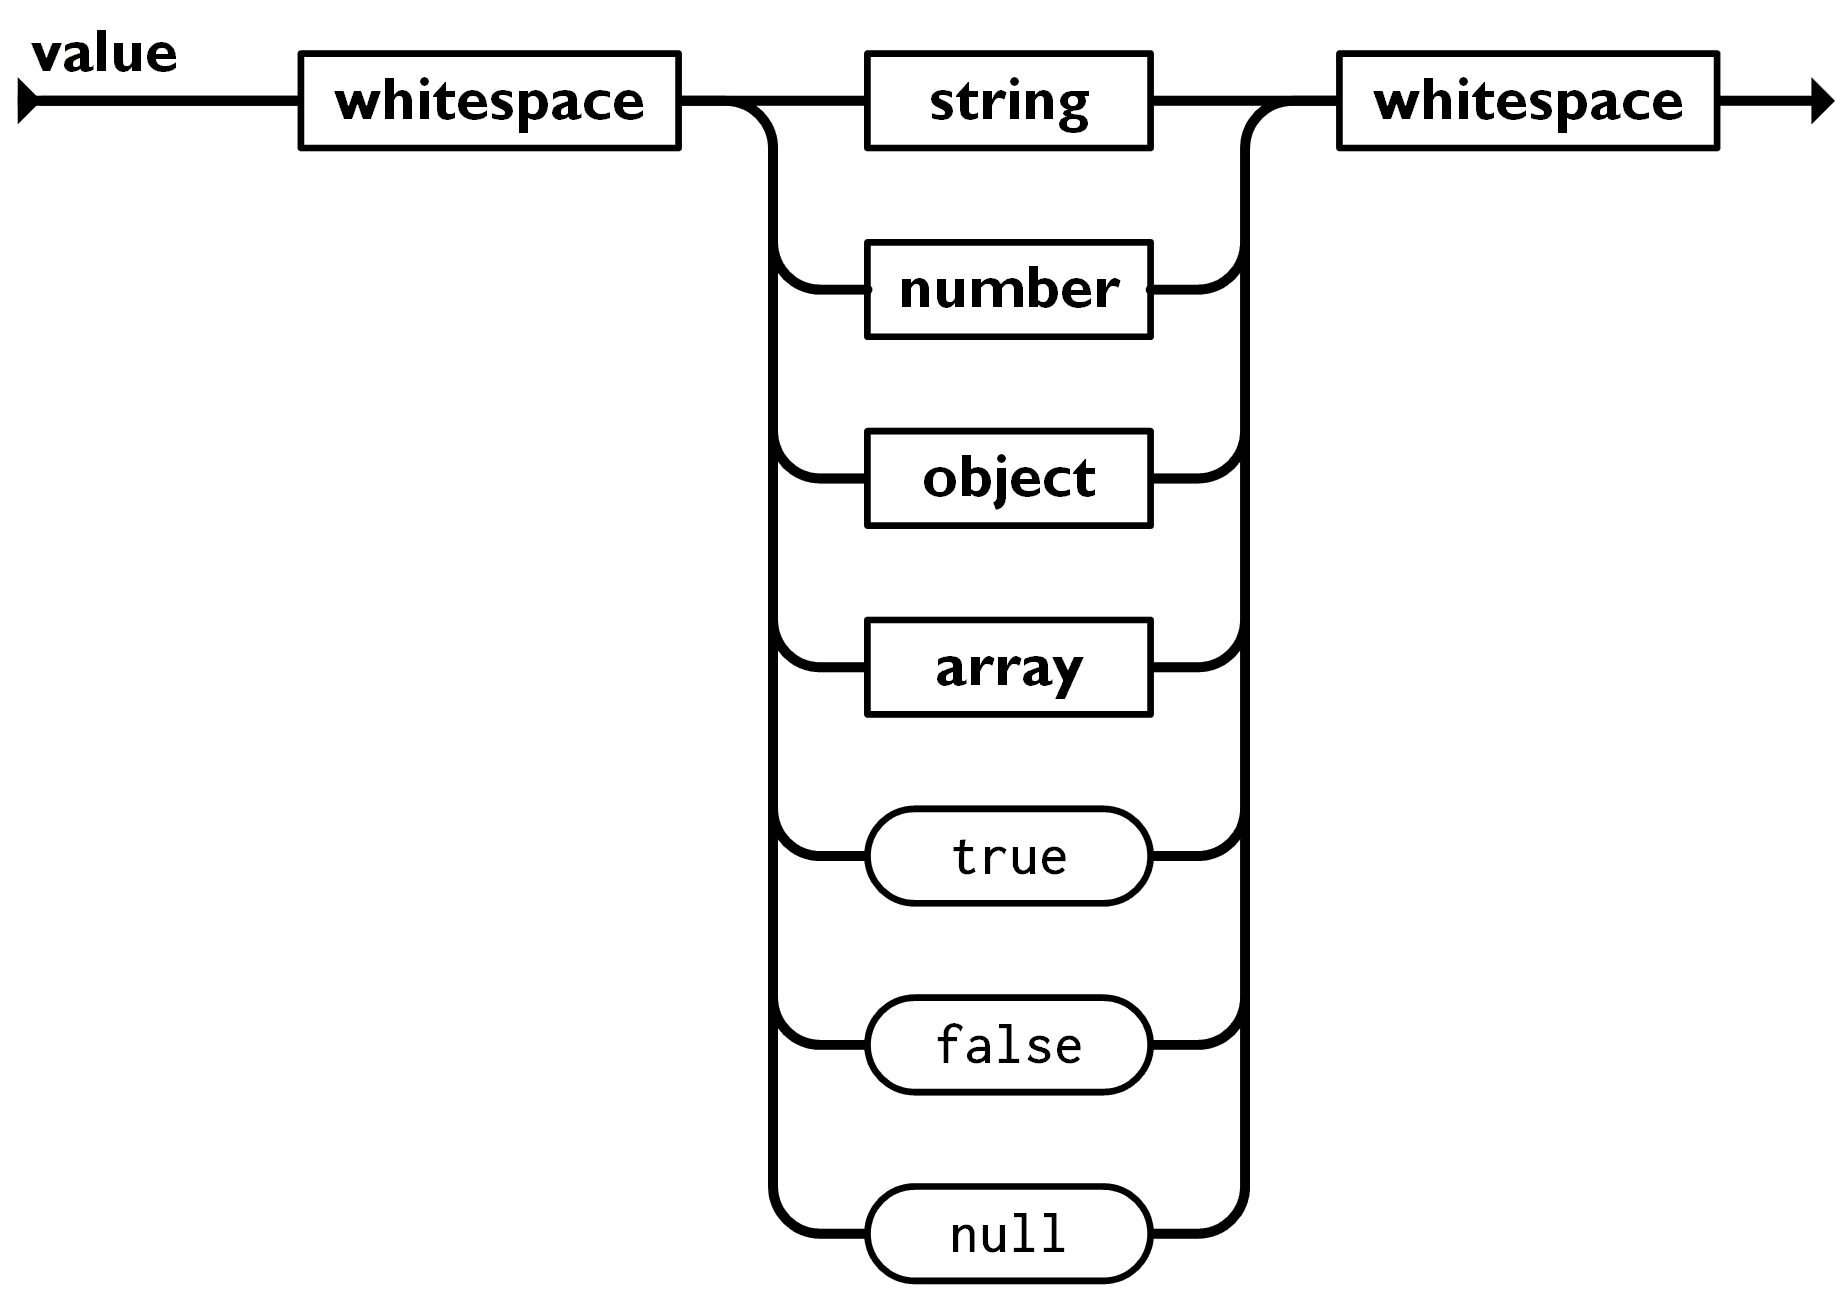
\includegraphics[width=10cm]{JSON_value}
		\caption{\acs{json} Value (Quelle: \url{https://www.json.org/img/value.png})  \label{fig:json_value}}
	\end{figure}
	
	\item \textbf{Objects} (\dt Objekte) sind ungeordnete Listen von beliebig vielen Name/Wert Paaren. Ein Name/Wert Paar besteht immer aus einem Namen, gefolgt von einem Doppelpunkt und dem zugehörigen Wert. Beistriche kommen zum Einsatz um Name/Wert Paare voneinander zu trennen. Ein Objekt wird immer von geschwungenen Klammern umschlossen. Der Aufbau eines \acs{json} Objekts ist in Abb.~\ref{fig:json_object} zu sehen.
	
	\begin{figure}[H]
		\centering
		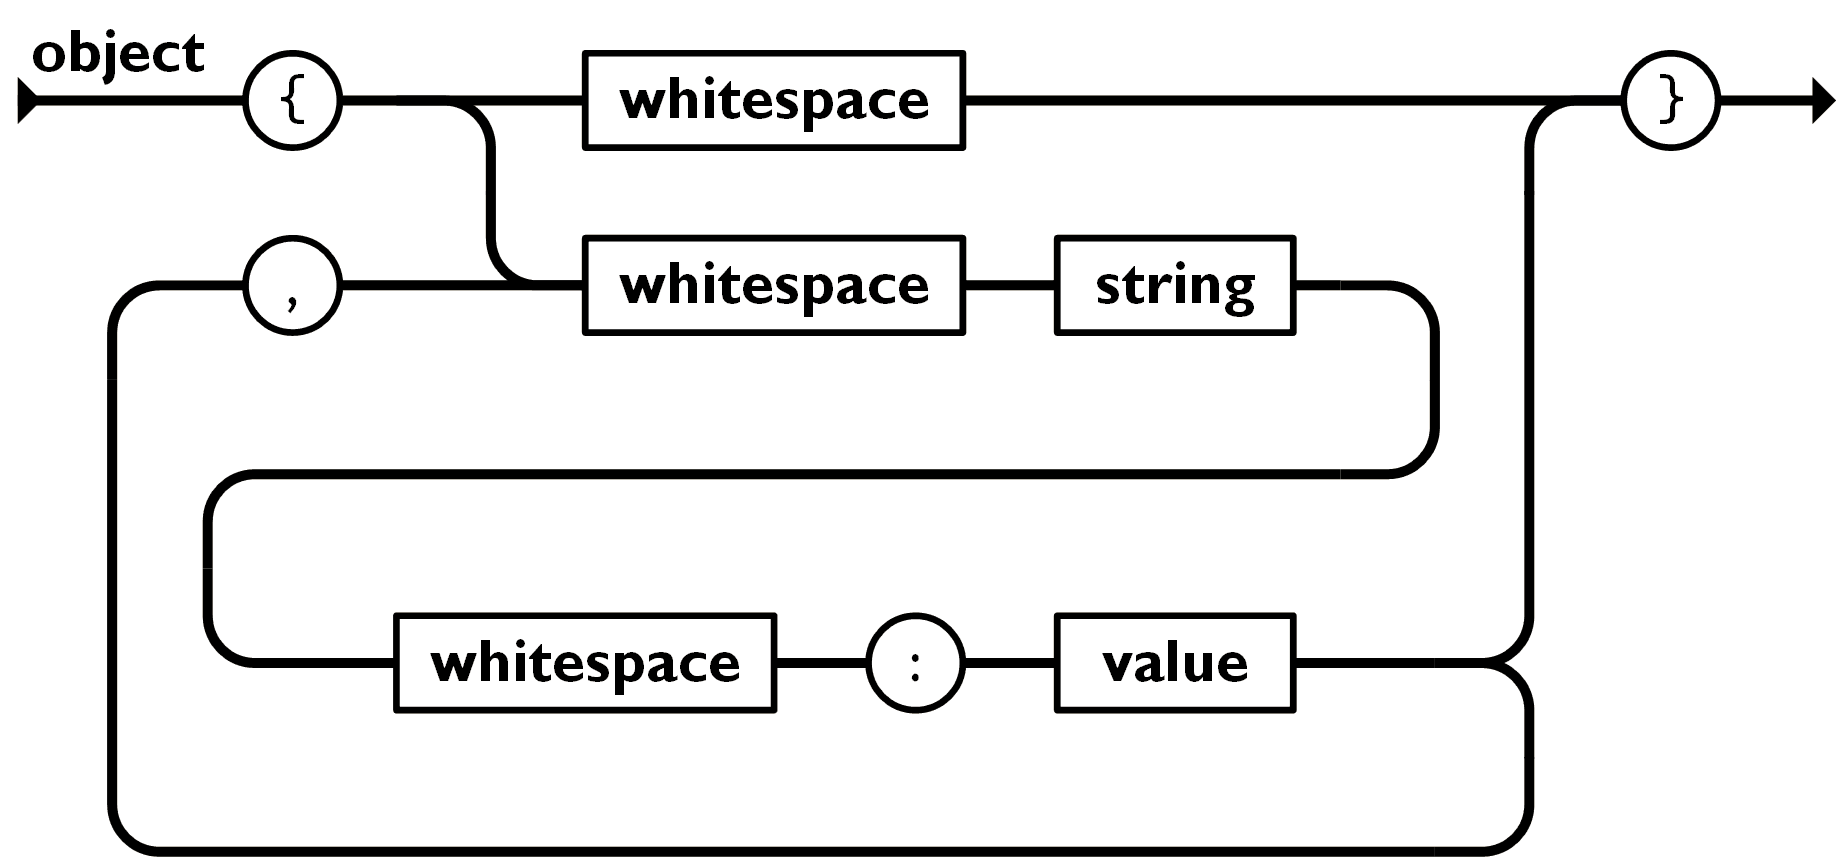
\includegraphics[width=10cm]{JSON_object}
		\caption{\acs{json} Object (Quelle: \url{https://www.json.org/img/object.png})  \label{fig:json_object}}
	\end{figure}
	
	\item \textbf{Arrays} sind geordnete Listen von Werten. Dabei werden Beistriche verwendet, um die Werte voneinander zu trennen. Ein Array wird immer von eckigen Klammern umschlossen. Der Aufbau eines Arrays ist in Abb.~\ref{fig:json_array} zu sehen.
	
	\begin{figure}[H]
		\centering
		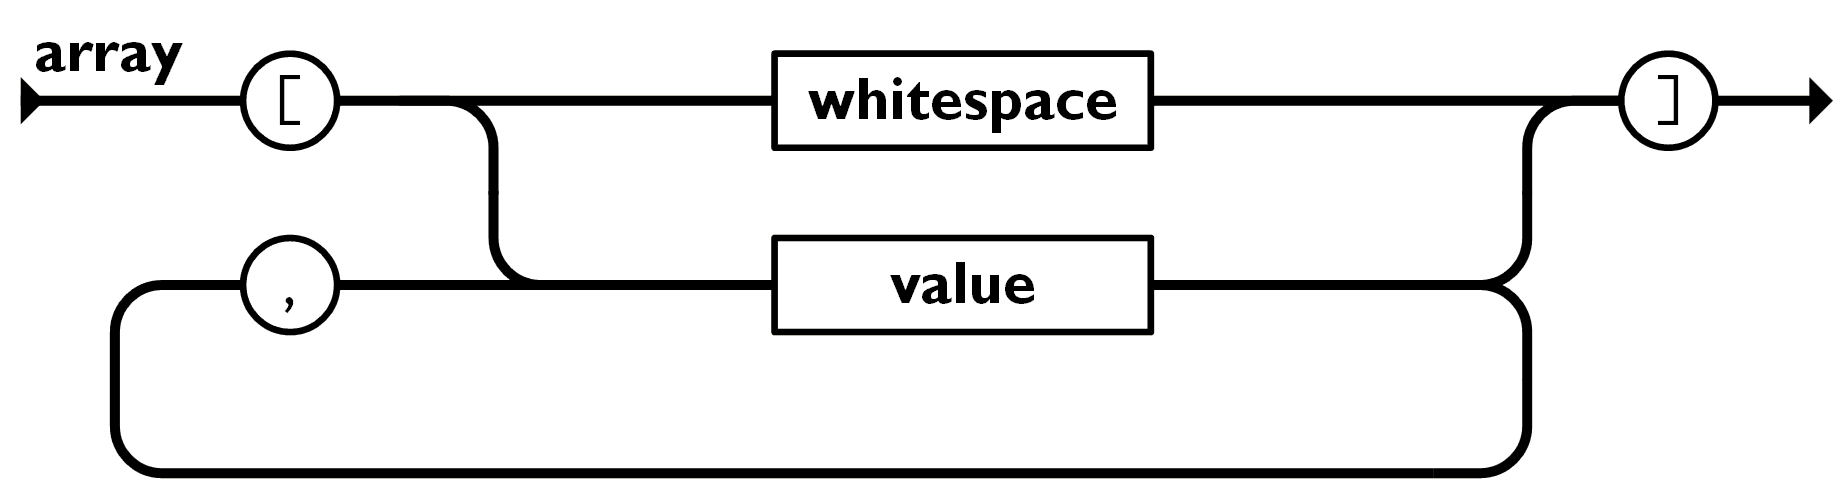
\includegraphics[width=10cm]{JSON_array}
		\caption{\acs{json} Array (Quelle: \url{https://www.json.org/img/array.png})  \label{fig:json_array}}
	\end{figure}
	
	\item \textbf{Strings} sind Zeichenketten. Sie können entweder leer sein, d. h. aus keinen Zeichen bestehen oder mehrere Unicode Zeichen enthalten. Eine Zeichenkette wird immer von Anführungszeichen umschlossen. Sie kann auch besondere Escapesequenzen beinhalten, die besondere Bedeutungen haben. Diese werden mit einem Backslash aufgerufen, wie \zB \enquote{\textbackslash n}, \enquote{\textbackslash t} oder \enquote{\textbackslash r}.
	
	\item \textbf{Numbers} (\dt Zahlen) sind numerische Werte, die aus einer oder mehreren dezimalen Ziffern bestehen. Sie können also keine Werte wie \zB \enquote{Infinity} oder \enquote{NaN} annehmen. Außerdem werden sie nie von Anführungszeichen umschlossen. 
	
\end{itemize}

Beispiele für \acs{json} Dateien sind in Kapitel \ref{json_config_files} zu finden.

\subsection{\acs{json} und \acs{csv} - Vergleich und Selektion} \label{json_vs_csv}
Sowohl \acs{json} als auch \acs{csv} bringen Vorteile mit sich. 
\acs{csv} Dateien können in Microsoft Excel bearbeitet und erstellt werden. Die tabellarische Darstellung und die Bekanntheit von Excel machen es zugänglich für Laien, was der größte Vorteil für \acs{csv} ist. Außerdem wird \acs{csv} von vielen Programmiersprachen unterstützt, was die Umsetzung theoretisch möglich machen würde. 

\acs{json} Dateien sind hingegen \acs{csv} zwar für Laien schwererer zu lesen, bieten aber hinsichtlich meist anderer Aspekte deutlich mehr Möglichkeiten. Anstatt des tabellarischen Aufbaus wird zum Speichern der Daten eine klare hierarchische Struktur verwendet. Die Struktur sorgt für mehr Flexibilität und eine besonders gute Darstellung verschachtelter Daten. Auch unterstützt \acs{json} unterschiedliche Datentypen, während bei \acs{csv} grundsätzlich nur Zeichenketten zum Einsatz kommen.

\acs{json} ist mittlerweile an Kompatibilität kaum zu übertreffen, was dessen Verwendung unbedenklich macht. Das Datenformat wird in unzähligen Bereichen eingesetzt und der Trend scheint immer weiter gegen \acs{json} zu gehen.

Schließlich überwiegen, im benötigten Anwendungsbereich, die vielen Vorteile von \acs{json} die schlechtere Leserlichkeit. Vor allem war die Möglichkeit der Verschachtelung der ausschlaggebende Grund weshalb sich für das \acs{json} Datenformat entschieden wurde. Dazu ist es wahrscheinlich, dass, wegen ihrem logischen Aufbau und  Skalierbarkeit, \acs{json} Dateien für den Anwendungszweck im Endeffekt übersichtlicher als \acs{csv} Dateien sind.

Falls bei Einführung der \acs{rltanzeige} Schwierigkeiten mit der Konfiguration auftreten steht \zB die Option eines Skripts, welches Excel Dateien in das gewünschte \acs{json} Format übersetzt, zur Verfügung.


\chapter{Umsetzung}

\section{Raspberry PI Aufsetzung}
\setAuthor{\pezze}
\label{raspi_setup}
In diesem Kapitel werden kurz die erforderlichen Schritte erläutert, um einen Raspberry PI zur Entwicklung der \ac{rltanzeige} aufzusetzen.
Zur Entwicklung der Diplomarbeit wurden unterschiedliche Versionen des Raspberry PIs genutzt (Raspberry PI 3 Modell B, Raspberry PI Zero). Dabei wird ein Standard Raspberry PI OS (Version 11 \enquote{bullseye}) verwendet, das leicht adaptiert wird.

\subsection{Headless Setup}\label{raspi_headless_setup}
Während der Entwicklung der \ac{rltanzeige} wird mit mehreren Raspberry PIs gearbeitet, die nicht alle gleichzeitig an einem externen Bildschirm angeschlossen werden können. Außerdem verfügt das Raspberry PI Zero Modell aufgrund seiner geringen Größe nur über einen Mini-\ac{hdmi} Anschluss, wofür ein spezielles Kabel \bzw ein spezieller Adapter benötigt wird, und somit nicht einfach ein externer Bildschirm angeschlossen werden kann. Daher wird ein sog. \enquote{Headless Setup} notwendig, bei dem der Raspberry PI ohne angeschlossenen Bildschirm, Tastatur oder Maus gestartet werden kann. Mittels \ac{ssh} oder \ac{vnc} Client kann dann auf den Raspberry PI zugegriffen werden.
\cite[vgl.][]{Piltch:2022} n 

\paragraph{Aktivierung von \textit{SSH}}
\ac{ssh} ist ein Netzwerkprotokoll, das verwendet wird, um sich sicher über das Netzwerk mit einem anderen Gerät zu verbinden und darauf Operationen auszuführen. \ac{ssh} ist am Raspberry PI standardmäßig deaktiviert.  Daher muss \ac{ssh}, durch das Erstellen einer Datei Namens \enquote{ssh.} auf der SD-Karte, aktiviert werden. Nun kann eine kabellose oder kabelgebundene \ac{ssh} Verbindung mit dem Raspberry PI aufgebaut werden.

\paragraph{Kabellose Verbindung über \textit{SSH}}
Für eine kabellose Verbindung über \ac{ssh} muss zuerst auf dem Raspberry PI ein Netzwerkzugang konfiguriert werden. Dazu wird auf der SD-Karte eine Konfigurationsdatei Namens \enquote{wpa\_supplicant.conf} mit folgendem Inhalt angelegt:
\begin{textcode}
country=DE
ctrl_interface=DIR=/var/run/wpa_supplicant GROUP=netdev
update_config=1

network={
    scan_ssid=1
    ssid="[SSID]"
    psk="[Passwort]"
}
\end{textcode}

Nach dem ersten Start lässt sich nun der Raspberry PI mit dem folgenden Befehl über die Kommandozeile verbinden:
\begin{minted}{console}
ssh [Username]@[IP-Adresse]
\end{minted}

\paragraph{Kabelgebundene Verbindung über \textit{SSH}}
Da die normale Version des Raspberry PI Zero keine kabellose Netzwerkverbindung unterstützt, ist es notwendig, eine kabelgebundene Verbindung herzustellen, um \ac{ssh} zu verwenden. Dazu sind folgende Schritte notwendig:

\begin{enumerate}
    \item Am Ende der Datei \enquote{config.txt} auf der SD-Karte folgende Zeile hinzufügen: \begin{textcode}
    dtoverlay=dwc2.
    \end{textcode}
    \item In der Datei \enquote{cmdline.txt} nach \enquote{rootwait} (mit genau einem Leerzeichen dazwischen) folgendes hinzufügen:
    \begin{textcode}
    modules-load=dwc2,g_ether
    \end{textcode}
    \item Den Raspberry PI Zero über USB mit einem Computer verbinden, wobei am Raspberry PI der Daten-USB-Anschluss verwendet werden muss und nicht der Strom-USB-Anschluss.
    \item Apple Bonjour-Druckdienste auf dem Windows Computer herunterladen.
    \item Nun lässt sich nun der Raspberry PI mit dem folgenden Befehl über die Kommandozeile verbinden:
    \begin{minted}{console}
ssh [Username]@[RaspberryPIZero-Name].local
    \end{minted}
\end{enumerate}

\subsection{Installieren der nötigen Python Pakete}
Nach dem Aufsetzen des Raspberry PI OS und \ac{ssh} müssen zuletzt noch die Python Pakete für \gls{gls_tk}, \gls{gls_ctk} und \gls{gls_minimalmodbus} mit den folgenden Befehlen über die Konsole installiert werden:

\begin{minted}{console}
pip install tk
pip install customtkinter
pip install minimalmodbus
\end{minted}


\section{\acf{gui}}\label{gui_design}
\setAuthor{\pezze}
\subsection{Figma Design}\label{figma_design}
\begin{minipage}{0.6\textwidth}
    Zur Erstellung eines Mockups für das Design der \acs{gui} für die \acs{rltanzeige} wurde Figma verwendet. Figma Design ist eine Applikation zum Erstellen von Prototypen im Bereich \ac{uxui}. Dabei kann im Team in Echtzeit zusammen gearbeitet werden. Mit Figma können in das erstellte Design direkt interaktive Funktionen eingebaut werden, um ein realistisches Prototyping zu ermöglichen. Ein weiterer Vorteil von Figma ist der sog. \enquote{Dev Mode}. Mit diesem können Entwickler direkt auf das Design zugreifen und Details finden, die benötigt werden, um das Design in Code umzusetzen. \cite[vgl.][]{figma_design:o.J.}
\end{minipage}%
\hfill
\begin{minipage}{0.37\textwidth}
	\centering	
	
\includegraphics[width=0.50\textwidth]{figma_logo}
	\captionof{figure}{Figma Logo (Quelle: 
		\url{https://en.m.wikipedia.org/wiki/File:Figma-logo.svg}) \label{fig:figma_logo}}
\end{minipage}
\vspace{1ex}

Bei Erstellung des Designs für die \acs{rltanzeige} liegt die Priorität auf Übersichtlichkeit und guter Leserlichkeit. Die Wahl eines 3,5-Zoll Displays hätte (mit ausreichender Übersichtlichkeit) lediglich die simultane Darstellung von maximal zwei Werten erlaubt. Die tatsächliche Wahl eines 7-Zoll Displays zur Anzeige ermöglicht hingegen die zeitgleiche Darstellung mehrerer Werte, wobei fünf bis sechs Werte den idealen Kompromiss zwischen genug Information und Übersichtlichkeit bieten. Um die Übersichtlichkeit weiter zu erhöhen ist die Kategorisierung der Messwerte in sinnvolle und zusammenhängende Seiten wichtig. Alle Informationen zu wichtigen Temperaturen sollen beispielsweise auf einer Seite gruppiert sein, während alle Informationen zu einem bestimmten Ventilator auf einer anderen Seite zu finden sind. Hierbei benötigt jede jeweilige Seite eine Überschrift zur Orientierung. Zusätzlich sollte es eine Indikation geben, die der Nutzerin oder dem Nutzer signalisiert, auf welcher Seite sie oder er sich gerade befindet. Tasten zum Seiten wechseln werden nicht benötigt, da an der \acs{rltanzeige} zwei Taster verbaut sind.

\begin{figure}[H]
    	\begin{subfigure}[t]{0.49\textwidth}
    		\centering
    		\frame{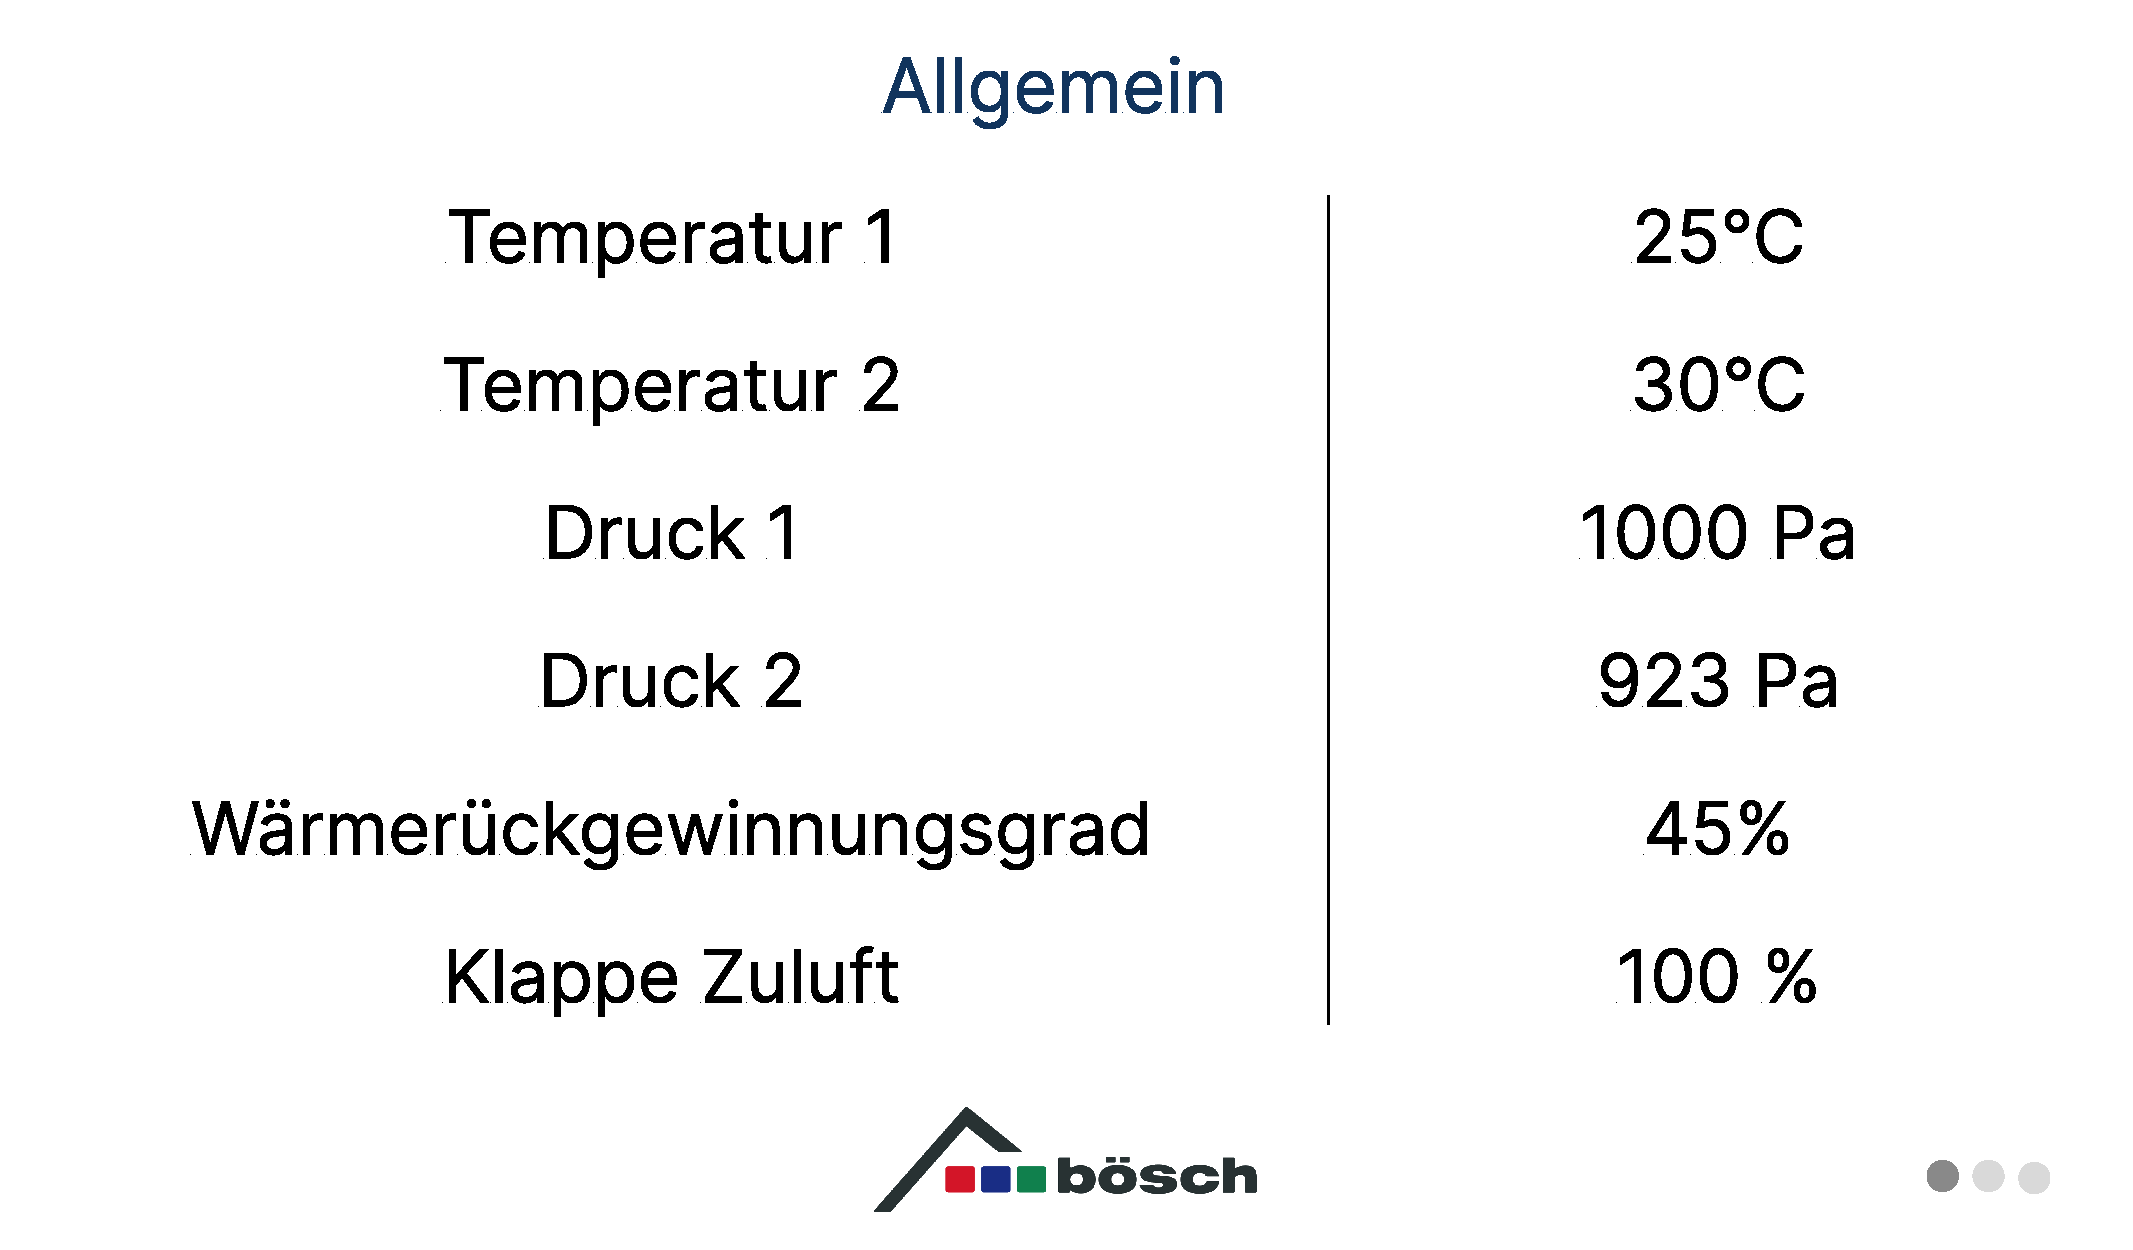
\includegraphics[width=0.99\textwidth, page=1]{design_varianten}}
    		\caption{Design Variante A \label{fig:variante_a}}
    	\end{subfigure}
        \hfill
    	\begin{subfigure}[t]{0.49\textwidth}
    		\centering
    		\frame{\includegraphics[width=0.99\textwidth, page=2]{design_varianten}}
    		\caption{Design Variante B \label{fig:variante_b}}
    	\end{subfigure}
    \begin{subfigure}[t]{\textwidth}
		\centering
		\frame{\includegraphics[width=0.70\textwidth, page=3]{design_varianten}}
		\caption{Design Variante C \label{fig:variante_c}}
	\end{subfigure}
	\caption{\acs{gui} Design Varianten \label{fig:design_varianten}}
\end{figure}

Mit den zuletzt genannten Kriterien wurden drei Designvarianten entworfen (siehe Abb. \ref{fig:design_varianten}). Zur Umsetzung gelangte schlussendlich Variante C (siehe Abb. \ref{fig:variante_c}). Diese bietet mit dem Kontrast im Hintergrund jedes einzelnen Messwerts und der listenartigen Aufzählung die besten Eigenschaften, um Messwerte auf einem Display mit begrenzter Auflösung und Helligkeit in Umgebungen mit suboptimalen Bedingungen ablesen zu können. 


\subsection{Umsetzung der GUI im Code}\label{tkintercode}
\paragraph{Klassenstruktur}
Im Vordergrund basiert die Klassenstruktur grundsätzlich auf \gls{gls_ctk} Komponenten (siehe Abb.~\ref{fig:klassenstruktur_frontend}). Dabei gibt es die Klassen \lstinline{App}, \lstinline{PageFrame}, \lstinline{TitleFrame} und \lstinline{MeasurementFrame}. Im Programm wird eine \lstinline{App} Instanz ausgeführt, welche das Hauptfenster ist. Diese Instanz kann beliebig viele \lstinline{PageFrames} enthalten, die wiederum jeweils ein \lstinline{TitleFrame} und eine Liste von \lstinline{MeasurementFrames} beinhalten. Die \lstinline{PageFrames} stellen die einzelnen Seiten dar, welche per Knopfdruck an der \acs{rltanzeige} durchgeblättert werden können. In einem \lstinline{TitleFrame} wird immer der Titel der jeweiligen Seite gespeichert \bzw angezeigt. In den \lstinline{MeasurementFrame} Instanzen werden hingegen die tatsächlichen Messwerte (Bezeichnung + Wert + Maßeinheit) dargestellt.

\begin{figure}[H]
	\centering
	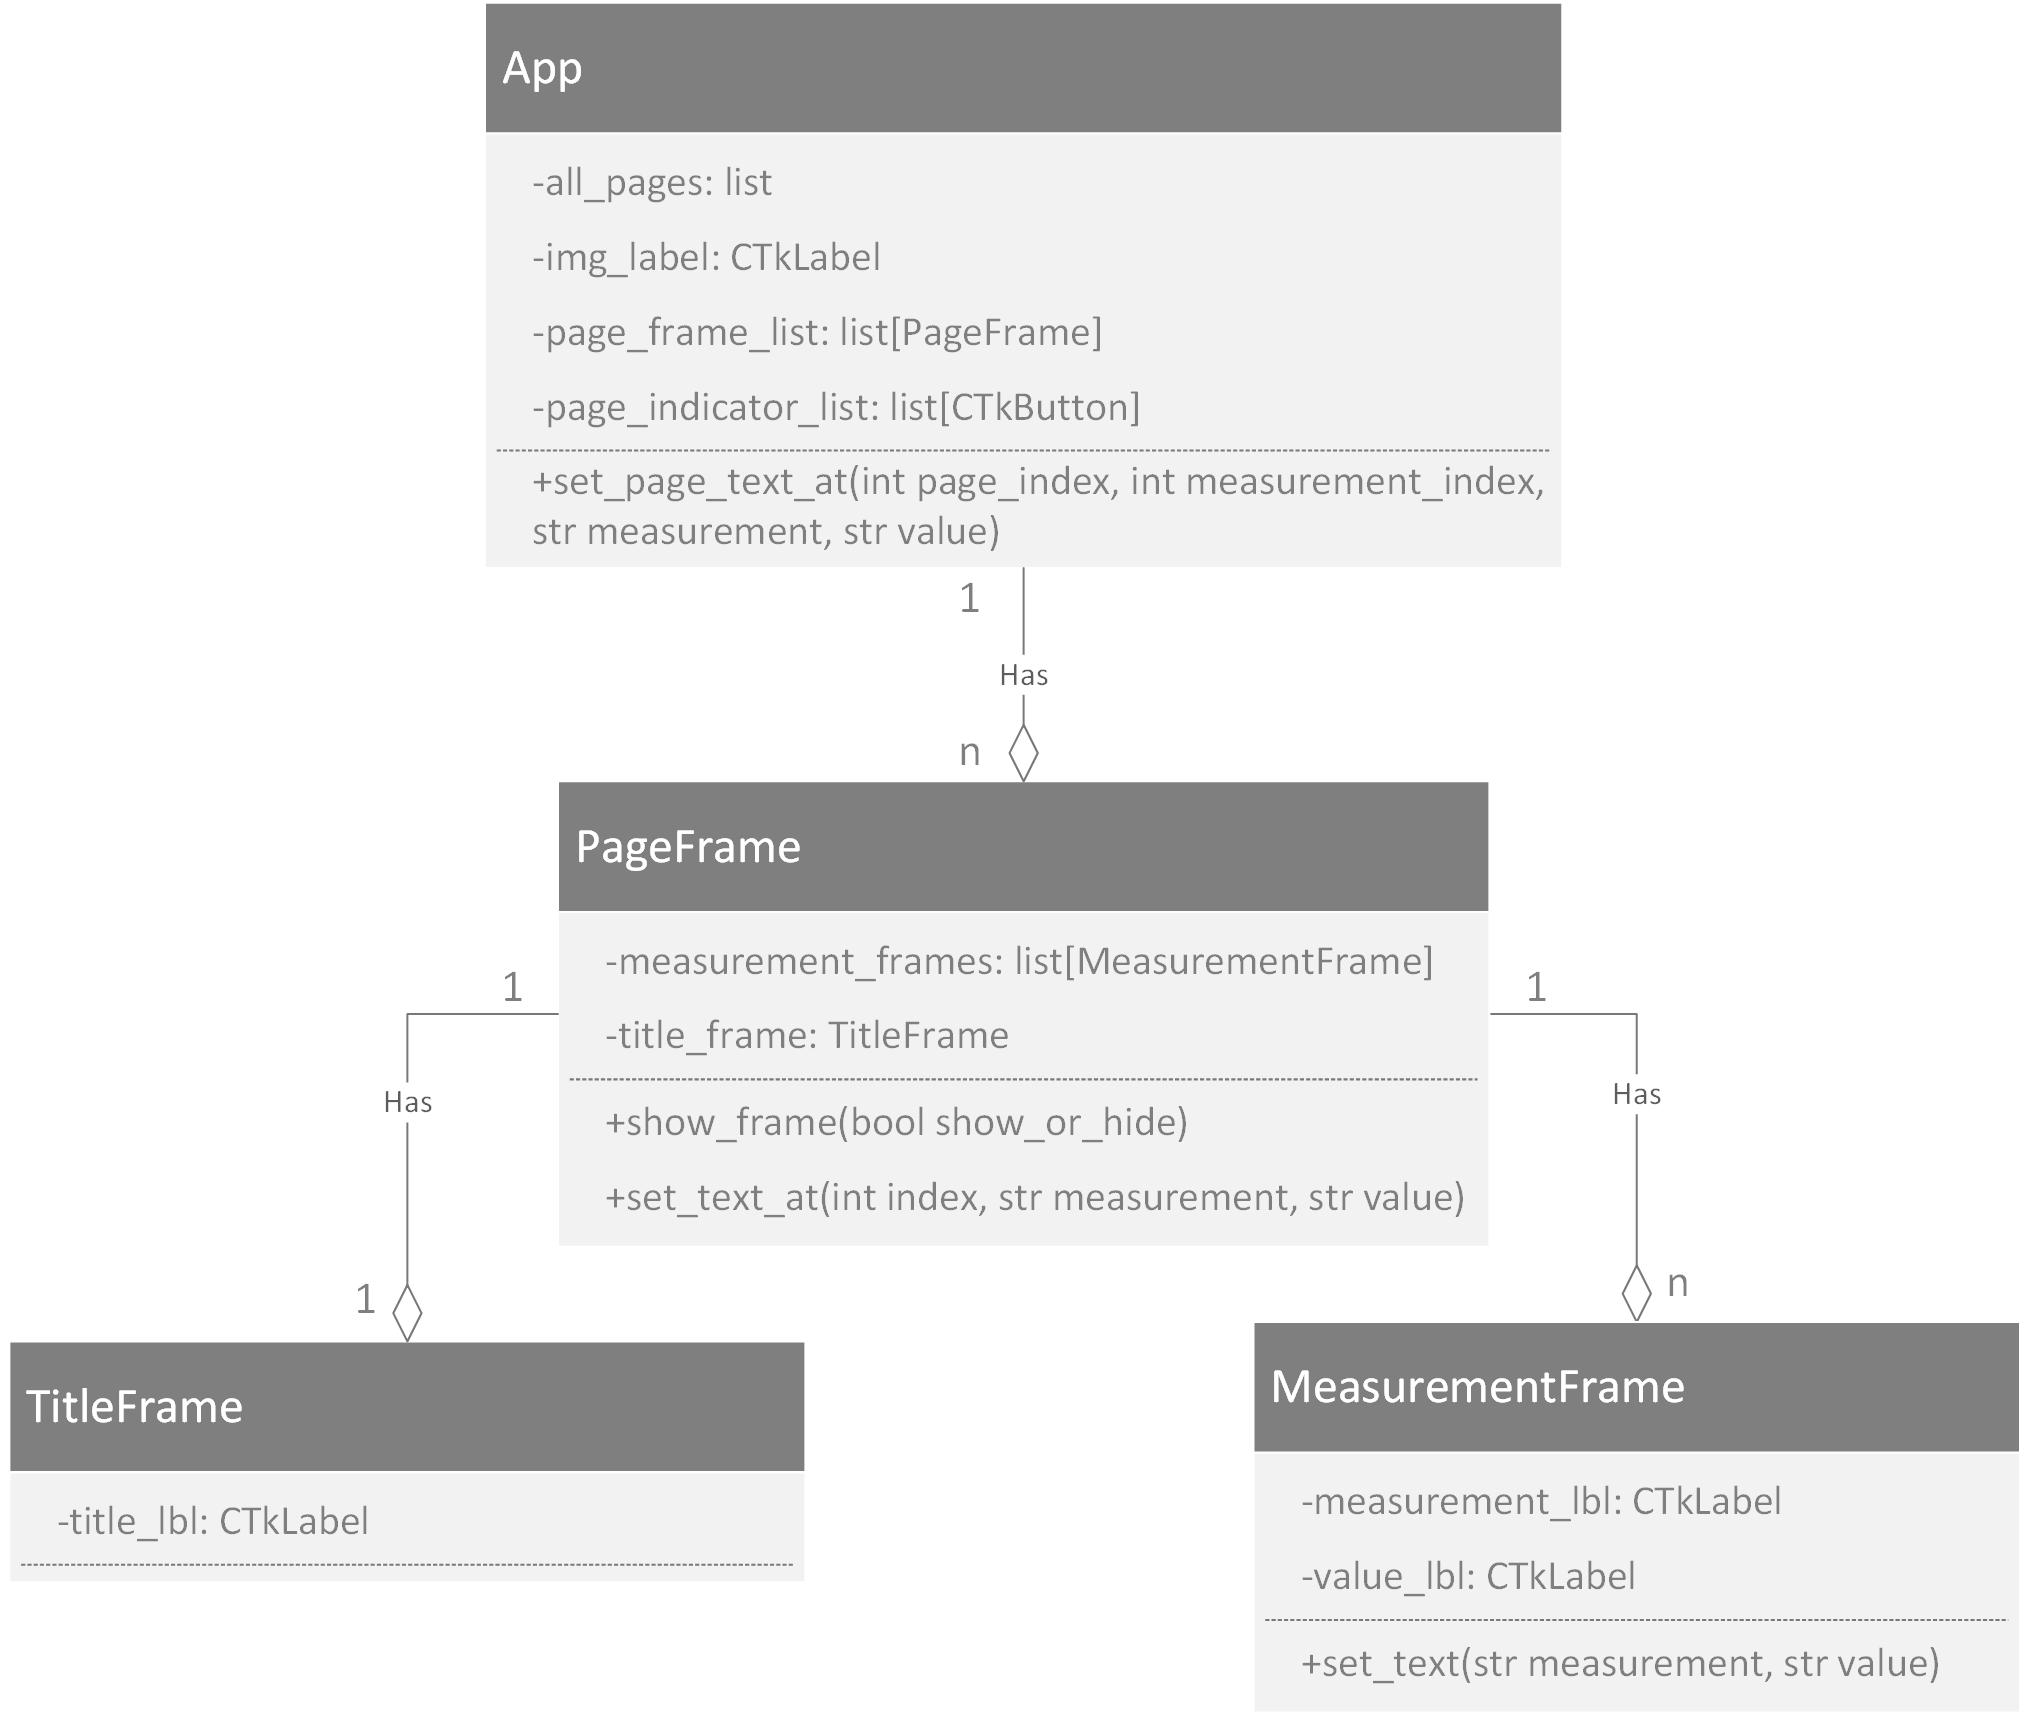
\includegraphics[width=0.95\textwidth]{uml_frontent_class_diagram}
	\caption{UML Diagramm Frontend \label{fig:klassenstruktur_frontend}}
\end{figure}

\paragraph{CustomTkinter Code}

Eine nähere Beschreibung und die Umsetzung der vorher genannten Klassen erfolgt in diesem Kapitel. 
\newline Wie zuletzt beschrieben, basieren alle Klassen im Frontend auf \gls{gls_ctk}. Die Klassen sind dabei alle (bis auf die Klasse \lstinline{App}) vom Typ \lstinline{CTkFrame}. Ein \lstinline{CTkFrame} ist ein Widget, das wie ein Rahmen \bzw Behälter für andere Widgets fungiert. So können diese in weiteren Widgets gruppiert und besser organisiert werden. Als erster Parameter wird für \lstinline{CTkFrames}, wie bei allen \gls{gls_tk} und \gls{gls_ctk} Widgets, der \lstinline{master} \bzw das Elternobjekt angegeben. Darüber hinaus können die Breite (\lstinline{width}), Höhe (\lstinline{height}), Rahmenbreite \bzw -Farbe (\lstinline{border_width} \bzw \lstinline{border_color}) sowie die Hintergrundfarbe (\lstinline{fg_color}) angegeben werden. \cite[vgl.][]{Schimansky:o.J.}

Die Klasse \lstinline{TitleFrame} enthält ein \lstinline{CTkLabel}, welches mit der \lstinline{place()} Methode im Behälter platziert wird. Die Klasse \lstinline{CTkLabel} basiert auf der Klasse \lstinline{tkinter.Label} und dient zur Darstellung eines Textes. Im \lstinline{TitleFrame} Label steht immer der Titel der zugehörigen Seite. Das \lstinline{title_font} Objekt, welches im folgenden Code zu sehen ist, ist eine Instanz der \gls{gls_ctk} Utility Klasse \lstinline{CTkFont}. Es wird verwendet, um die Schriftformatierung von \gls{gls_ctk} Widgets vorzunehmen. Jedes \gls{gls_ctk} Widget bekommt standardmäßig ein \lstinline{CTkFont} Objekt, wobei ein solches Objekt zeitgleich mehreren Widgets angefügt werden kann. Eine Änderung eines \lstinline{CTkFont} Objekts wird an alle Widgets, die es verwenden, weitergeleitet. \cite[vgl.][]{Schimansky:o.J.}

\begin{pythoncode}
class TitleFrame(ctk.CTkFrame):
	def __init__(self, master, title, **kwargs):
		super().__init__(master, width=800, height=60, fg_color=text_color, **kwargs)
		
		title_font = ctk.CTkFont(family="Roboto", size=32)
		
		self.title_lbl = ctk.CTkLabel(master=self, text=title, width=700, height=45, fg_color="transparent", text_color=title_color, anchor=ctk.CENTER, font=title_font)
		self.title_lbl.place(relx=0.5, rely=0.12, anchor=ctk.N)
\end{pythoncode}


Wie in der Klassenstruktur beschrieben, beinhaltet ein jedes \lstinline{PageFrame} neben einem \lstinline{TitleFrame} eine Liste von \lstinline{MeasurementFrames}. Eine Instanz der Klasse \lstinline{MeasurementFrame} enthält immer Informationen zu einem bestimmten Messwert, welche mithilfe von zwei \lstinline{CTkLabel} Widgets dargestellt werden. Dabei wird die Bezeichnung des Messwerts links im \lstinline{measurement_lbl} und der tatsächliche Wert einschließlich Maßeinheit rechts im \lstinline{value_lbl} platziert. Die zwei Labels werden durch einen Strich getrennt, der mit dem \gls{gls_tk} Widget \enquote{Canvas} erstellt wird. Ein Canvas ist ein rechteckiger Bereich \bzw eine Leinwand, auf dem Bilder oder andere komplexe Layouts gezeichnet werden können. Zusätzlich lassen sich auf einem Canvas Widget \zB weitere Widgets, Text oder Bilder platzieren. \cite[vgl.][20]{Shipman:2013} 
\newline Da jeder Messwert kontinuierlich aktualisiert wird, verfügt die \lstinline{MeasurementFrame} Klasse über die Methode \lstinline{set_text()}. In dieser wird mithilfe der \lstinline{configure()} Methode der Text beider Labels aktualisiert. Es folgt ein gekürzter Code zur \lstinline{MeasurementFrame} Klasse.

\begin{pythoncode}
class MeasurementFrame(ctk.CTkFrame):
	def __init__(self, master, measurement, value, **kwargs):
		#[Initialisierung des CTkFrames + Erstellung eines CTkFont Objekts zur Schriftformatierung der MeasurementFrames]
		
		self.measurement_lbl = ctk.CTkLabel(master=self, text=measurement, ...)
		self.value_lbl = ctk.CTkLabel(master=self, text=value, ...)
		self.canvas = Canvas(master=self, ...)
		#[Platzierung beider Labels + Canvas]
		
	def set_text(self, value):
		self.value_lbl.configure(text=value)
\end{pythoncode}

Die letzte der \gls{gls_ctk} \lstinline{CTkFrame} Klassen ist die \lstinline{PageFrame} Klasse. Wie bereits erwähnt ist jede Instanz dieser Klasse ein unsichtbarer Behälter, der ein \lstinline{TitleFrame} sowie eine Liste von \lstinline{MeasurementFrames} beinhält und als Seite dient. Diese Komponenten werden, wie im nachstehenden Code zu sehen ist, im Konstruktor eines jeden \lstinline{PageFrames} zugeordnet. Die Parameter \lstinline{title} und \lstinline{measurement} stammen aus der \acs{json} Haupt-Konfigurationsdatei (siehe Kapitel \ref{json_config_files}, Tab. \ref{tab:pages_array_parameter} unter \enquote{title} \bzw Tab. \ref{tab:sources_array_parameter}  unter \enquote{description}) und können daher schon bei Erstellung der \lstinline{PageFrame} Instanzen übergeben werden. Der \lstinline{value} Parameter der individuellen \lstinline{MeasurementFrames} hingegen wird laufend von der Methode \lstinline{set_text_at()} aktualisiert und ist daher am Anfang bis zum ersten Auslesen auf \enquote{N/A} (\dt nicht verfügbar) gesetzt.
	
\begin{pythoncode}
class PageFrame(ctk.CTkFrame):
	def __init__(self, master, title, parameters, **kwargs):
		#[Initialisierung des CTkFrames]
		self.measurement_frames = []
		self.title_frame = TitleFrame(master=master, title=title, ...)
		
		for parameter in parameters:
			frame = MeasurementFrame(master=master, measurement=parameter.description, value="N/A", ...)
			self.measurement_frames.append(frame)

    def set_text_at(self, index, value):
        self.measurement_frames[index].set_text(value)
...
\end{pythoncode}

Die \lstinline{PageFrame} Klasse enthält zudem eine \lstinline{show_frame()} Methode, die dazu dient die jeweilige \lstinline{PageFrame} Instanz \bzw ihren Inhalt sichtbar oder unsichtbar zu machen. Diese Methode ist notwendig, um zwischen den unterschiedlichen Seiten wechseln zu können \bzw die Seitenstruktur (siehe Kapitel \ref{figma_design}) für die jeweilige \acs{rltanzeige} umzusetzen.

\begin{pythoncode}
...
	def show_frame(self, show_or_hide):
		if show_or_hide:
			self.title_frame.place(...)
			self.title_frame.tkraise()
		else:
			self.title_frame.place_forget()
		
		for my_frame in self.measurement_frames:
			if show_or_hide:
				my_frame.place(...)
				my_frame.tkraise()
			else:
				my_frame.place_forget()
\end{pythoncode}

Die Klasse \lstinline{App} ist eine Instanz der \gls{gls_ctk} Window Klasse \lstinline{CTk}. Die \lstinline{CTk} Klasse bildet als Hauptfenster die Grundlage für jedes \gls{gls_ctk} Programm. Dabei sollte während der Laufzeit eines Programmes immer nur eine Instanz der \lstinline{CTk} Klasse existieren, wobei weitere Fenster mit der \lstinline{CTkToplevel} Klasse erstellt werden können. Mit Aufruf der \lstinline{mainloop()} Methode wird das Programm gestartet.
\cite[vgl.][]{Schimansky:o.J.} 

Folgend ist ein vereinfachter Code des Konstruktors der Klasse \lstinline{App} zu sehen. Hier wird das Hauptfenster aufgesetzt. Dabei wird zuerst mit den Methoden \lstinline{attributes()}, \lstinline{resizable()} und \lstinline{config()} die Größe des Fensters festgelegt, sowie der Cursor deaktiviert, da die \acs{rltanzeige} durch Taster gesteuert wird und dieser daher irrelevant ist. Daraufhin wird das Logo der Firma Bösch hinzugefügt. Dafür kommt die \gls{gls_ctk} Utility Klasse \lstinline{CTkImage} zum Einsatz, die als Behälter für das Bild dient und wiederum mithilfe eines \lstinline{CTkLabels} im Hauptfenster platziert wird.

\begin{pythoncode}
class App(ctk.CTk):
	def __init__(self, all_pages, page_frame_list, page_indicator_list, *args, **kwargs):
		super().__init__(*args, **kwargs)
		self.attributes('-fullscreen', True)
		self.resizable(False, False)
		self.config(cursor="none")
		
		boesch_logo = ctk.CTkImage(light_image=Image.open("..."), dark_image=Image.open("..."), size=(x, y))
		self.img_label = ctk.CTkLabel(master=self, image=boesch_logo, text="")
		self.img_label.place(...)
...
\end{pythoncode}

% Weiters werden im Konstruktor die globalen Listen \enquote{page\_frame\_list } und \enquote{page\_indicator\_list} erstellt, die zur Verwaltung der \enquote{PageFrames} sowie Indikatoren für die Seitenanzeige dienen.

Weiters wird im Konstruktor für jede Seite in der Liste \lstinline{all\_pages} ein \lstinline{PageFrame} erstellt und der \lstinline{page_frame_list} hinzugefügt. Die Liste \lstinline{all_pages} ist eine Liste mit allen nötigen Informationen für ein \lstinline{PageFrame} und wird im Backend des Programmes erstellt (siehe Kapitel \ref{auslesen_rlt_parameter}). Die \lstinline{page_frame_list} ist eine globale Liste, die zur Verwaltung der \lstinline{PageFrames} dient. Anschließend wird das erste \lstinline{PageFrame} sichtbar gemacht, indem die Methode \lstinline{show_frame(True)} aufgerufen wird.
%\lstinline{show_frame(True)}

\begin{pythoncode}
...	
		for page in all_pages:
			page_frame_list.append(PageFrame(master=self, title=page.title, parameters=page.measurements))
   
		page_frame_list[0].show_frame(True)
...
\end{pythoncode}

Zuletzt werden im Konstruktor die Seitenindikatoren erstellt und platziert. Jeder Indikator wird mithilfe des \gls{gls_ctk} Widgets \lstinline{CTkButton} erstellt und ist somit grundsätzlich ein grauer, runder Knopf ohne Text. Mithilfe der globalen Variable \lstinline{current_page} wird dabei erkannt, ob die zum Knopf zugehörige Seite angezeigt wird und daraus abgeleitet, ob dieser Hellgrau oder Dunkelgrau erstellt werden soll.

Die Position der Seitenindikatoren wird basierend auf der Anzahl der Seiten dynamisch berechnet. Wenn mehr als eine Seite vorhanden ist, wird für jede Seite in der Liste \lstinline{page_frame_list} ein Indikator erstellt und platziert, wie im folgenden Code vereinfacht gezeigt wird.

\begin{pythoncode}
...
		if len(page_frame_list) > 1:
			for i in range(0, len(page_frame_list)):
				page_indicator_list.append(ctk.CTkButton(master=self, ..., fg_color=("hellgrau" if i == current_page else "dunkelgrau")))
				page_indicator_list[i].place(relx=start_x_position + number,...)
...
\end{pythoncode}

Die Klasse \lstinline{App} beinhaltet eine Methode mit dem Namen \lstinline{set_page_text_at()}. Sie wird in der \lstinline{data_refresh()} Methode aufgerufen (siehe Kapitel \ref{auslesen_rlt_parameter}), welche dazu dient, die Messwerte regelmäßig zu aktualisieren.

\begin{pythoncode}
	def set_page_text_at(self, page_index, measurement_index, value):
    	page_frame_list[page_index].set_text_at(measurement_index, value)
\end{pythoncode}

\paragraph{Code zur Navigation der Seiten mit GPIO Tastern}

Nachdem die Erstellung der einzelnen Seiten mittels \gls{gls_ctk} erfolgt ist, müssen Methoden definiert werden, um an der \acs{rltanzeige} mit zwei Tastern zwischen diesen Seiten wechseln zu können. Eine kurze Erklärung dieser Methoden erfolgt in diesem Kapitel.

Um auf die \ac{gpio} Pins des Raspberry PIs \bzw die Taster der \acs{rltanzeige} zugreifen zu können wird die \enquote{RPi.GPIO} Bibliothek verwendet, welche im untenstehenden Code als \lstinline{GPIO} importiert wurde. Das ganze geschieht in der Methode \lstinline{setup_buttons()}, die als Teil des Anfangs des Programms ausgeführt wird.
Als Erstes wird mit \lstinline{setmode(GPIO.BOARD)} angegeben, dass die pysikalischen Pinnummern des Raspberry PIs verwendet werden. Alternativ kann \lstinline{setmode(GPIO.BCM)} verwendet werden, um die logischen \ac{gpio} Pinnummern zu verwenden. Daraufhin wird jedem Taster ein \ac{gpio} Pin zugeordnet. Weiters werden für die beiden Taster entsprechende Ereignisdetektoren eingerichtet, die bei Betätigung der Taster die entsprechende Callback-Funktion (\lstinline{last_page()} \bzw \lstinline{next_page()}) aufrufen.

\begin{pythoncode}
def setup_buttons():
    last_page_button = #[Pinnummer des "Zurück"-Tasters]
    next_page_button = #[Pinnummer des "Weiter"-Tasters]

    GPIO.setmode(GPIO.BOARD)
    
    GPIO.setup(last_page_button, GPIO.IN, pull_up_down=GPIO.PUD_UP)
    GPIO.add_event_detect(last_page_button, GPIO.FALLING, callback=last_page, bouncetime=300)

    #[Gleiche Konfiguration für den anderen Taster. Der callback wird aber auf "next_page" gesetzt]
\end{pythoncode}

Die Funktion \lstinline{last_page()} wird aufgerufen, wenn der "Zurück"-Taster gedrückt wird. Zuerst wird überprüft, ob es mehr als eine Seite gibt, da sonst kein Wechseln auf eine andere Seite möglich wäre. Dann wird die globale Variable \lstinline{current_page} um eins verringert, um zur vorherigen Seite zu wechseln. Falls \lstinline{current_page} dabei negativ wird, wird \lstinline{current_page} auf den Index der letzten Seite gesetzt, um eine zyklische Navigation der Seiten zu ermöglichen. Anschließend werden sowohl  die Seiten an sich als auch die Farbe die Seitenindikatoren aktualisiert, um den aktuellen Stand zu reflektieren. Dabei werden zuerst alle Seiten \bzw \lstinline{PageFrames} ausgeblendet und daraufhin die aktuelle Seite wieder sichtbar gemacht. Auch bei den Seitenidentifikatoren werden zuerst alle hellgrau gemacht, bevor der zur aktuellen Seite zugehörige Indikator in einem dunkleren grau dargestellt wird.

\begin{pythoncode}
def last_page(channel):
    if len(page_frame_list) < 2:
        return

    globals_.current_page -= 1
    if current_page < 0:
        current_page = len(page_frame_list) - 1

    for f in page_frame_list:
        f.show_frame(False)
    page_frame_list[current_page].show_frame(True)  

    for i in range(0, len(page_frame_list)):
        page_indicator_list[i].configure(fg_color="hellgrau")
    page_indicator_list[current_page].configure(fg_color="dunkelgrau")
\end{pythoncode}

Die \lstinline{next_page()} Methode wird dann aufgerufen, wenn der "Weiter"-Taster gedrückt wird. Sie funktioniert ähnlich wie \lstinline{last_page()}, jedoch wird \lstinline{current_page} um eins erhöht, um zur nächsten Seite zu wechseln. Dazu wird \lstinline{current_page}, um eine zyklische Navigation zu ermöglichen, auf Null zurückgesetzt, wenn die Variable den Index der letzten Seite überschreitet.



\section{\acs{json} Konfigurationsdateien}
\setAuthor{\pezze}
Raumlufttechnische Anlagen beinhalten unterschiedlichste Komponenten, beispielsweise Ventilatoren, Luftdrucksensoren und Temperatursensoren, mit denen die Funktion überwacht und gesteuert wird. Weil die \acsp{rltanlage} der Firma Bösch auf Kundenanforderungen angepasst werden, ist die Anordnung und Menge der verbauten Komponenten in den meisten Fällen unterschiedlich. Daher ist es wichtig, dass die \acs{rltanzeige} parametrierbar ausgeführt werden kann. Um dies zu erzielen, wurde vom Projektauftraggeber die Idee einer Konfigurationsdatei vorgeschlagen. Mit dieser kann von einer  Servicetechnikerin \bzw einem Servicetechniker bei der Installation der \acs{rltanlage} die Konfiguration an die \acs{rltanzeige} übergeben werden. So können für die jeweilige \acs{rltanlage} immer die richtigen Parameter angezeigt werden.

Wegen der Tatsache, dass diese Konfigurationsdateien von Servicetechnikerinnen und Servicetechnikern erstellt werden müssen, ist es wichtig, dass das gewählte Datenformat für Laien einfach zu verstehen ist. Daher lag die Entscheidung für das richtige Datenformat zwischen \acs{csv} und \acs{json}. Andere Formate  wie \acf{xml} wurden nicht in Erwägung gezogen, weil das Projektteam mit \acs{json} und \acs{csv} schon vertraut war. Darüber hinaus ist \acs{xml} im Vergleich zu \acs{json} für Laien schwerer zu lesen und schreiben, was es für die Anwendung ungeeignet macht. 

\subsection{Was ist CSV?}\label{csv_kapitel}
\acf{csv} ist ein systemunabhängiges Format für Klartextdateien mit der Dateiendung \enquote{.csv}. \acs{csv} Dateien dienen zum Speichern und Übertragen von strukturierten Daten, hauptsächlich Tabellen oder Listen, wobei durch die Verkettung von mehreren \acs{csv} Dateien oder mithilfe von zusätzlichen Regeln auch verschachtelte Objekte gespeichert werden können. Die hauptsächlichen Anwendungsbereiche von \acs{csv} Dateien sind zum Importieren und Exportieren von Daten aus Datenbanken oder die Migration von Tabellendaten zwischen Programmen. \cite[vgl.][]{FuchsMediaSolutions:o.J.}

Die erste Verwendung des Datenformates geht auf 1972 zurück, wo es vom IBM FORTRAN IV (H Extended) Compiler unterstützt wurde. \cite[vgl.][]{IBM:1972} Trotz der langen Existenz gibt es gegenwärtig für \acs{csv} keine formelle Spezifikation. Mit dem \acs{rfc} 4180 \cite[vgl.][]{Shafranovich:2005} aus dem Jahre 2005 existiert ein erster Versuch einer inoffiziellen Definition, welche mittlerweile weit verbreitet ist. Durch dieses Dokument wird das \acf{mime} \enquote{text/csv} für das \acs{csv} Format registriert. Es folgen die wesentlichen Merkmale aus der Definition des \acs{rfc} 4180:

\begin{enumerate}{}
	
	\item Jedem Datensatz steht eine Zeile zu, die mit einem Zeilenumbruch (\ac{crlf}) beendet wird. Ein Zeilenumbruch am Ende des letzten Datensatzes ist optional. \zB 
	\begin{lstlisting}
	aaa, bbb, ccc CRLF
	xxx, yyy, zzz CRLF
	\end{lstlisting}
	oder
	\begin{lstlisting}
	aaa, bbb, ccc CRLF
	xxx, yyy, zzz
	\end{lstlisting}
	
	\item Am Anfang eines \acs{csv} Dokumentes kann es eine Kopfzeile geben. Diese hat das Format eines normalen Datensatzes und beinhaltet Namen für die Spalten (Felder). Die Anzahl der Spalten sollte für Kopfzeile und Datensätze gleich sein. \zB
	\begin{lstlisting}
	spaltenname_1, spaltenname_2, spaltenname_3 CRLF
	xxx, yyy, zzz CRLF
	\end{lstlisting} %	aaa, bbb, ccc CRLF
	
	\item Sowohl in den Datensätzen als auch in der Kopfzeile kann es eine oder mehrere Spalten geben, die jeweils immer durch einen Beistrich (\acs{engl} comma) separiert werden. Am Ende einer Zeile bedarf es keines Beistrichs. Abstände sind Teil eines Feldes und müssen berücksichtigt werden. (Anmerkung: Auch wenn das eigentliche Format Beistriche für die Feldtrennung vorsieht, werden oft andere Zeichen wie \zB Strichpunkte (Semikolons) verwendet.)
	
	\item Jedes Feld kann in Anführungszeichen eingeschlossen sein und darf dann auch Beistriche, Zeilenumbrüche oder Anführungszeichen beinhaltet. \zB
	\begin{lstlisting}
	"aaa","b CRLF
	bb","ccc" CRLF
	xxx,yyy,zzz
	\end{lstlisting}
	
\end{enumerate}

Da es bei \acs{csv} keine festen Vorgaben beim Datenformat gibt, ist es die Verantwortung der Benutzer sich auf eine Formatierung zu einigen. Das führt oft zu Problemen bei Zeit- und Datumsangaben oder bei der Verwendung von Sonderzeichen. Eine weitere Hürde ist die fehlende explizite Angabe des verwendeten Zeichensatzes, womit \zB Umlaute fehlerhaft dargestellt werden können. \cite[vgl.][]{FuchsMediaSolutions:o.J.}

\subsection{Was ist JSON?}\label{json_kapitel}
\begin{minipage}{0.6\textwidth}
	\acf{json} wurde 2001 auf der \enquote{JSON.org} Website veröffentlicht und ist ein ressourcenschonendes Textformat zum Speichern von strukturierten Daten. Es ist so konzipiert, dass es sowohl für Menschen einfach zu lesen und schreiben als auch für Maschinen einfach zu parsen und generieren ist. Die Dateiendung von \acs{json} Dateien ist \enquote{.json}. \acs{json} stammt von JavaScript, ist aber programmiersprachenunabhängig und folgt vielen Konventionen der C-basierten Sprachen, was es gut für den Datenaustausch macht. \cite[vgl.][]{json_org:o.J., ECMA:2017}
\end{minipage}%
\hfill
\begin{minipage}{0.37\textwidth}
	\centering	
	
\includegraphics[width=0.58\textwidth]{JSON_logo}
	\captionof{figure}{\acs{json} Logo (Quelle:\\
		 \url{https://en.m.wikipedia.org/wiki/File:JSON_vector_logo.svg}) \label{fig:json_logo}}
\end{minipage}
\vspace{1ex}

\acs{json} wird derzeit von zwei Spezifikation definiert, ECMA-404 \cite[vgl.][]{ECMA:2017} und RFC 8259 \cite[vgl.][]{Bray:2017}. Dabei unterscheidet sich nur die Beschreibung des Formats, die \acs{json} Syntax beider Spezifikationen ist ident. Folgend wird sich auf die Beschreibung der offiziellen JSON.org Website \cite[vgl.][]{json_org:o.J.} und somit auf ECMA-404 \cite[vgl.][]{ECMA:2017} bezogen.

Die zwei wichtigsten Strukturen auf denen \acs{json} aufbaut sind Name/Wert (\engl Key/Value) Paare und geordnete Listen von Werten. Dabei unterstützt \acs{json} sehr verschachtelte Strukturen. Um diese darzustellen, werden in der Syntax folgende Zeichen benötigt:
\begin{itemize}
	 \item Beistriche \lstinline|,|
	 \item Doppelpunkte \lstinline|:|
	 \item Eckige Klammern \lstinline|[ ]|
	 \item Geschwungene Klammern \lstinline|{ }|
\end{itemize}


Mithilfe dieser Syntax, kann man in \acs{json} folgende Strukturen umsetzen:
\begin{itemize}
	\item \textbf{Values} (\dt Werte) sind, entweder vom Typ \enquote{object}, \enquote{string}, \enquote{array}, \enquote{number} oder haben den Wert \enquote{false}, \enquote{true}, oder \enquote{null} (siehe Abb.~\ref{fig:json_value}).
	\begin{figure}[H]
		\centering
		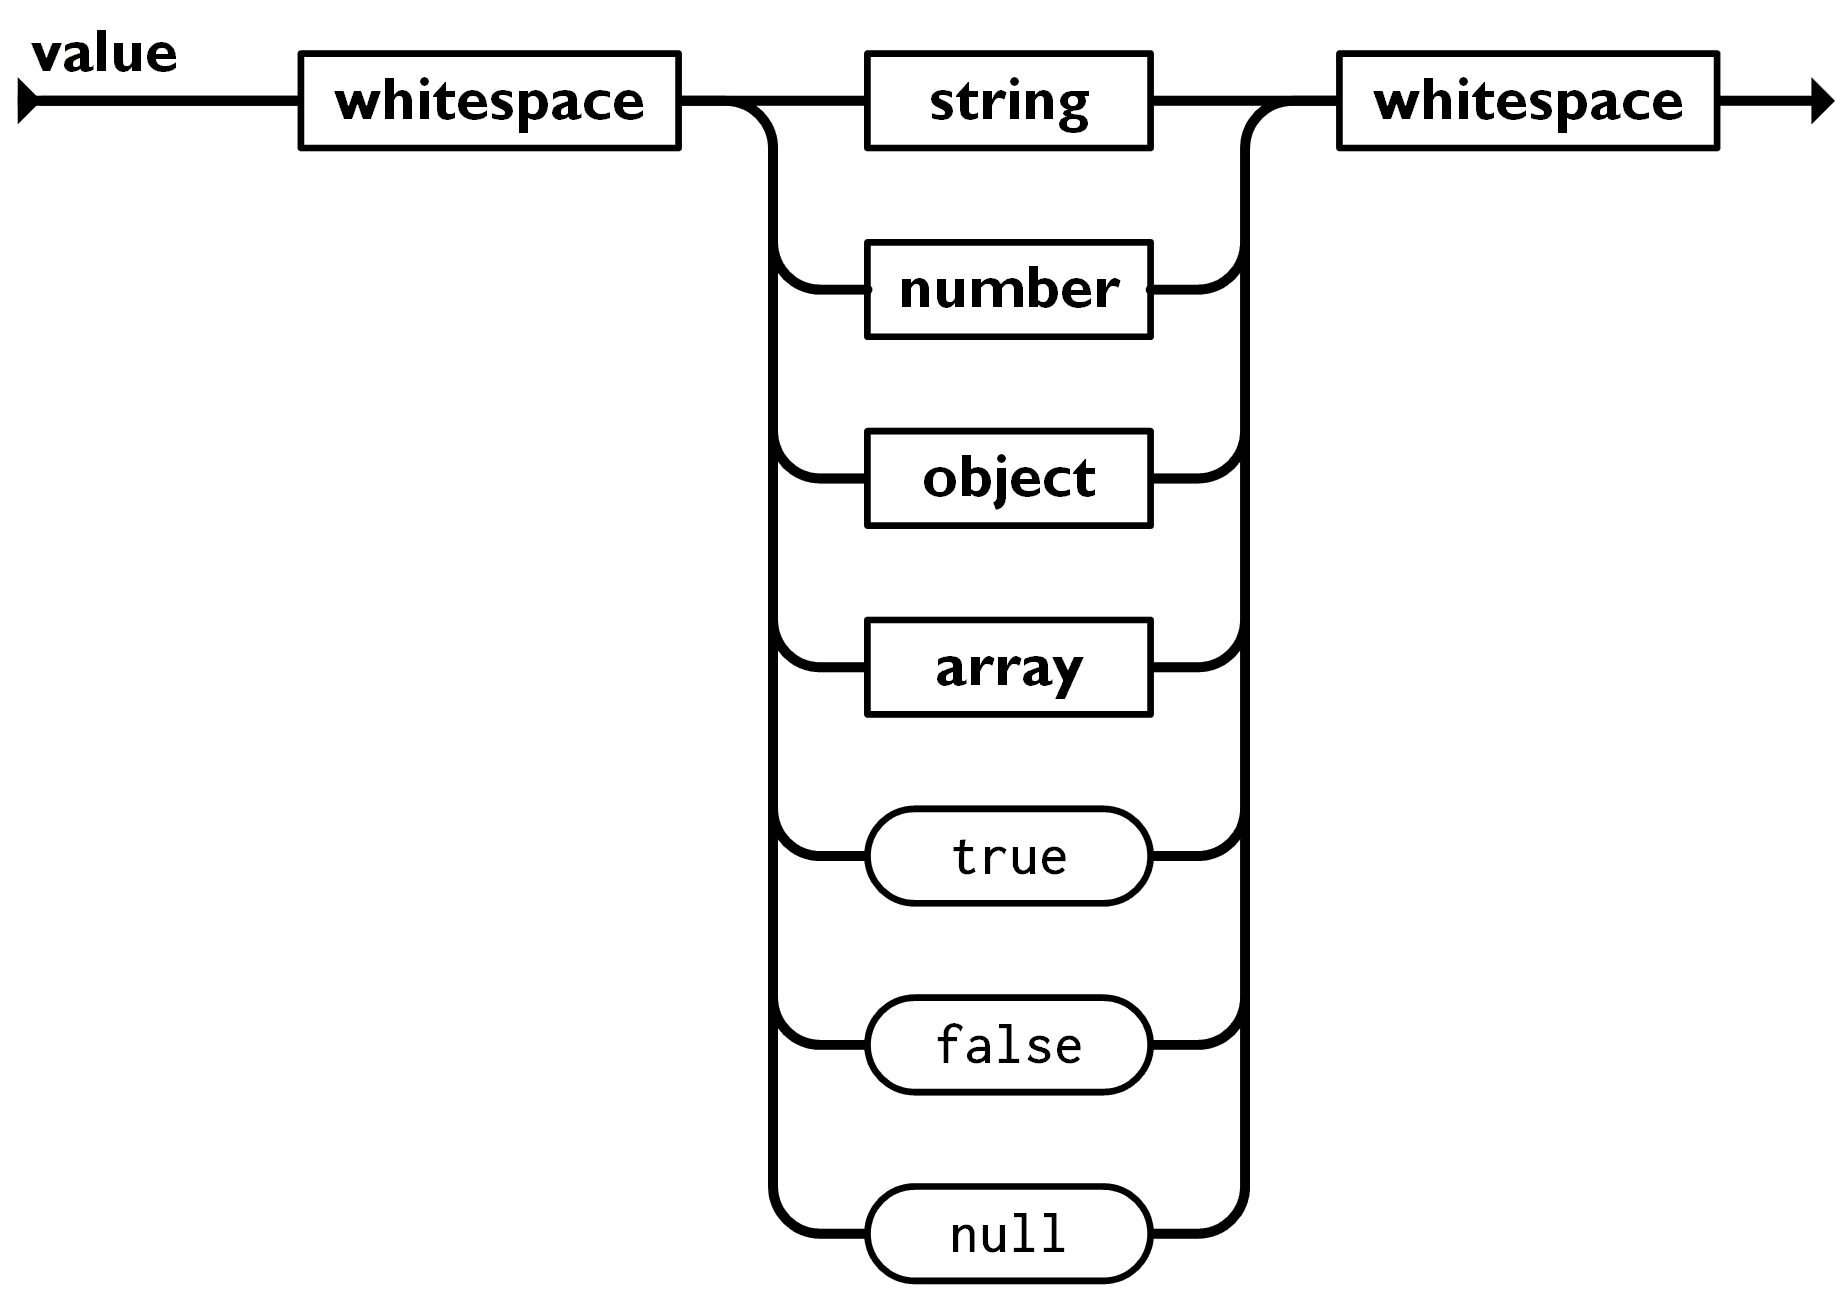
\includegraphics[width=10cm]{JSON_value}
		\caption{\acs{json} Value (Quelle: \url{https://www.json.org/img/value.png})  \label{fig:json_value}}
	\end{figure}
	
	\item \textbf{Objects} (\dt Objekte) sind ungeordnete Listen von beliebig vielen Name/Wert Paaren. Ein Name/Wert Paar besteht immer aus einem Namen, gefolgt von einem Doppelpunkt und dem zugehörigen Wert. Beistriche kommen zum Einsatz um Name/Wert Paare voneinander zu trennen. Ein Objekt wird immer von geschwungenen Klammern umschlossen. Der Aufbau eines \acs{json} Objekts ist in Abb.~\ref{fig:json_object} zu sehen.
	
	\begin{figure}[H]
		\centering
		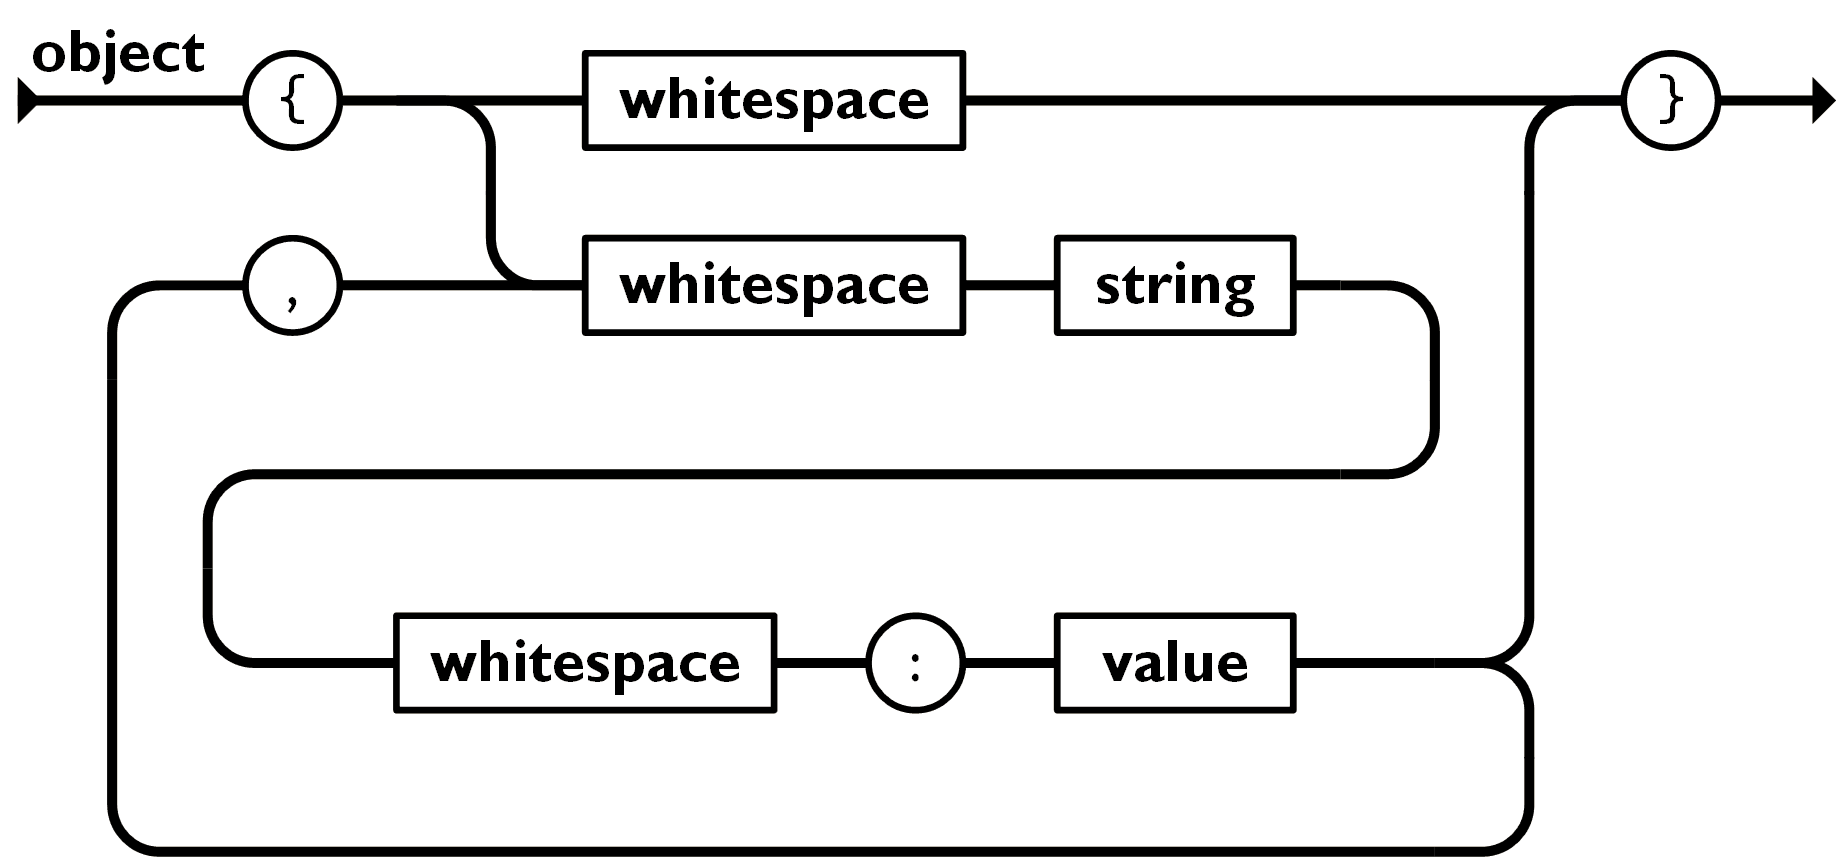
\includegraphics[width=10cm]{JSON_object}
		\caption{\acs{json} Object (Quelle: \url{https://www.json.org/img/object.png})  \label{fig:json_object}}
	\end{figure}
	
	\item \textbf{Arrays} sind geordnete Listen von Werten. Dabei werden Beistriche verwendet, um die Werte voneinander zu trennen. Ein Array wird immer von eckigen Klammern umschlossen. Der Aufbau eines Arrays ist in Abb.~\ref{fig:json_array} zu sehen.
	
	\begin{figure}[H]
		\centering
		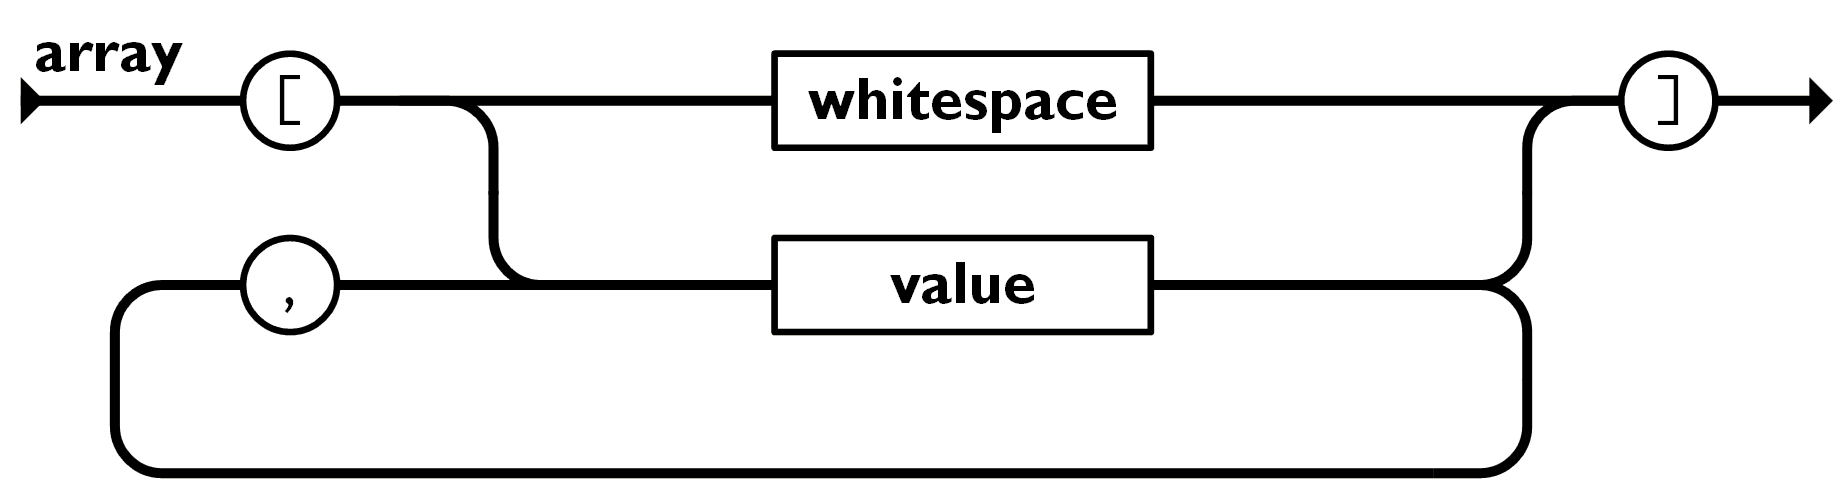
\includegraphics[width=10cm]{JSON_array}
		\caption{\acs{json} Array (Quelle: \url{https://www.json.org/img/array.png})  \label{fig:json_array}}
	\end{figure}
	
	\item \textbf{Strings} sind Zeichenketten. Sie können entweder leer sein, d. h. aus keinen Zeichen bestehen oder mehrere Unicode Zeichen enthalten. Eine Zeichenkette wird immer von Anführungszeichen umschlossen. Sie kann auch besondere Escapesequenzen beinhalten, die besondere Bedeutungen haben. Diese werden mit einem Backslash aufgerufen, wie \zB \enquote{\textbackslash n}, \enquote{\textbackslash t} oder \enquote{\textbackslash r}.
	
	\item \textbf{Numbers} (\dt Zahlen) sind numerische Werte, die aus einer oder mehreren dezimalen Ziffern bestehen. Sie können also keine Werte wie \zB \enquote{Infinity} oder \enquote{NaN} annehmen. Außerdem werden sie nie von Anführungszeichen umschlossen. 
	
\end{itemize}

Beispiele für \acs{json} Dateien sind in Kapitel \ref{json_config_files} zu finden.

\subsection{\acs{json} und \acs{csv} - Vergleich und Selektion} \label{json_vs_csv}
Sowohl \acs{json} als auch \acs{csv} bringen Vorteile mit sich. 
\acs{csv} Dateien können in Microsoft Excel bearbeitet und erstellt werden. Die tabellarische Darstellung und die Bekanntheit von Excel machen es zugänglich für Laien, was der größte Vorteil für \acs{csv} ist. Außerdem wird \acs{csv} von vielen Programmiersprachen unterstützt, was die Umsetzung theoretisch möglich machen würde. 

\acs{json} Dateien sind hingegen \acs{csv} zwar für Laien schwererer zu lesen, bieten aber hinsichtlich meist anderer Aspekte deutlich mehr Möglichkeiten. Anstatt des tabellarischen Aufbaus wird zum Speichern der Daten eine klare hierarchische Struktur verwendet. Die Struktur sorgt für mehr Flexibilität und eine besonders gute Darstellung verschachtelter Daten. Auch unterstützt \acs{json} unterschiedliche Datentypen, während bei \acs{csv} grundsätzlich nur Zeichenketten zum Einsatz kommen.

\acs{json} ist mittlerweile an Kompatibilität kaum zu übertreffen, was dessen Verwendung unbedenklich macht. Das Datenformat wird in unzähligen Bereichen eingesetzt und der Trend scheint immer weiter gegen \acs{json} zu gehen.

Schließlich überwiegen, im benötigten Anwendungsbereich, die vielen Vorteile von \acs{json} die schlechtere Leserlichkeit. Vor allem war die Möglichkeit der Verschachtelung der ausschlaggebende Grund weshalb sich für das \acs{json} Datenformat entschieden wurde. Dazu ist es wahrscheinlich, dass, wegen ihrem logischen Aufbau und  Skalierbarkeit, \acs{json} Dateien für den Anwendungszweck im Endeffekt übersichtlicher als \acs{csv} Dateien sind.

Falls bei Einführung der \acs{rltanzeige} Schwierigkeiten mit der Konfiguration auftreten steht \zB die Option eines Skripts, welches Excel Dateien in das gewünschte \acs{json} Format übersetzt, zur Verfügung.


\subsection{Dateikonzept} \label{json_config_files}
Für das Dateikonzept wurden drei Dateitypen auf Basis von \acs{json} Dateien entwickelt. Abbildung \ref{fig:vereinfachter_aufbau_dateikonzept} dient dem besseren Verständnis des Dateikonzepts. Hauptsächlich zeigt diese einen vereinfachten Aufbau der Komponenten, die von der Firma Bösch zur Entwicklung einer \acs{rltanzeige} bereitgestellt wurden, und die dazugehörigen Konfigurationsdateien. Die \acs{rltanzeige} selbst ist über den Bus mit einem Ventilator von ebm-papst sowie einem QBM9711 von Siemens verbunden. Der Ventilator verfügt lediglich über integrierte Sensorik. Der QBM9711 hingegen verfügt über zwei integrierte Luftdruck-Sensoren (interne Ports 1 und 2), zwei (an die Ports Analog Input 1 und 2) extern angeschlossene Temperatursensoren, eine (an den Port Analog Output 1) extern angeschlossene Klappe und ein (an den Port Analog Output 2) extern angeschlossenes Relais.


\begin{figure}[H]
	\centering
	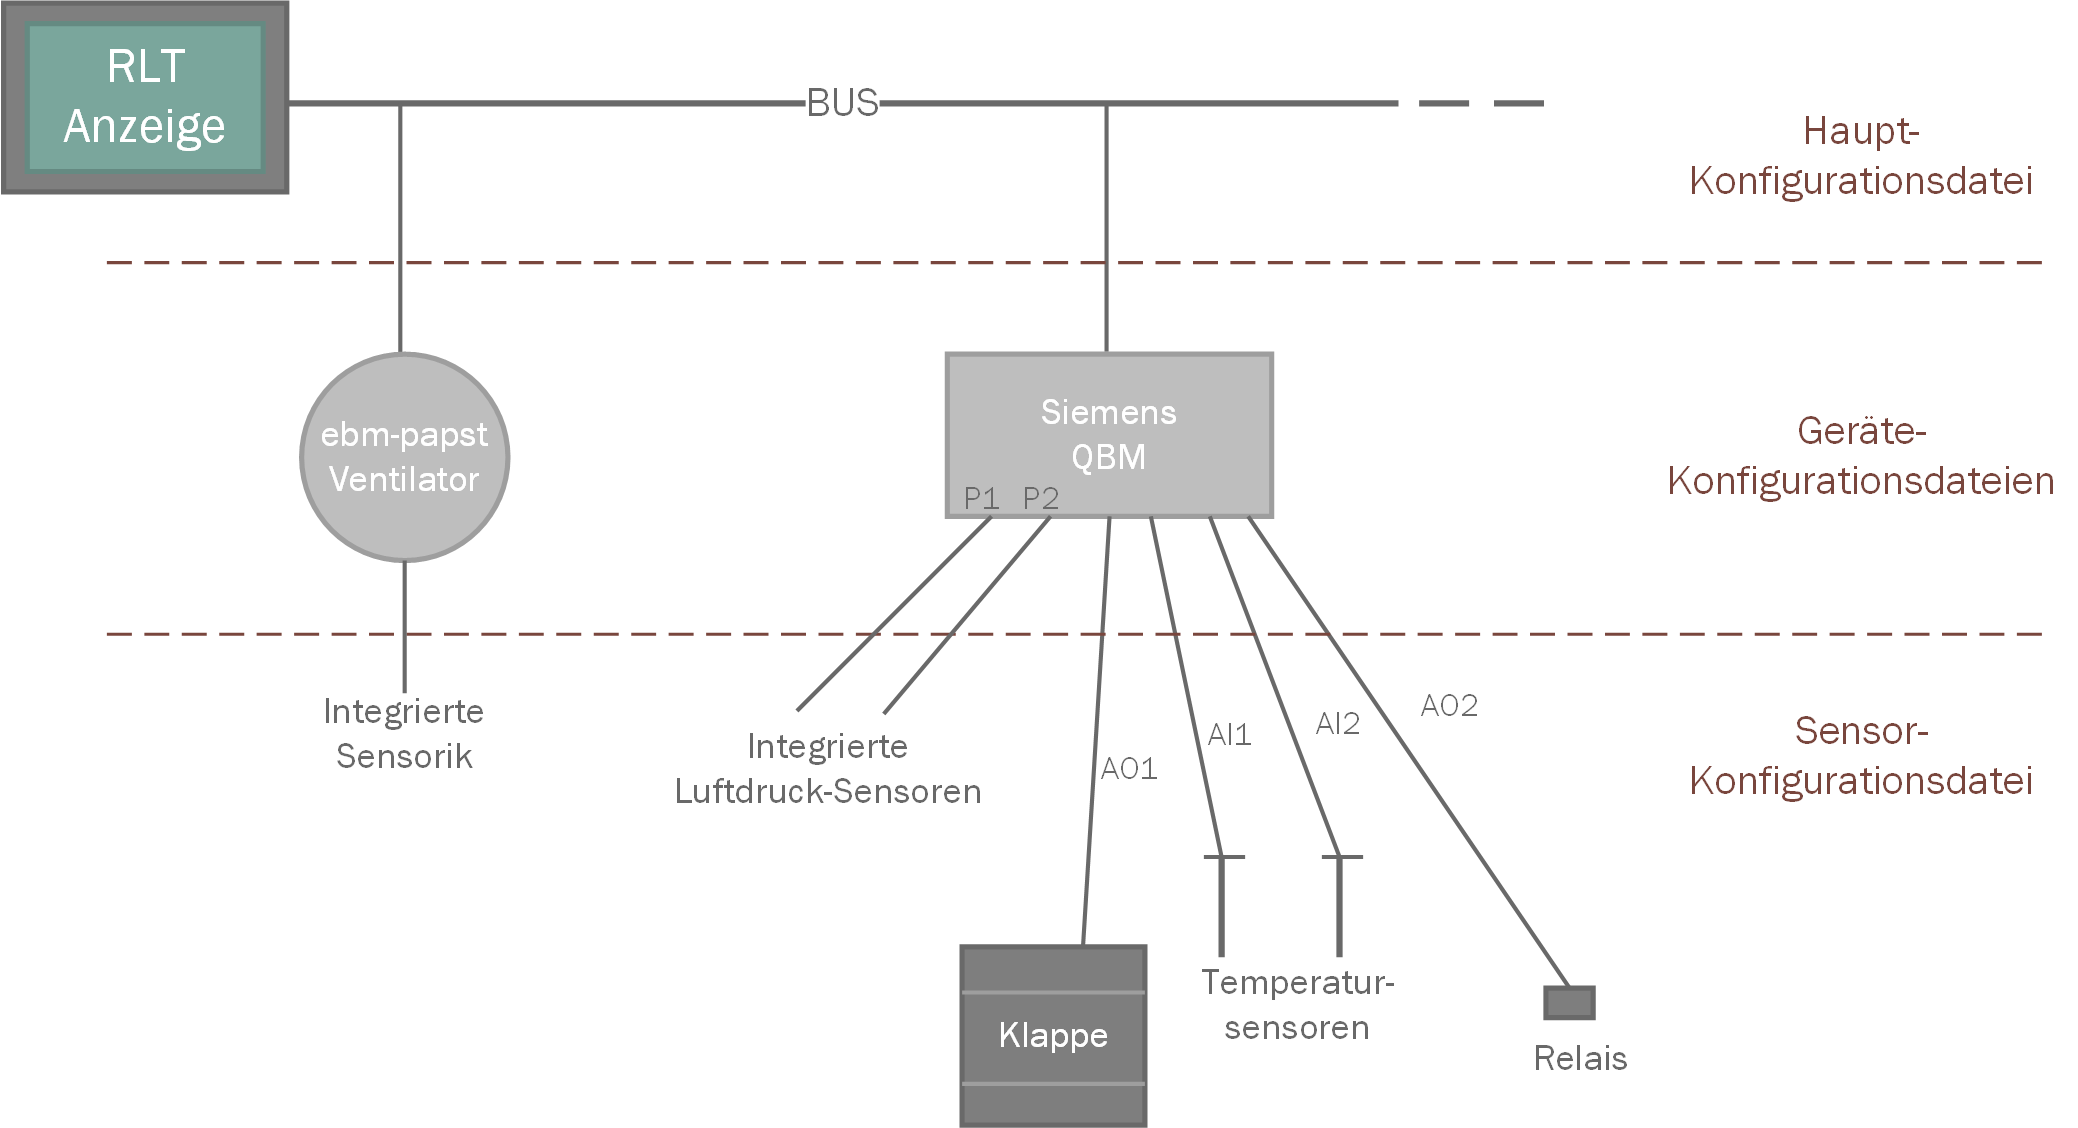
\includegraphics[width=\textwidth]{Komponenten_simpler_Aufbau_fuer_Dateikonzept}
	\caption{Vereinfachter Aufbau der Komponenten \label{fig:vereinfachter_aufbau_dateikonzept}}
\end{figure}

Es folgt eine aufbauende Beschreibung und Erklärung der drei Dateitypen:
%Fenkart fragen, ob ich bei den Geräten auf seinen Teil verweisen kann
% Wer beschreibt baud_rate, register, adresse, function code \ref{modbus_funktionsweise}

\begin{enumerate}

	\item \textbf{Sensor-Konfigurationsdatei} (\enquote{sensors.json}): Es gibt kein explizites Modbus Register, um die Maßeinheit eines Messwerts zu übertragen. Deswegen muss die Maßeinheit der unterschiedlichen Sensorik aus Datenblättern entnommen und jeweils zugeordnet werden. Dazu dient die Sensor-Konfigurationsdatei, welche eine Liste aller Sensoren (\zB bestimmte Temperatursensoren) mit der jeweils dazugehörigen Maßeinheit beinhaltet. Komponenten wie Ventilatoren haben integrierte Sensoren. Auch in diesem Fall kann für die Maßeinheit ein Eintrag in die \enquote{sensors.json} Datei gemacht werden. 
	
	Die einfache Ergänzung neuer Sensoren ist der Zweck der Sensor-Konfigurationsdatei. Diese muss nur dann verändert werden, wenn ein neuer Sensortyp, der noch nicht in der Sensor-Konfigurationsdatei steht, ergänzt wird. 
	
	Jeder Eintrag der Sensor-Konfigurationsdatei hat zwei Parameter, welche in Tab. \ref{tab:sensors_json_parameter} zu sehen sind.
		
	\begin{table}[h]
		\caption{Parameter der Sensor-Konfigurationsdatei (\enquote{sensors.json})}
		\label{tab:sensors_json_parameter}
		\begin{tabular}{p{\dimexpr 0.15\textwidth-2\tabcolsep} p{0.5\textwidth} | p{0.3\textwidth}}
			\toprule
			\textbf{Name} & \textbf{Beschreibung} & \textbf{Beispiel} \\
			\midrule
			type & Der Sensorname, auf den später in der Haupt-Konfigurationsdatei unter \enquote{type} referenziert wird. &  
			\begin{jsonTable}
"type": "NI1000"
			\end{jsonTable} 
 			\\
			unit & Die Einheit des entsprechenden Sensors. (Diese muss auch in der Geräte-Konfigurationsdatei unter \enquote{units} vorhanden sein.) &  
			\begin{jsonTable}
"unit": "°C"
			\end{jsonTable} 
			\\
			\bottomrule
		\end{tabular}
	\end{table}
	
		
	\item \textbf{Geräte-Konfigurationsdateien} (\zB \enquote{QBM97XX.json} oder \enquote{EBM.json}): Hier sind gerätespezifische Daten hinterlegt. Hauptsächlich welche Ausgabeports eine bestimmte Komponente (\zB ein Ventilator) besitzt, welche Einstellungen diese Ausgänge haben und \ggf welche Maßeinheiten die integrierten oder extern angeschlossenen Sensoren zurückgeben. 
	
	Weil in den \acs{rltanlagen} der Firma Bösch häufig die gleichen Komponenten verwendet werden, wurden spezielle Geräte-Konfigurationsdateien konzipiert. Diese Dateien können in der Haupt-Konfigurationsdatei beliebig oft referenziert werden, da sie einmalig für jedes Gerätemodell erstellt werden und nur selten Änderungen unterliegen. Das Hinzufügen einer neuen Geräte-Konfigurationsdatei ermöglicht zudem die einfache Integration einer neuen Komponente, beispielsweise eines Ventilators einer anderen Marke.
	
	Der Aufbau der Geräte-Konfigurationsdateien basiert auf einem \enquote{ports} Array. In dieses werden mithilfe der Parameter aus Tabelle \ref{tab:ports_array_parameter} die erforderlichen Informationen eingetragen.
	
	\begin{table}[H]
		\caption{Parameter des \enquote{ports} Array der Geräte-Konfigurationsdateien}
		\label{tab:ports_array_parameter}
		\begin{tabular}{p{\dimexpr 0.18\textwidth-2\tabcolsep} p{0.5\textwidth} | p{0.27\textwidth}}
			\toprule
			\textbf{Name} & \textbf{Beschreibung} & \textbf{Beispiel} \\
			\midrule
			port      	& Bezeichnung des Ausgabeports. Wird im Falle eines Geräts mit externer Sensorik (\zB Siemens QBM) in der Haupt-Konfigurationsdatei unter \enquote{port} referenziert. & 
			\begin{jsonTable}
"port": "AI1"
			\end{jsonTable} 
			\\
			register 	& Modbus Register (Erklärung in Kapitel \ref{modbus_funktionsweise}) in dem der jeweilige Messwert gespeichert ist \bzw welches ausgelesen werden soll. Das Register muss dabei immer dezimal angegeben werden, da minimalmodbus die hexadezimale Eingabe nicht unterstützt. & 
			\begin{jsonTable}
"register": 11
			\end{jsonTable} 
			\\
			function\_code 	& Modbus Function Code (Erklärung in Kapitel \ref{modbus_funktionsweise}), mit dem auf das vorher angegebene Register zugegriffen werden soll. Die zwei meist verwendeten Function Codes sind \enquote{3} für Input Register und \enquote{4} für Holding Register. & 
			\begin{jsonTable}
"function_code": 3
			\end{jsonTable} 
			\\
			units 	& Array in dem jeder möglichen Maßeinheit für den jeweiligen Ausgabeport eine Skalierung zugeordnet wird. Die Skalierung dient \zB dazu, dem Messwert die angemessene Anzahl von Dezimalstellen zuzuweisen, da diese über Modbus nicht übertragen werden (Funktionsweise in Kapitel \ref{auslesen_rlt_parameter} erklärt).
			
			Wird bei Ports weggelassen, deren Werte nur von Python Funktionen (Erklärung in Kapitel \ref{python_functions}) zur Weiterverarbeitung verwendet werden.
			
			Die Parameter eines Objekts dieses Arrays sind in Tabelle \ref{tab:units_array_parameter} zu sehen.  & 
			\begin{jsonTable}
"units": "[ ]"
			\end{jsonTable} 
			\\
			\bottomrule
		\end{tabular}
	\end{table}
	
	
	
	\begin{table}[H]
		\caption{Parameter des Unterarray \enquote{units}}
		\label{tab:units_array_parameter}
		\begin{tabular}{p{\dimexpr 0.18\textwidth-2\tabcolsep} p{0.47\textwidth} | p{0.3\textwidth}}
			\toprule
			\textbf{Name} & \textbf{Beschreibung} & \textbf{Beispiel} \\
			\midrule
			unit      	& Die Maßeinheit, die aus der Sensor-Konfigurationsdatei referenziert wird. & 
			\begin{jsonTable}
"unit": "°C"
			\end{jsonTable} 
			\\
			scaling 	& Skalierung des Messwertes. Kann aus Datenblättern entnommen werden. & 
			\begin{jsonTable}
"scaling": 0.1
			\end{jsonTable} 
			\\
			\bottomrule
		\end{tabular}
	\end{table}
		
	\item \textbf{Haupt-Konfigurationsdatei} (\enquote{main\_config\_file.json}):
	Wie in Kapitel \ref{gui_design} beschrieben, ist zur übersichtlichen Darstellung der Messwerte eine Aufteilung in mehrere Abschnitte bzw. Seiten erforderlich. Auf diesen Seiten werden jeweils sinngemäß Messwerte zusammengefasst. Die Konfiguration der Seiten erfolgt in der Haupt-Konfigurationsdatei mithilfe von zwei parallelen Arrays: dem \enquote{pages}-Array und dem \enquote{devices}-Array. 	
	
	Im \enquote{devices} Array werden die alle Komponenten \bzw Quellen der \acs{rltanlage}, nämlich Ventilatoren und QBMs (vgl. Abb. \ref{fig:vereinfachter_aufbau_dateikonzept}), aufgeführt, von denen Messwerte ausgelesen werden sollen. Die Parameter des \enquote{devices} Arrays sind in Tabelle \ref{tab:devices_array_parameter} näher erläutert.
	
	\begin{table}[H]
		\caption{Parameter des \enquote{devices} Array der Haupt-Konfigurationsdatei}
		\label{tab:devices_array_parameter}
		\begin{tabular}{p{\dimexpr 0.17\textwidth-2\tabcolsep} p{0.48\textwidth} | p{0.3\textwidth}}
			\toprule
			\textbf{Name} & \textbf{Beschreibung} & \textbf{Beispiel} \\
			\midrule
			device     	& Angabe des Gerätetyps, indem auf den Namen der zugehörigen Geräte-Konfigurationsdatei referenziert wird. & 	
			\begin{jsonTable}
"device": "QBM97XX"
			\end{jsonTable}  
			\\
			id         	& Beliebig auswählbare, jedoch eindeutige Bezeichnung für das Gerät. Mit der \enquote{id} wird im \enquote{pages} Array auf das Gerät referenziert.  & 	
			\begin{jsonTable}
"id": "QBM1"
			\end{jsonTable}  
			\\
			baud\_rate	& Eingestellte Baudrate. Ist bei allen Komponenten einer \acs{rltanlage} gleich. & 	
			\begin{jsonTable}
"baud_rate": 19200
			\end{jsonTable}  
			\\
			mbaddress	& Die Modbus Adresse des Geräts. (vgl. Kapitel \ref{modbus_funktionsweise}) & 	
			\begin{jsonTable}
"mbaddress": 1
			\end{jsonTable}  
			\\
			parity	& Parität. Mögliche Werte: \enquote{even}, \enquote{odd} oder \enquote{none} (vgl. Kapitel \ref{modbus_uebertragungsarten}) & 	
			\begin{jsonTable}
"parity": "even"
			\end{jsonTable}  
			\\
			stop\_bits	& Anzahl der Stopbits einer Nachricht (vgl. Kapitel \ref{modbus_uebertragungsarten}) & 	
			\begin{jsonTable}
"stop_bits": 1
			\end{jsonTable}  
			\\
			zero\_based	& Gibt an, ob die Modbus Register von 0 oder 1 ausgehend gezählt werden. Mögliche Werte: \enquote{true} oder \enquote{false}.
			
			(Bemerkung: Bei Siemens QBMs normalerweise \enquote{false}, bei ebm-papst Ventilatoren \enquote{true}) & 	
			\begin{jsonTable}
"zero_based": false
			\end{jsonTable}  
			\\
			sensors	& Array aller am Gerät angeschlossenen Sensoren. Bei Ventilatoren und Ausgabeports, deren Werte ausschließlich von Python Funktionen zur Weiterverarbeitung genutzt werden (Erklärung in Kapitel \ref{python_functions}), wird auf die Angabe verzichtet. 
			
			Die zwei Parameter, die für jedes Objekt dieses Arrays angegeben werden, sind in Tabelle \ref{tab:sensors_array_parameter} zu finden. & 	
			\begin{jsonTable}
"sensors": [ ]
			\end{jsonTable}  
			\\
			\bottomrule
		\end{tabular}
	\end{table} 
	
	\begin{table}[H]
		\caption{Parameter des Unterarray \enquote{sensors}}
		\label{tab:sensors_array_parameter}
		\begin{tabular}{p{\dimexpr 0.18\textwidth-2\tabcolsep} p{0.45\textwidth} | p{0.32\textwidth}}
			\toprule
			\textbf{Name} & \textbf{Beschreibung} & \textbf{Beispiel} \\
			\midrule
			port   	& Verweist auf den Ausgabeport aus der Geräte-Konfigurationsdatei (siehe Tab. \ref{tab:ports_array_parameter}). Mögliche Werte können also \zB der Datei \enquote{QBM97XX.json} entnommen werden. & 	
			\begin{jsonTable}
"port": "AI1"
			\end{jsonTable}  
			\\
			type 	& Verweist auf einen Sensor aus der Sensor-Konfigurationsdatei. Mögliche Werte können also \zB der Datei \enquote{sensors.json} entnommen werden. & 	
			\begin{jsonTable}
"type": "LG-NI1000"
			\end{jsonTable}  
			\\
			\bottomrule
		\end{tabular}
	\end{table}
	

	Im \enquote{pages} Array werden alle Seiten, die später auf der \acs{rltanzeige} veranschaulicht werden sollen, definiert. Dabei werden die in Tabelle \ref{tab:devices_array_parameter} definierten Quellen den richtigen Seiten zugeordnet. Die Parameter des \enquote{pages} Array sind in Tabelle \ref{tab:pages_array_parameter} notiert.
	
	% unterschiedliche anzahl der Komponenten

	\begin{table}[H]
		\caption{Parameter des \enquote{pages} Array der Haupt-Konfigurationsdatei}
		\label{tab:pages_array_parameter}
			\begin{tabular}{p{\dimexpr 0.15\textwidth-2\tabcolsep} p{0.45\textwidth} | p{0.35\textwidth}}
			\toprule
			\textbf{Name} & \textbf{Beschreibung} & \textbf{Beispiel} \\
			\midrule
			title      	& Beliebig auswählbarer Titel der Seite. & 
			\begin{jsonTable}
"title": "Allgemein"
			\end{jsonTable} 
			\\
			sources 	& Array aller Messwerte, die auf einer Seite angezeigt werden sollen. Die Parameter, die in einem Objekt dieses Arrays benutzt werden, sind in Tab. \ref{tab:sources_array_parameter} zu sehen. & 
			\begin{jsonTable}
"sources": "[ ]"
			\end{jsonTable} 
			\\
			\bottomrule
		\end{tabular}
	\end{table}
	
	\begin{table}[H]
		\caption{Parameter des Unterarray \enquote{sources}}
		\label{tab:sources_array_parameter}
			\begin{tabular}{p{\dimexpr 0.2\textwidth-2\tabcolsep} p{0.42\textwidth} | p{0.33\textwidth}}
			\toprule
			\textbf{Name} & \textbf{Beschreibung} & \textbf{Beispiel} \\
			\midrule
			port                & Ein Array mit den Quellen, aus denen der Messwert ausgelesen wird. Dabei wird meistens nur ein Objekt mit \enquote{id} (siehe Tab. \ref{tab:devices_array_parameter}) des Geräts und \enquote{port} (siehe Tab. \ref{tab:ports_array_parameter}) angegeben. In einigen Szenarien ist es erforderlich, mehrere Quellen für abgeleitete Messwerte zu verwenden (siehe Kapitel \ref{python_functions}). In solchen Fällen werden dem Array zusätzliche Objekte hinzugefügt. &  
			\begin{jsonTable}
"port": [
	{ "QBM1": "AI1" }
]
			\end{jsonTable} 
			\\
			description         & Beliebig auswählbare Bezeichnung für den Messwert. Der Messwert wird später auf der \acs{rltanzeige} so bezeichnet. & 
			\begin{jsonTable}
"description": "Temperatur Zuluft"
			\end{jsonTable}  
			\\
			python\_function    & (Optionaler) Parameter, der nur angegeben wird, wenn der jeweilige Messwert abgeleitet berechnet werden muss. (Erklärung in Kapitel \ref{python_functions}). & 
			\begin{jsonTable}
"python_function": "relay_position"
			\end{jsonTable} 
			\\
			additional\_info    & (Optionaler) Parameter, der nur angegeben wird, falls die jeweilige Python Funktion zusätzliche Informationen benötigt. (Erklärung in Kapitel \ref{python_functions}). & 
			\begin{jsonTable}
"additional_info": { "switching_voltage": 5 }
			\end{jsonTable} 
			\\
			\bottomrule
		\end{tabular}
	\end{table} 
					
\end{enumerate}

%Bedienungsanleitung für Servicetechniker erwähnen
Zuletzt ist zu erwähnen, dass Servicetechnikerinnen und Servicetechniker zur Installation einen Ordner bekommen. Darin befindet sich direkt eine Vorlage für die \enquote{main\_config\_file.json} Datei, welche im Normalfall die einzige Datei sein sollte, die bearbeitet bzw. verändert wird.
In einem Unterordner (\enquote{devices}) sind Geräte-Konfigurationsdateien und die Sensor-Konfigurationsdatei zu finden. Diese Dateien müssen, wie gerade erwähnt, nur verändert werden, wenn noch nie verwendete Komponenten, wie z.B. eine neue Art von Ventilator oder Sensor, in der \acs{rltanlage} verbaut werden.

Ein Beispiel zu allen Dateitypen ist im Anhang zu finden.






\setAuthor{\schneider}
\subsection{Einlesen der Konfigurationsdateien} \label{einlesen_konfigurationsdateien}
\paragraph{Klassenstruktur}
Im Backend wird die Klassenstruktur der \ac{gui} nachgebildet. Es gibt eine \lstinline{Page}, eine \lstinline{Measurement} und eine \lstinline{Sensor} Klasse. Eine \lstinline{Measurement} Instanz kann mehrere \lstinline{Sensor} Instanzen enthalten, da manche \lstinline{Measurements} zur Berechnung (z.B. der Wärmerückgewinnungsgrad) mehrere Messwerte benötigen. Die \lstinline{Page} Instanzen speichern die jeweiligen \lstinline{Measurement} Instanzen, die auf dieser Seite angezeigt werden sollen. Die \lstinline{Page} Instanzen existieren, damit der ausgelesene Parameter an der richtigen Stelle auf der \acs{gui} verändert werden kann. Es gibt nämlich gleich viele \lstinline{Page} Instanzen wie \lstinline{PageFrame} Instanzen (vgl. Kapitel \ref{tkintercode}) und gleich viele \lstinline{Measurement} Instanzen wie \lstinline{MeasurementFrame} Instanzen. (siehe Abb.~\ref{fig:uml_backend}).
\begin{figure}[ht]
	\centering
	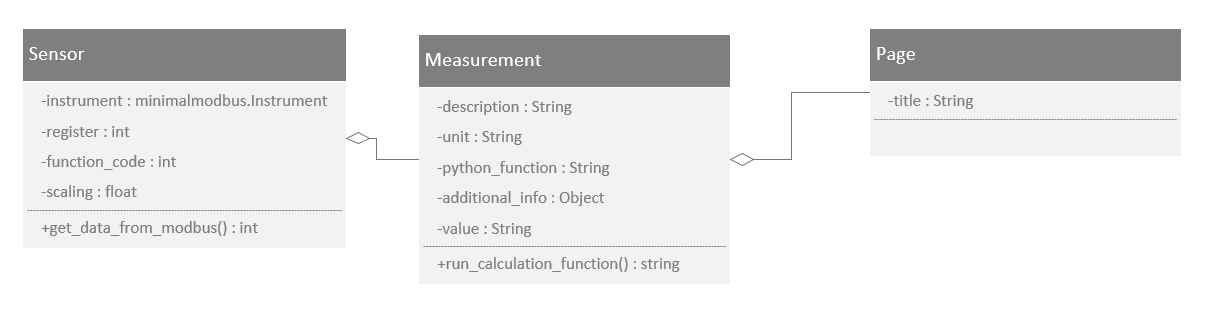
\includegraphics[width=1.0\linewidth]{Bilder/UML_Backend}
	\caption{UML Diagramm Backend}
	\label{fig:uml_backend}
\end{figure}

Die \lstinline{Page}, \lstinline{Measurement} und \lstinline{Sensor} Instanzen werden beim Einlesen der \acs{json} Konfigurationsdateien aufgrund der Objekte im \enquote{pages}  Array (vgl. Kapitel \ref{json_config_files}) erstellt und in Listen gespeichert. \newline
Zum Einlesen werden drei Funktionen implementiert:
\begin{itemize}
	\item \textbf{\lstinline{load_config()}:} Diese Funktion lädt die gesamte Haupt-Konfigurationsdatei ein. Es werden die angeschlossenen Geräte ermittelt und die \lstinline{Page}, \lstinline{Measurement} und \lstinline{Sensor} Instanzen erstellt. Dafür kommen die beiden folgenden Hilfsfunktionen zum Einsatz.
    \begin{itemize}
		\item \textbf{\lstinline{get_sensor_unit()}:} Liest die Sensor-Konfigurationsdateien ein. Dadurch können den Messwerten die richtigen Maßeinheiten zugewiesen werden.
		\item \textbf{\lstinline{get_sensor_data()}:} Liest aus der Geräte-Konfigurationsdatei am angegebenen Port die Parameter aus und liefert diese Parameter als \acs{json} Objekt zurück. Sie liest das Register, den \gls{modbus} Function Code und die Skalierung aus. Die Skalierung wird anhand der Maßeinheit aus der Sensor-Konfigurationsdatei ausgewählt.
	\end{itemize}
\end{itemize}

\paragraph{Einlesen und Erstellen der Instanzen}
Einlesen kann man ein \acs{json} Attribut mit folgender Syntax. Im folgenden Beispiel wird aus der Instanz namens \lstinline{page} das Attribut \enquote{title} gesucht und zurückgeliefert.
\begin{pythoncode}
title = page["title"]
\end{pythoncode}

Im folgenden Code werden die \lstinline{Measurement} Instanzen erstellt, indem die anzuzeigenden Messwerte aus dem \enquote{sources} Array iteriert werden. Anhand der Informationen der Objekte im \enquote{sources} Array werden dann die entsprechenden Geräte im \enquote{devices} Array herausgesucht. Es werden weitere Parameter aus der Haupt-Konfigurationsdatei ausgelesen, die zu dem entsprechenden Messwert gehören (z.B. die Bezeichnung oder die Einheit). Anschließend werden die \lstinline{Sensor} Instanzen erstellt und einer Liste beigefügt, da manche Measurements (z.B. die Rückwärmzahl) mehrere Messwerte benötigen. Diese Liste, sowie die vorher ausgelesenen Parameter werden beim Erstellen der \lstinline{Measurement} Instanzen dem Konstruktor übergeben und darin in Instanzvariablen gespeichert.
\begin{pythoncode}
page_measurements = []
for measurements in page["sources"]:
	measurements_sensors = []
	#[Auslesen weiterer Parameter der Haupt-Konfigurationsdatei (description, unit, python_function,additional_info)]
	#[Erstellen der Sensor Instanzen (Siehe nächster Codeblock)]
	page_measurements.append(Measurement(description=description, unit=unit, sensors=measurements_sensors, python_function=python_function, additional_info=additional_info))
\end{pythoncode}

Im folgenden Code wird für jeden Port (an jedem Port ist ein \lstinline{Sensor} angeschlossen) eines Geräts eine \lstinline{Sensor} Instanz erstellt. Alle \lstinline{Sensor} Instanzen werden der \lstinline{page_sensors} Liste beigefügt. Dafür gibt es im \enquote{sources} Array die einzelnen Ports. Das sind Wertepaare, die jeweils aus Gerät und \lstinline{Sensor} bestehen (vgl. Kapitel \ref{json_config_files}). Mit diesen beiden Werten kann dann das entsprechende Gerät im \enquote{devices} Array gefunden werden und darin der entsprechende Port im \enquote{sensors} Array. Mit der \lstinline{get_sensor_unit()} Funktion wird die Einheit erhalten und mit der \lstinline{get_sensor_data()} Funktion weitere Sensordaten. Diese werden beim Erstellen der \lstinline{Sensor} Instanz dem Konstruktor übergeben.
\begin{pythoncode}
port_counter = 0
for port in port_arr:
	device_id = list(port.keys())[port_counter] # example: QBM1
	port_id = port[device_id]  # example: AI1
	port_counter += 1
	
	for device in config_full_data[0]["devices"]:
		if device["id"] == device_id:
			#[Aufruf der get_sensor_unit Funktion]
			#[Auslesen der Geräteparameter in der Haupt-Konfigurationsdatei (baud_rate, mbaddress etc.)]
			#[Aufruf der get_sensor_data Funktion]
			measurements_sensors.append(Sensor(baud_rate=device["baud_rate"], ..., register=register, zero_based=device["zero_based"]))
\end{pythoncode}

Die \lstinline{Measurement} Instanzen sind nach dem Erstellen alle in einer Liste gespeichert. Zum Schluss werden \lstinline{Page} Instanzen erstellt. Die \lstinline{Measurement} Liste wird so aufgeteilt, dass maximal 5 Measurements auf einer Seite sind. Anhand dieser \lstinline{Page}- und \lstinline{Measurement} Instanzen wird beim Erstellen der \acs{gui} die Anzahl an Seiten übernommen, der Seitentitel und die Beschreibungen der Messwerte gesetzt (siehe Kapitel \ref{gui_design}). 
\begin{pythoncode}
counter = 0
last_slice = 0
for measurement in page_measurements:
	counter += 1
	if ((counter % 5) == 0) or (counter == len(page_measurements)):
		all_pages.append(Page(title=title, measurements=page_measurements[last_slice:counter]))
		last_slice = counter
\end{pythoncode}

%\pythonfile[firstline=125, lastline=197]{Code/modbus.py}

Im Konstruktor der \lstinline{Page}, \lstinline{Measurement} und \lstinline{Sensor} Klasse werden die ausgelesenen Variablen in Instanzvariablen gespeichert.

\section{Python Funktionen}
\setAuthor{\pezze}
\label{python_functions}
Messwerte werden aus Modbus Registern der unterschiedlichen Komponenten einer \acs{rltanlage} bezogen.  Grundsätzlich wird jeder ausgelesene Wert direkt auf der \acs{rltanzeige} angezeigt, wobei Skalierung und Maßeinheit hinzugefügt werden. In einigen Fällen muss jedoch ein Wert aus mehreren Messwerten abgeleitet werden, eine spezielle Umrechnung oder Ähnliches erfolgen, bevor der Wert auf der \acs{rltanzeige} dargestellt werden kann. In einem solchen Fall wird in der Haupt-Konfigurationsdatei im \enquote{pages} Array (vgl. Kapitel \ref{json_config_files}) der Name einer Python Funktion angegeben, die ausgeführt werden muss, um den erwünschen Wert zu erhalten. 

Diese Python Funktionen sind in der Datei \enquote{modbus\_functions.py} definiert, was den folgenden Vorteil bietet: Ein einfaches Hinzufügen neuer Komponenten, deren Messwerte abgeleitet werden müssen, ohne dass der restliche Code verändert werden muss. Bei der Integration einer neuen Komponente werden lediglich die nötigen Funktionen in der \enquote{modbus\_functions.py} Datei hinzugefügt und diese folgend in der Haupt-Konfigurationsdatei referenziert. Dies ermöglicht eine flexible  Erweiterung des Systems.

Eine solche Python Funktion hat den folgenden grundlegenden Aufbau:
\begin{pythoncode}
def Funktionsname(sensors, additional_info):
	...	
	return Ergebnis
\end{pythoncode}

Jede Funktion erwartet die Übergabeparameter \enquote{sensors} und \enquote{addictional\_info}. \enquote{sensors} ist eine Liste, die Objekte der Klasse \enquote{Sensor} beinhaltet. Ein Objekt der Klasse \enquote{Sensor} wiederum enthält alle erforderlichen Informationen, um einen Wert aus einem Modbus Register auszulesen, wie es in Kapitel \ref{auslesen_rlt_parameter} beschrieben wird. \newline 
Der Parameter \enquote{additional\_info} ermöglicht die Übermittlung weiterer Informationen, falls diese bei der Berechnung oder Ableitung der Werte benötigt werden.

Im folgenden Abschnitt werden die bisher definierten Python Funktionen beschrieben, eine weitere Erklärung zum Ablauf bei der Ausführung der Python Funktionen ist in Kapitel \ref{auslesen_rlt_parameter} zu finden.


\paragraph{Funktion \enquote{standard}}
Diese Funktion wird standardmäßig ausgeführt, wenn in der Haupt-Konfigurationsdatei (vgl. Kapitel \ref{json_config_files}) der Parameter \enquote{python\_function} nicht angegeben wird \bzw keine besondere Python Funktion angegeben wird. Die \enquote{standard} Funktion wird daher als einzige dieser Funktionen nie direkt in der Haupt-Konfigurationsdatei referenziert.

Wie im unten stehenden Code zu sehen ist, wird bei dieser Funktion nichts berechnet. Es wird lediglich die \enquote{get\_data\_from\_modbus} Funktion der \enquote{Sensor} Instanz aufgerufen, welche den Messwert aus dem jeweiligen Modbus Register ausliest und zurück gibt (weitere Erklärung in Kapitel \ref{auslesen_rlt_parameter}).

\begin{pythoncode}
def standard(sensors, additional_info):
	return sensors[0].get_data_from_modbus()
\end{pythoncode}


\paragraph{Funktion \enquote{calc\_rpm}}
Wird verwendet, um bei ebm-papst Ventilatoren die Soll- \bzw Ist-Drehzahl zu ermitteln. Dabei werden, wie im folgenden Code zu sehen ist, zwei Register ausgelesen. Daraufhin wird das Verhältnis der jeweiligen Drehzahl zur maximalen Drehzahl des Ventilators berechnet, das Ergebnis gerundet und in Prozent zurückgegeben.

\begin{pythoncode}
def calc_rpm(sensors, additional_info):
	max_value = sensors[1].get_data_from_modbus()
	rpm_value = (sensors[0].get_data_from_modbus() / 64000) * max_value
	ratio = rpm_value / max_value * 100.0
	return str(round(ratio, 1)) + " %"
\end{pythoncode}

Die Gleichung \eqref{glg:drehzahl_berechnung} für die Berechnung des Wertes \enquote{rpm\_value} stammt aus dem Datenblatt für ebm-papst Ventilatoren \cite[vgl.][118,122]{ebmpapst:2020}: 
\begin{equation}
	\text{rpm\_value}\left[\frac{1}{min}\right] = \frac{\text{Datenbytes}}{64000} \cdot \text{max\_value} \left[\frac{1}{min}\right]
	\label{glg:drehzahl_berechnung}
\end{equation} 

Eine Angabe in der Haupt-Konfigurationsdatei sieht wie folgt aus. Dabei ist zu sehen, dass im \enquote{port} Array zuerst die Quelle der Ist- \bzw Soll-Drehzahl (\enquote{RPMreal} \bzw \enquote{RPMtarget})und als zweites die Quelle der maximalen Drehzahl (\enquote{RPMmax}). Es wird keine \enquote{additional\_info} angegeben.

\begin{jsoncode}
"sources": [
	{
		"port": [
			{"EBM1": "RPMreal"},
			{"EBM1": "RPMmax"}
		],
		"description": "Drehzahl Istwert",
		"python_function": "calc_rpm"
	},
	...
]
\end{jsoncode}



\paragraph{Funktion \enquote{calc\_power}}
Wird verwendet, um den Leistungsverbrauch von ebm-papst Ventilatoren zu ermitteln. Dabei werden, wie im folgenden Code zu sehen ist, drei Register ausgelesen und mit diesen der Leistungsverbrauch berechnet. Daraufhin wird das Ergebnis gerundet und mit der Maßeinheit \enquote{$W$} zurückgegeben.

\begin{pythoncode}
def calc_power(sensors, additional_info):
	byte_value = sensors[0].get_data_from_modbus()
	Uz_value = sensors[1].get_data_from_modbus() / 1000 * 20
	Iz_value = sensors[2].get_data_from_modbus() / 1000 * 2
	power = (byte_value / 65536) * Uz_value * Iz_value
	return str(round(power, 1)) + " W"
\end{pythoncode}

Für die Berechnung des aktuellen Leistungsverbrauchs wurden folgende Gleichungen \eqref{glg:calc_power} \eqref{glg:calc_uz} \eqref{glg:calc_iz} aus dem Datenblatt für ebm-papst Ventilatoren abgeleitet \cite[vgl.][95,126]{ebmpapst:2020}: 
\begin{equation}
	\text{Uz\_value} \left[V\right] = \frac{\text{byte\_value} * 20 \left[mV\right]}{1000}
	\label{glg:calc_uz}
\end{equation} 
\begin{equation}
	\text{Iz\_value} \left[A\right] = \frac{\text{byte\_value} * 2 \left[mA\right]}{1000}
	\label{glg:calc_iz}
\end{equation} 

\begin{equation}
	\text{power} \left[W\right] = \frac{\text{byte\_value}}{65536} \cdot \text{Uz\_value}  \left[V\right] \cdot \text{Iz\_value} \left[A\right]
	\label{glg:calc_power}
\end{equation} 

Eine Angabe in der Haupt-Konfigurationsdatei sieht wie folgt aus. Dabei ist zu sehen, dass im \enquote{port} Array zuerst die Quelle \enquote{Power}, als zweites die Quelle \enquote{Uz} und zuletzt die Quelle \enquote{Iz} eines ebm-papst Ventilators angegeben werden. Es wird keine \enquote{additional\_info} angegeben.

\begin{jsoncode}
"sources": [
	{
		"port": [
			{"EBM1": "Power"},
			{"EBM1": "Uz"},
			{"EBM1": "Iz"}
		],
		"description": "Leistung",
		"python_function": "calc_power"
	},
	...
]
\end{jsoncode}



\paragraph{Funktion \enquote{eng\_status}}
Wird verwendet, um bei ebm-papst Ventilatoren den Motorstatus \bzw aktuelle Fehlermeldungen zu ermitteln. Dabei wird, wie im folgenden Code zu sehen ist, ein Register ausgelesen, worin ein Statuscode enthalten ist. Daraufhin wird dieser Statuscode in eine binäre Zeichenkette konvertiert und seine einzelnen Bits analysiert. Falls ein Bit den Wert \enquote{1} hat, wird zur Zeichenkette \enquote{error\_string} der Fehlercode angehängt. Die Zeichenkette \enquote{error\_string} wird zuletzt zurückgegeben und kann mithilfe des Datenblatt für ebm-papst Ventilatoren \cite[vgl.][119]{ebmpapst:2020} entziffert werden. 

\begin{pythoncode}
def eng_status(sensors, additional_info):
	status = sensors[0].get_data_from_modbus()
	binary_status = bin(status)
	error_string = ""
	counter = 0
	for s in reversed(binary_status):
		counter += 1
		if s == "1":
			if counter == 1:
				error_string += "PHA "
			...
			elif counter == 13:
				error_string += "UzLow "
			else:
				error_string += "Unbekannter Fehler"
			
	if error_string == "":
		error_string = "Kein Fehler"
	
	return error_string
\end{pythoncode}

Eine Angabe in der Haupt-Konfigurationsdatei sieht wie folgt aus. Dabei ist zu sehen, dass im \enquote{port} Array nur die Quelle \enquote{EngStatus} angegeben wird. Es wird keine \enquote{additional\_info} angegeben.

\begin{jsoncode}
"sources": [
	{
		"port": [
			{"EBM1": "EngStatus"}
		],
		"description": "Motorstatus",
		"python_function": "eng_status"
	},
	...
]
\end{jsoncode}



\paragraph{Funktion \enquote{calc\_wrg}}
Wird verwendet, um die Rückwärmzahl einer \acs{rltanlage} zu ermitteln. Diese Zahl, auf die sich unternehmensintern bei Bösch als Wärmerückgewinnungsgrad bezogen wurde, ist ein Maß für die Effizienz der Wärmerückgewinnung. Sie zeigt an, wie viel Wärme aus der Abluft zurückgewonnen werden kann. Die Berechnung der Rückwärmzahl kann entweder auf die Temperatur der Abluft oder der Fortluft bezogen werden, wobei sich hier, wegen der verfügbaren Sensorik, für letztere entschieden wurde. \cite[vgl.][]{Klingenburg:o.J.}\\
Es folgt die Formel \eqref{glg:wrg_berechnung} zur Berechnung der Rückwärmzahl sowie ein Bild \ref{fig:waermetauscher_wrg} zur besseren Interpretation: 
\begin{equation}
	\text{Rückwärmzahl} = \frac{\text{Ablufttemperatur} - \text{Fortlufttemperatur}}{\text{Ablufttemperatur} - \text{Außenlufttemperatur}}
	\label{glg:wrg_berechnung}
\end{equation} 

\begin{figure}[H]
	\centering
	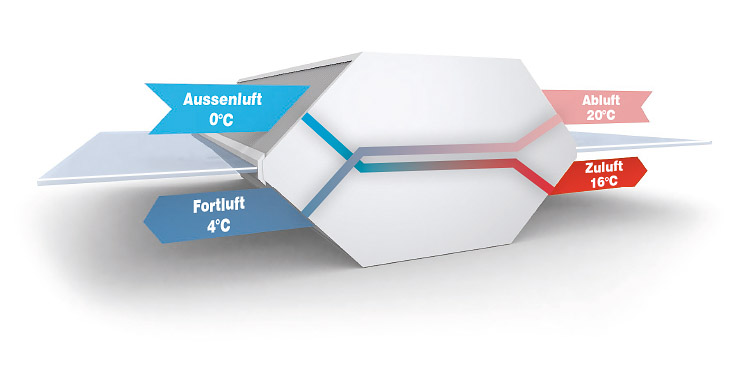
\includegraphics[width=0.7\linewidth]{Bilder/rueckwaermzahl_waermetauscher}
	\caption{Wärmetauscher mit unterschiedlichen Temperaturen (Quelle: \url{http://www.klingenburg.de/fileadmin/user_upload/germany/Wissen/rueckwaermzahlt_de_02.jpg})}
	\label{fig:waermetauscher_wrg}
\end{figure}
 
Die Umsetzung ist im folgenden Code zu sehen. Es werden die drei Temperaturwerte aus den jeweiligen Registern ausgelesen. Daraufhin wird der Wärmerückgewinnungsgrad berechnet, das Ergebnis gerundet und mit der Maßeinheit \enquote{\%} zurückgegeben.

\begin{pythoncode}
def calc_wrg(sensors, additional_info):
	exhaust_air = sensors[0].get_data_from_modbus()  # Abluft
	outgoing_air = sensors[1].get_data_from_modbus()  # Fortluft
	outside_air = sensors[2].get_data_from_modbus()  # Außenluft
	
	wrg = ((exhaust_air - outgoing_air) / (exhaust_air - outside_air)) * 100
	
	return str(round(wrg)) + " %"
\end{pythoncode}

Eine Angabe in der Haupt-Konfigurationsdatei sieht wie folgt aus. Dabei ist zu beachten, dass im \enquote{port} Array zuerst die Quelle der Ablufttemperatur, als zweites die Quelle der Fortlufttemperatur und zuletzt die Quelle der Außenlufttemperatur einer \acs{rltanlage} angegeben werden. Es wird keine \enquote{additional\_info} angegeben.

\begin{jsoncode}
	"sources": [
	{
		"port": [
			{"QBM2": "AI1"},
			{"QBM1": "AI2"},
			{"QBM1": "AI1"}
		],
		"description": "Wärmerückgewinnungsgrad",
		"python_function": "calc_wrg"
	},
	...
	]
\end{jsoncode}



\paragraph{Funktion \enquote{calc\_volume}}
Wird verwendet, um bei ebm-papst Ventilatoren den Volumenstrom zu ermitteln. Dieser gibt an, wie viel Luftvolumen der Ventilator pro Stunde befördert. Zur Bestimmung des Volumenstroms ($q_{V}$) kommt bei ebm-papst das Wirkdruckverfahren zum Einsatz, welches den statischen Druck vor und in der Einströmdüse vergleicht ($\rightarrow$ Differenzdruck der statischen Drücke $\Delta p$). \\
Die Formel für die Berechnung des Volumenstroms \eqref{glg:volumenstrom_berechnung} ist folgend zu sehen, wobei der K-Faktor \bzw Durchflussfaktor \cite[vgl.][]{rox_klimatechnik:o.J.} von der Größe der Einströmdüse abhängt und aus Datenblättern entnommen wird. \cite[vgl.][171]{ebmpapst:2021}

\begin{equation}
	q_{V}\left[\frac{m^{3}}{h}\right] = \text{K-Faktor} \cdot \sqrt{\Delta p} \left[Pa\right]
	\label{glg:volumenstrom_berechnung}
\end{equation} 

Im unten stehenden Code ist die Anwendung der obigen Formel zu sehen. Der Differenzdruck wird dabei aus einem Modbus Register ausgelesen. In manchen Fällen kann es dazu kommen, dass ein Ventilator nicht dreht. Trotzdem ermittelt der Luftdrucksensor eine kleine Druckdifferenz, welche zu unrealistischen Ergebnissen führt. Daher wird unter einer bestimmten Druckdifferenz ein Volumenstrom von 0 zurückgegeben.

\begin{pythoncode}
def calc_volume(sensors, additional_info):
	sensor_value = sensors[0].get_data_from_modbus()
	
	if sensor_value <= 5:
		return_str = "0 m³/h"
	else:
		return_str = str(round(math.sqrt(sensor_value) * additional_info["k-faktor"])) + " m³/h"
	
	return return_str
\end{pythoncode}

Eine Angabe in der Haupt-Konfigurationsdatei sieht wie folgt aus. Dabei ist zu sehen, dass im \enquote{port} Array die Quelle eines Luftdrucksensors angegeben wird. Der K-Faktor wird als \enquote{additional\_info} angeführt.

\begin{jsoncode}
"sources": [
	{
		"port": [
			{"QBM2": "P1"}
		],
		"description": "ZUL. Volumen",
		"python_function": "calc_volume",
		"additional_info": {"k-faktor": 116}
	},
	...
]
\end{jsoncode}



\paragraph{Funktion \enquote{flap\_position}}
Wird verwendet, um die Klappenposition \bzw den Öffnungsgrad einer Klappe zu ermitteln. 
Dazu wird ein Register ausgelesen, das einen Wert zwischen 0 und 10500 $mV$ enthält \cite[vgl.][17]{siemens:2021}, wie im folgenden Code ersichtlich ist. Anschließend wird das Verhältnis des ausgelesenen Werts zum maximalen Wert von 10500 $mV$ berechnet. Das Ergebnis wird gerundet und in Prozent zurückgegeben.

\begin{pythoncode}
def flap_position(sensors, additional_info):
	flap_mv = sensors[0].get_data_from_modbus()
	flap_pos = flap_mv / 10500 * 100
	return str(round(flap_pos)) + " %"
\end{pythoncode}

Eine Angabe in der Haupt-Konfigurationsdatei sieht wie folgt aus. Im \enquote{port} Array wird die Quelle eines Analog Outputs (AO) eines Siemens QBMs angegeben, an das eine Klappe angeschlossen ist. Es wird keine \enquote{additional\_info} angeführt.

\begin{jsoncode}
"sources": [
	{
		"port": [
			{"QBM1": "AO1"}
		],
		"description": "AUL. Klappe",
		"python_function": "flap_position"
	},
	...
]
\end{jsoncode}



\paragraph{Funktion \enquote{relay\_position}}
Wird verwendet, um die Relaisposition \bzw, ob ein Relais offen oder geschlossen ist, zu ermitteln. Dazu wird ein Register ausgelesen, das einen Wert zwischen 0 und 10500 $mV$ enthält \cite[vgl.][17]{siemens:2021}, wie im folgenden Code ersichtlich ist. Anschließend wird überprüft, ob der ausgelesene Werts größer oder kleiner als die angegebene Schaltschwelle ist. Daraus wird der Zustand des Relais abgeleitet.

\begin{pythoncode}
def relay_position(sensors, additional_info):
	relay_mv = sensors[0].get_data_from_modbus()
	if relay_mv < (additional_info["switching_voltage"] * 1000):
		return "Geschlossen"
	else:
		return "Offen"

\end{pythoncode}

Eine Angabe in der Haupt-Konfigurationsdatei sieht wie folgt aus. Im \enquote{port} Array wird die Quelle eines Analog Outputs (AO) eines Siemens QBMs spezifiziert, an das ein Relais angeschlossen ist. Die Schaltschwelle, also die Spannung, bei der das Relais umschaltet, wird als \enquote{additional\_info} in Volt angegeben.

\begin{jsoncode}
"sources": [
	{
		"port": [
			{"QBM1": "AO2"}
		],
		"description": "WRG. Relais",
		"python_function": "relay_position",
		"additional_info": {"switching_voltage": 8}
	},
	...
]
\end{jsoncode}

\section{Auslesen der \acs{rlt} Parameter}
\setAuthor{\schneider}
\label{auslesen_rlt_parameter}

Um über die \gls{gls_rs485} Schnittstelle mit \gls{gls_minimalmodbus} Daten auszulesen wird ein separater \gls{gls_thread} erstellt. In diesem wird die \lstinline{data_refresh()} Funktion ausgeführt. Diese Funktion kann nicht im Hauptthread laufen, da \gls{gls_ctk} den Hauptthread blockiert. Außerdem wird durch den Einsatz von \gls{gls_thread}s die Last besser verteilt. Beim Erstellen des \gls{gls_thread}s wird angegeben, dass die \lstinline{data_refresh()} Funktion darin ausgeführt wird. Als Parameter erhält diese die \gls{gls_ctk} \lstinline{app} Instanz (siehe Kapitel \ref{tkintercode}). Außerdem deklariert man ihn als \gls{gls_daemon} \gls{gls_thread}. Dadurch kann das Programm terminieren, auch wenn der \gls{gls_daemon} \gls{gls_thread} noch nicht geendet hat.

\begin{pythoncode}
def data_threading(app):
	t1 = Thread(target=data_refresh, kwargs={'app': app}, daemon=True)
	t1.start()
\end{pythoncode}

In diesem \gls{gls_thread} werden periodisch, jeweils in 0,4 Sekunden Abständen die Daten der Sensoren erneuert. Die Sensoren sind in den Measurements gespeichert. Es werden alle \lstinline{Page} Instanzen und darin alle \lstinline{Measurement} Instanzen iteriert und die \lstinline{run_calculation()} Methode aufgerufen. Diese liefert den ausgelesenen Wert zurück, der dann auf der \acs{gui} an der entsprechenden Stelle umgeändert wird. Dies passiert mit der \lstinline{set_page_text_at()} Methode der \lstinline{App} Klasse (siehe Kapitel \ref{tkintercode}). 
\newline Mit dieser Implementierung werden kontinuierlich alle Werte ausgelesen und erneuert. Dadurch können beim Wechseln der Seite sofort die zuletzt verfügbaren Messwerte angesehen werden. Würde immer nur die aktuelle Seite geladen werden, wäre das Programm zwar etwas effizienter, aber beim Umschalten der Seite zeigen die Messwerte überall "N/A"\ bzw. veraltete Werte an, bis die Daten erneuert werden. 

\begin{pythoncode}
def data_refresh(app):
	while True:
		page_counter = 0
		for page in all_pages:
			measurement_counter = 0
			for measurement in page.measurements:
				value = measurement.run_calculation()
				app.set_page_text_at(page_counter, measurement_counter, measurement.description, value)
				measurement_counter += 1
			page_counter += 1
		
		time.sleep(0.4)
\end{pythoncode}

Die \lstinline{Sensor} Instanzen lesen dann mithilfe von \gls{gls_minimalmodbus} die Register der am Bus angeschlossenen Geräte aus. Im Konstruktor der \lstinline{Sensor} Instanzen wird die Kommunikation aufgesetzt. Es gibt eine Vielzahl von Parametern, die aus den Konfigurationsdateien ausgelesen werden, welche hier beschrieben werden (vgl. Kapitel \ref{json_config_files}). Damit wird eine \lstinline{Instrument} Instanz erstellt, welche mit den Parametern konfiguriert wird. Zuletzt werden noch zwei Optionen auf \enquote{True} gesetzt. Zum Einen wird \lstinline{clear_buffers_before_each_transaction()} aktiviert. Dadurch werden Lese- und Schreibpuffer nach jedem Zugriff geleert. Dies verhindert das Auftreten mancher Fehler. Außerdem wird \lstinline{close_port_after_each_call()} aktiviert, damit der Port nach jedem Zugriff geschlossen wird. Wenn das Programm terminiert, wird der \gls{gls_thread} auch terminiert. Wenn der Port nun nach jedem Zugriff geschlossen wird, werden somit weitere Fehler verhindert.

\begin{pythoncode}
class Sensor():
	def __init__(self, baud_rate, mb_address, parity, stop_bits, scaling, register, function_code, zero_based):
		self.sensor = minmb.Instrument('/dev/ttyAMA0', mb_address)
		self.sensor.serial.baudrate = baud_rate
		self.sensor.serial.bytesize = 8
		
		if parity == "even":  # ODD, EVEN oder NONE
			self.sensor.serial.parity = minmb.serial.PARITY_EVEN
		elif parity == "odd":
			self.sensor.serial.parity = minmb.serial.PARITY_ODD
		else:
			self.sensor.serial.parity = minmb.serial.PARITY_NONE
		
		self.sensor.serial.stopbits = stop_bits
		self.sensor.serial.timeout = 0.5
		self.sensor.mode = minmb.MODE_RTU
		
		self.sensor.clear_buffers_before_each_transaction = True
		self.sensor.close_port_after_each_call = True
\end{pythoncode}

Beim Erstellen der \lstinline{Instrument} Instanz wird als erster Parameter angegeben, an welchem Port am Raspberry PI der Adapter angeschlossen ist bzw. über welchen Port die Kommunikation stattfindet. Dabei muss je nach Plattform und Adapterart ein anderer Gerätestring angegeben werden:
\begin{itemize}
\item \textbf{COMn:} Damit kann auf Windows die Kommunikation mit \gls{modbus} über einen USB Connector aufgesetzt werden. Die Nummer n am Ende der Zeichenkette, ist dabei bei jedem PC / Port unterschiedlich und wird intern vergeben. Man muss diese vorher im Gerätemanager nachschauen und kann dann die entsprechende Nummer verwenden. Hier fand es seinen Einsatz insbesondere bei den anfänglichen Ausleseversuchen und den ersten Programmversionen.
\item \textbf{/dev/ttyUSB0:} Damit kann auf Linux die Kommunikation mit \gls{modbus} über einen USB Connector aufgesetzt werden. Benutzt wurde dieses beim Testen des Programms auf dem Raspberry PI, als der erste \gls{gls_rs485} Adapter noch nicht geliefert war bzw. nicht funktionierte.
\item \textbf{/dev/ttyAMA0:} Damit kann auf Linux über die \ac{uart} Pins, also genauer gesagt Pin 8 (TX) und Pin 10 (RX) kommuniziert werden. Im finalen Programm wird das verwendet, da dieses auf dem Raspberry PI läuft und über die \ac{uart} Pins kommuniziert. Die Pins sind dabei über einen funktionierenden \gls{gls_rs485} Adapter als Zwischenstück an dem Bussystem angeschlossen.
\end{itemize}

\vfill

\label{get_data_from_modbus}
In der \lstinline{get_data_from_modbus()} Methode, welche auch Teil der \lstinline{Sensor} Klasse ist, wird dann das entsprechende Register mithilfe der von \gls{gls_minimalmodbus} bereitgestellten \lstinline{read_registers()} Funktion ausgelesen. In der Parameterliste gibt man die Registernummer, die Anzahl an auszulesender Register und den \gls{modbus} Function Code an. Der ausgelesene Wert wird dann entsprechend der in der Konfigurationsdatei angegebenen Skalierung angepasst und zurückgeliefert. Diese Methode wird innerhalb der konfigurierbaren Funktionen der \enquote{modbus\_functions.py} Datei aufgerufen (vgl. Kapitel \ref{python_functions}).

\begin{pythoncode}
class Sensor():
	def get_data_from_modbus(self):
		try:
			fetched_data = self.sensor.read_registers(self.register, 1, self.function_code)
			fetched_data_scaled = round((fetched_data[0] * self.scaling), 1)
			return fetched_data_scaled
		
		except Exception as e:
			print("Err: ", str(e))
			return "N/A"
\end{pythoncode}

In der \lstinline{run_calculation()} Methode der \lstinline{Measurement} Instanz wird die in der Konfigurationsdatei angegebene Funktion ausgewählt. Wenn \enquote{standard} eingelesen wurde, wird die Standard Funktion ausgeführt. Ansonsten wird mit \lstinline{hasattr()} überprüft, ob innerhalb der \enquote{modbus\_functions} Datei die angegebene Funktion existiert. Wenn diese existiert, wird mit \lstinline{getattr()} ein Funktionszeiger erstellt. Mit diesem Zeiger wird dann die entsprechende Funktion ausgeführt. Welche Funktionen vorhanden sind wird in Kapitel \ref{python_functions} beschrieben. 

\begin{pythoncode}
class Measurement():
	def run_calculation(self):
		try:
			if self.python_function == "standard":
				self.value = str(modbus_functions.standard(self.sensors, self.additional_info)) + " " + self.unit
			elif (hasattr(modbus_functions, self.python_function)):
				calc_function = getattr(modbus_functions, self.python_function)
				self.value = str(calc_function(self.sensors, self.additional_info))
			else:
				self.value = "python function was invalid"
		
			return self.value
		except Exception as e:
			print("Err: ", e)
\end{pythoncode}

\section{Fertigstellung}
\setAuthor{\schneider}
\subsection{Übertragen der Config Files mittels USB}
Um dem Programm die neuesten Konfigurationsdateien zu übergeben, steckt man beim Bootvorgang des Raspberry Pi einen Datenträger (\zB USB-Stick) an. Auf dem Datenträger muss im Root-Verzeichnis (\textasciitilde) ein Verzeichnis namens "'RLT\_Config"' sein. Wenn dieses Verzeichnis und alle nötigen Konfigurationsdateien darin vorhanden sind, werden diese in das Documents-Verzeichnis des Raspberry Pi kopiert. Das passiert in der "'usb\_routine"' Funktion. Diese Funktion liefert einen Fehlercode zurück, der daraufhin in einer Verzweigung abgefragt wird. Wenn ein Fehler beim Übertragen auftritt, terminiert das Programm. Ansonsten fährt das Programm fort.

In DIA ein Ablaufdiagramm erstellen.
Folgendes Diagramm verdeutlicht diesen Vorgang. Es wurde mit einem Programm namens Dia erstellt.

%\pythonfile[firstline=2, lastline=12]{Code/main.py}

\begin{pythoncode}
if __name__ == "__main__":
	copy_error = usb_detection.usb_routine()
	if copy_error:
		exit
	all_pages = modbus.load_config()
	global app
	app = App(all_pages)
	setup_buttons()
	modbus.data_threading(app)
	app.mainloop()	
\end{pythoncode}

Es wird die "copy\_from\_usb"\ Funktion aufgerufen. Diese gibt einen Statuscode zurück. Die \dq start\_window"\ Funktion erstellt ein neues customtkinter Fenster, in dem dann der Parameter string angezeigt wird. Das Fenster bleibt für sieben Sekunden offen, bevor es wieder geschlossen wird und die Ausführung fortfährt.

\begin{pythoncode}
def usb_routine():
	copy_error = copy_from_usb()
	if copy_error == -1:
		return True
	elif copy_error == 0:
		start_window("Config Dateien wurden kopiert. Entferne nun den USB")   
	elif copy_error == 1: 
		start_window("Kein USB-Stick gefunden und Config bereits vorhanden")  
	return False
\end{pythoncode}

Es folgt die Beschreibung der "copy\_from\_usb"\ Funktion. Es wird geschaut ob auf einem der sd-Ports ein Datenträger angeschlossen ist. Wenn ja, wird der entsprechende Port gespeichert und die Abfrage beendet. Wenn kein Datenträger gefunden wird, kann man davon ausgehen, dass keine Änderung an der Konfiguration vorgenommen werden soll. Es wird nun überprüft, ob im Programmverzeichnis alle benötigten Konfigurationsdateien vorhanden sind. Das passiert im "check\_if\_files\_exists". Wenn ja, ist der Kopiervorgang abgeschlossen, wenn nein, wird der Vorgang wiederholt, bis ein Datenträger gefunden wird. Die Ausführung wird für fünf Sekunden gestoppt, damit der Benutzer oder die Benutzerin genügend Zeit hat einen Datenträger einzufügen.

\begin{pythoncode}
	port = ""
	while True:
		if (os.system("mount | grep sda1") != 256):
			port = "sda1"
			break
		elif (os.system("mount | grep sdb1") != 256):
			port = "sdb1"
			break
		elif (os.system("mount | grep sdc1") != 256):
			port = "sdc1"
			break
		elif (os.system("mount | grep sdd1") != 256):
			port = "sdd1"
			break
		
		if (check_if_files_exists(config_path, device_config_path, False)):
			return 1
			
		time.sleep(5)
\end{pythoncode}

Wenn ein Datenträger gefunden wurde, wird dieser Port gemountet. Dieses mal wird überprüft, ob die Konfigurationsdateien auf dem Datenträger existieren. Wenn nicht, wird der Datenträger ausgeworfen und ein Fehlercode zurückgegeben. Ansonsten werden die Dateien kopiert und der Datenträger ausgeworfen. Die beiden Funktionen "check\_if\_files\_exists"\ und \dq start\_window"\ sind im Codeanhang zu finden. Beim Auswerfen wird manchmal eine Nachricht angezeigt, dass der Datenträger nicht ausgeworfen wurde. Dies kann ignoriert werden (Quelle angeben; falls das überhaupt stimmt).

\begin{pythoncode}
	os.system("sudo umount /dev/" + port)
	os.system("sudo mount /dev/" + port + " /home/pi/Documents/Config")
	
	error_free = check_if_files_exists(usb_config_path, usb_device_config_path, True)
	if error_free:
		os.system("cp -r ~/Documents/Config/RLT_Config ~/Documents/")
	else:
		os.system("sudo umount /dev/" + port)
		#os.system("sudo eject /dev/" + port) 
		#os.system("udisk --detach /dev/" + port)
		return -1
		
	os.system("sudo umount /dev/" + port)
	#os.system("sudo eject /dev/" + port) 
	#os.system("udisk --detach /dev/" + port)
	return 0
\end{pythoncode}

\setAuthor{\pezze}
 \subsection{Der Prototyp}
Der Prototyp der \ac{rltanzeige} ist funktionsfähig in Abb.~\ref{fig:tdot_anzeige} (siehe Kapitel \ref{rltanzeige_tdot_kapitel}) zu sehen. In diesem Abschnitt wird kurz der Aufbau dieses Prototyps (siehe Abb.~\ref{fig:rlt_anzeige_prototyp}) erklärt. 

\begin{figure}[H]
    \begin{subfigure}[l]{0.48\textwidth}
        \centering
        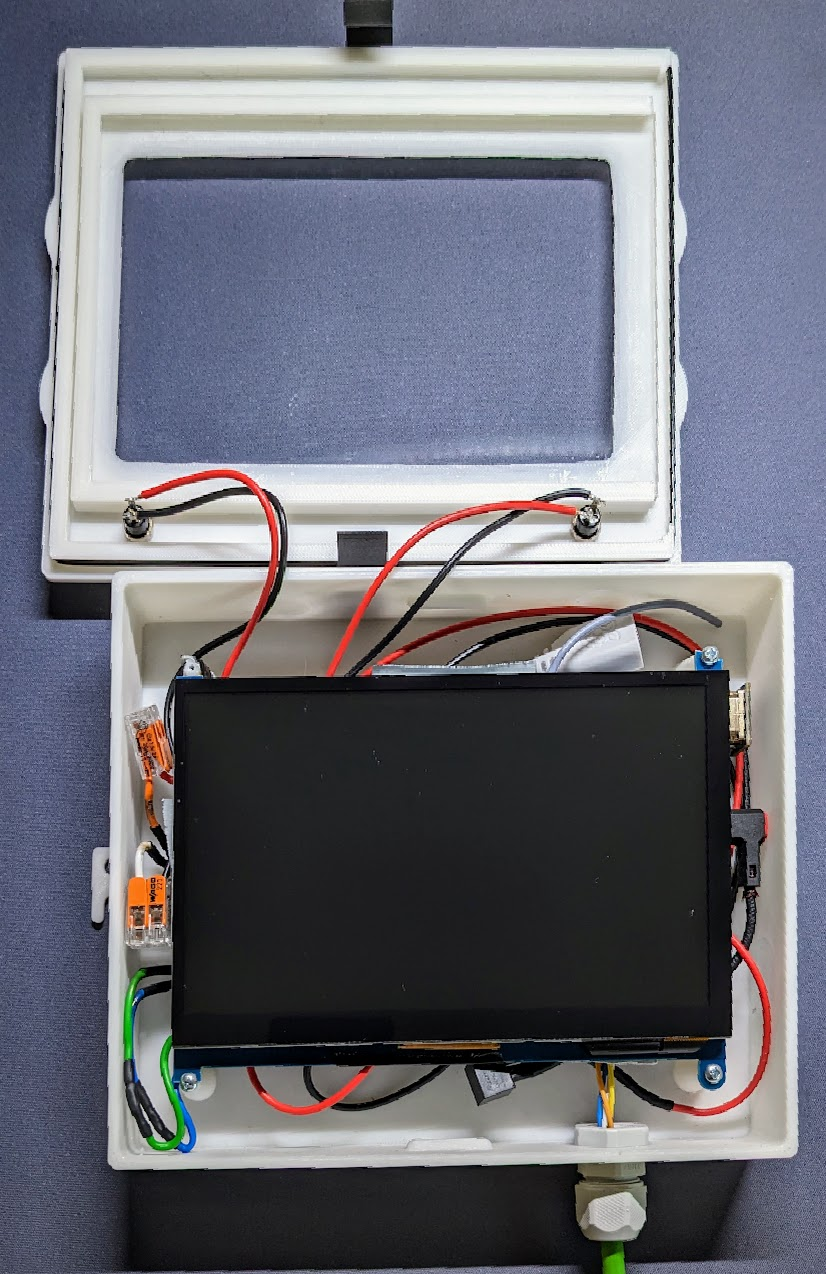
\includegraphics[width=0.99\textwidth]{prototyp_offen_w_display}
        \caption{Prototyp mit eingebautem Display \label{fig:prototyp_w_display}}
    \end{subfigure}
    \hfill
    \begin{subfigure}[r]{0.504\textwidth}
        \centering
        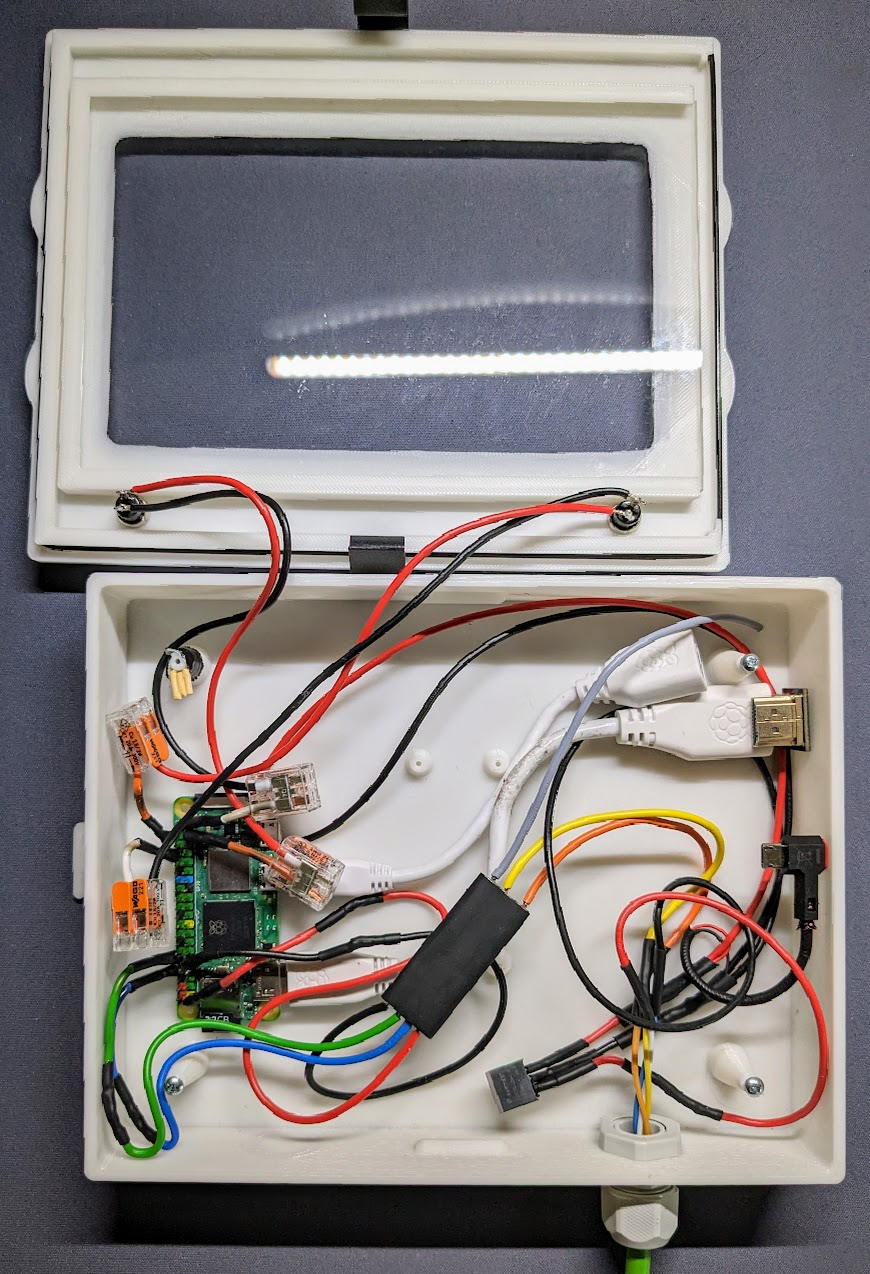
\includegraphics[width=0.99\textwidth]{prototyp_offen_w_o_display}
        \caption{Prototyp mit ausgebautem Display \label{fig:prototyp_w_o_display}}
    \end{subfigure}
	\caption{Prototyp der \ac{rltanzeige} von innen \label{fig:rlt_anzeige_prototyp}}
\end{figure}

Das Gehäuse des Prototyps ist 3D-gedruckt, um schnell Anpassungen machen zu können und nicht von einem vorgefertigten Gehäuse eingeschränkt zu werden. In diesem Gehäuse sind folgende Komponenten verbaut:

\begin{itemize}
    \item Der \textbf{Raspberry PI Zero 2 W} (siehe Abb.~\ref{fig:zero_2_w}) dient aufgrund seiner kleinen Größe und Rechenleistung als Rechner. Die Unterstützung von WLAN und Bluetooth lässt außerdem Raum zur Weiterentwicklung der \ac{rltanzeige}.
    \begin{figure}[H]
        \centering
        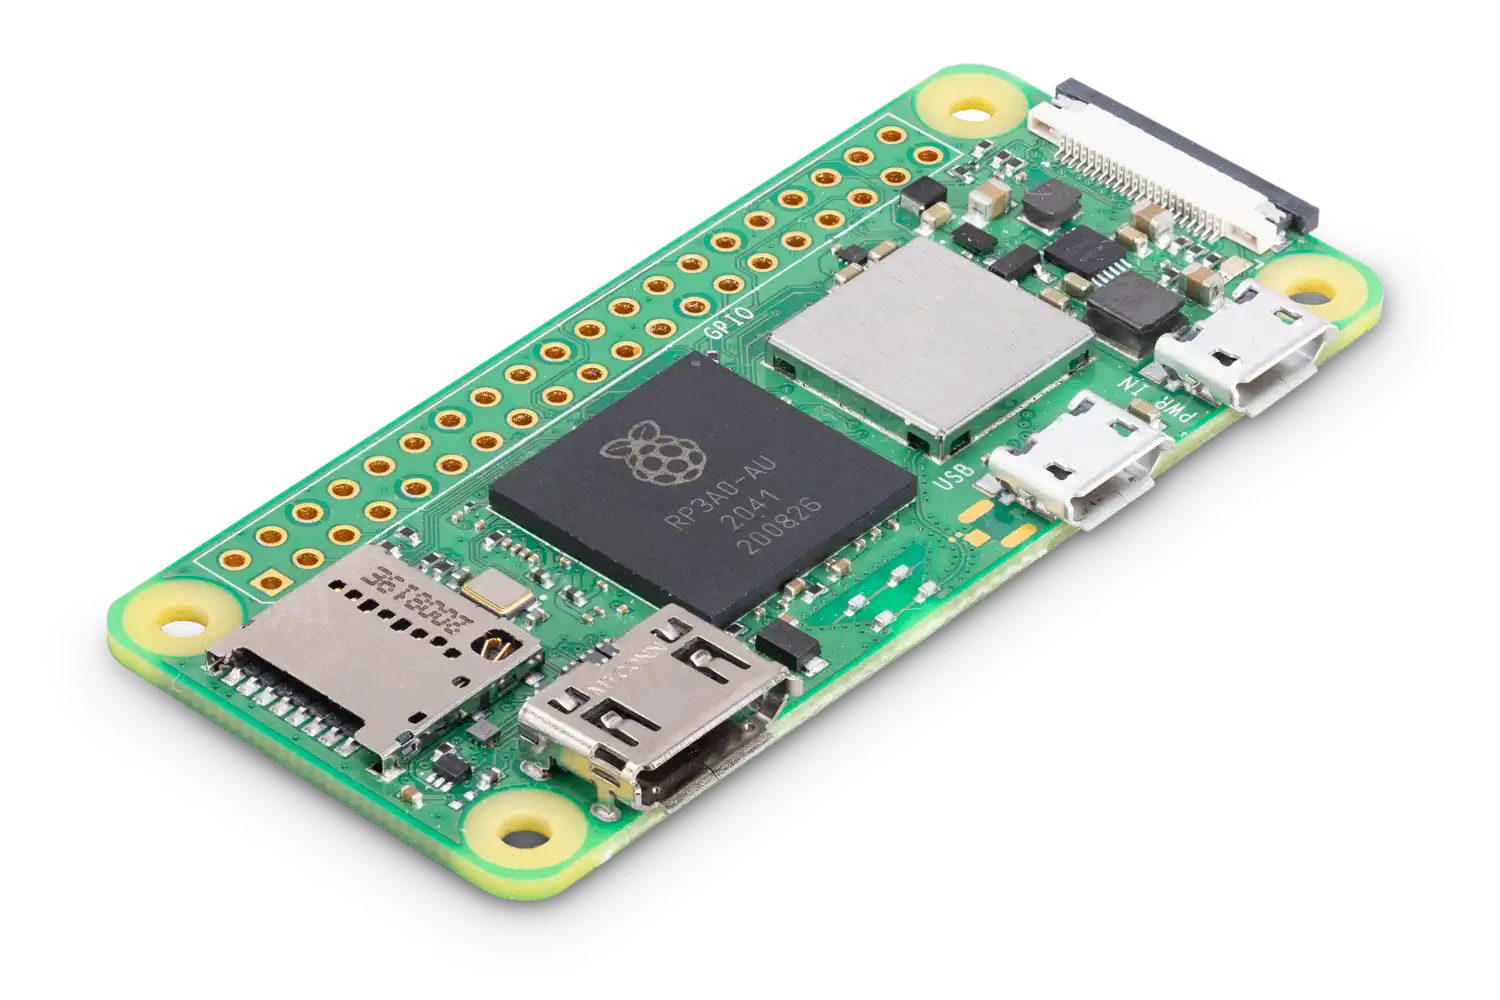
\includegraphics[width=7cm]{zero2-hero}
        \caption{Raspberry PI Zero 2 W (Quelle: \url{https://www.raspberrypi.com/products/raspberry-pi-zero-2-w/}) \label{fig:zero_2_w}}
    \end{figure}
    
    \item Das \textbf{7-Zoll Display} wird über \ac{hdmi} mit dem Raspberry PI verbunden und über Micro-USB mit Strom versorgt.

    \item Der \textbf{\ac{uart} zu \gls{gls_rs485} Adapter} (siehe Abb.~\ref{fig:ttl_rs485_adapter}) dient als Zwischenstück zwischen dem Raspberry PI und dem Bussystem. So kann das \gls{gls_rs485} Kabel mit den \ac{uart} Pins des Raspberry PIs verbunden werden.
    \begin{figure}[H]
        \centering
        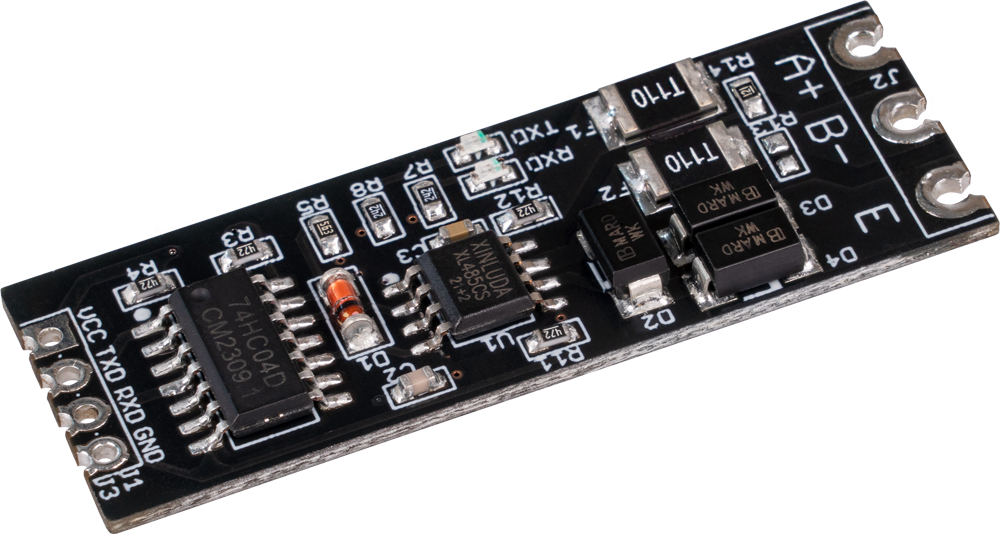
\includegraphics[width=6cm]{COM-TTL-RS4851}
        \caption{Joy-IT \ac{uart} TTL - \gls{gls_rs485} Konverter (Quelle: \url{https://joy-it.net/de/products/COM-TTL-RS485}) \label{fig:ttl_rs485_adapter}}
    \end{figure}

    \item Der \textbf{Spannungswandler} (siehe Abb.~\ref{fig:spannungswandler}) \bzw DC/DC Wandler wird benötigt, um die eingehende Spannung von 24 V auf 5 V zu reduzieren. Dabei werden sowohl der Raspberry PI als auch das Display von dieser Stromquelle versorgt.
    \begin{figure}[H]
        \centering
        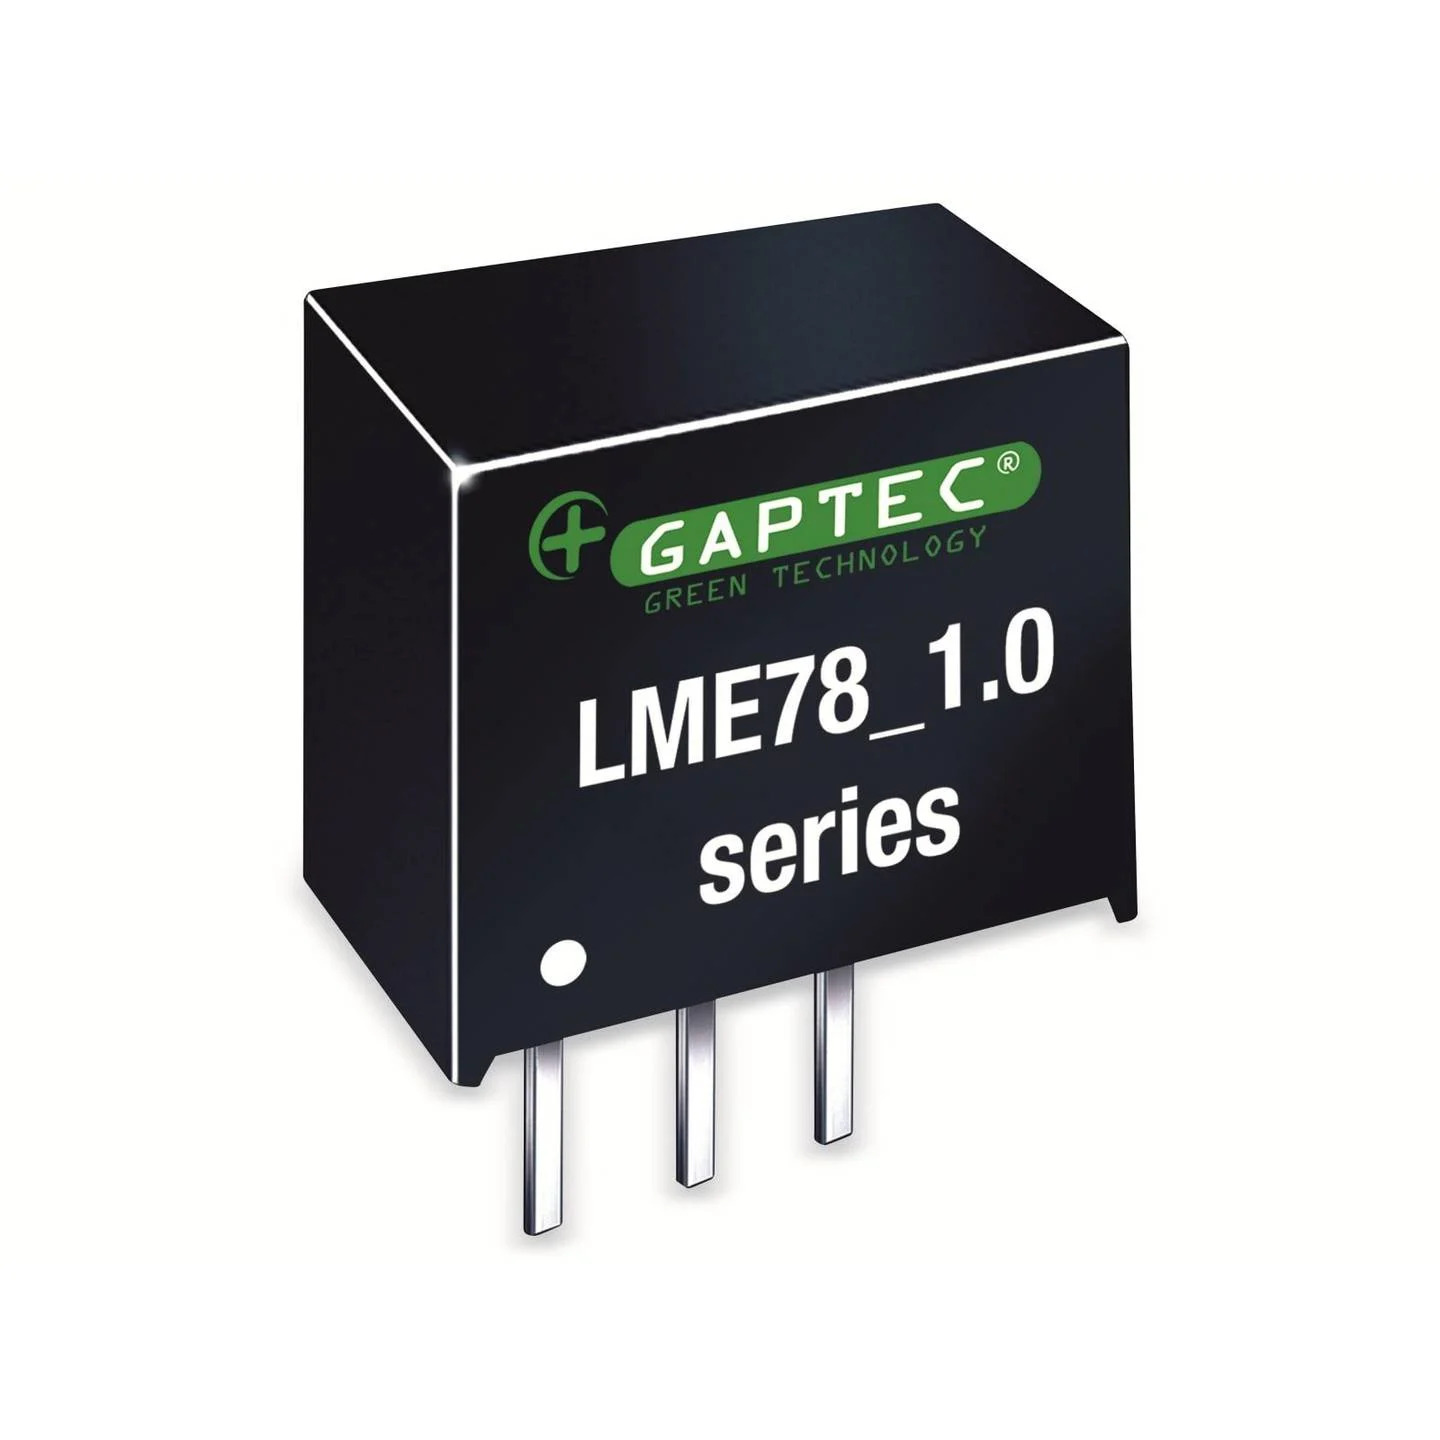
\includegraphics[width=5cm]{spannungswandler}
        \caption{Gaptec LME78\_05-1.0 DC/DC Wandler (Quelle: \url{https://www.conrad.de/de/p/gaptec-dc-dc-wandler-electronic-sip3-8-36vin-5vout-1000ma-11-6x8x10-4mm-856967933.html}) \label{fig:spannungswandler}}
    \end{figure}
\end{itemize}
\subsection{Erstellung des Raspberry PI \textit{Images}}
Technikerinnen und Techniker müssen die Schritte zum Aufsetzen eines Raspberry PIs (siehe Kapitel \ref{raspi_setup}) bei einer Neuinstallation nicht durchführen, da ihnen ein vorgefertigtes \gls{image} verabreicht wird. Dieses muss lediglich auf die SD-Karte des Raspberry PIs kopiert und nicht weiter konfiguriert werden. Die Erstellung dieses \gls{image}\textit{s} wird folgend erläutert. Das \gls{image} wird über ein Gerät mit Linux erstellt, daher kommt eine \ac{vm} zum Einsatz, um einfach eine Linux Distribution auf einem Windows Gerät laufen zu lassen. Dabei können unterschiedliche Linux Distributionen verwendet werden, wobei mindestens $4$ Gigabyte Arbeitsspeicher, $2$ Prozessorkerne und $80$ Gigabyte Festplattenspeicher empfohlen werden. 

\paragraph{\textit{Image} klonen}
Das \gls{image} wird erstellt, indem ein Speicherabbild einer SD-Karte mit funktionierendem Betriebssystem und Python Programm gemacht wird. Dieser Prozess findet hauptsächlich in der Kommandozeile statt, daher muss das Linux-Terminal geöffnet werden, um die folgenden Befehle auszuführen:
\begin{enumerate}
    %\item Zur Vorbereitung wird GParted mit \mintinline{console}{sudo apt-get install gparted} installiert. 

    \item Um die SD-Karte zu klonen, muss zuerst ihr Pfad mithilfe des Befehls \mintinline{console}{sudo fdisk -l} ermittelt werden. Dabei ist in Abb. \ref{fig:sudo_fdisk} zu sehen, dass der Pfad in diesem Beispiel \enquote{dev/sdb} ist.
    \begin{figure}[H]
        \centering
        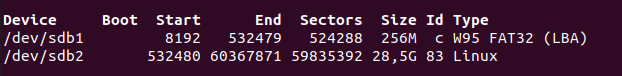
\includegraphics[width=0.75\linewidth]{sudo_fdisk}
        \caption{Ergebnis des \mintinline{console}{sudo fdisk -l} Befehls im Linux Terminal}
        \label{fig:sudo_fdisk}
    \end{figure}
    
    \item Im nächsten Schritt kann die SD-Karte geklont werden. Dazu wird der Befehl \mintinline{console}{dd} verwendet, wobei bei \mintinline{console}{if=} das input file \bzw der Pfad der SD-Karte angegeben wird und bei \mintinline{console}{of=} das output file \bzw der Pfad der \gls{image} (\enquote{.img}) Datei angegeben wird:
    \begin{minted}{console}
sudo dd if=/dev/sdb of=/home/ubuntu/Desktop/clone.img
    \end{minted}

    \item Da die aus dem vorgehenden Befehl generierte \gls{image} Datei mehr als $30$ Gigabyte groß ist, kann das \enquote{PyShrink} Skript verwendet werden, um das große  \gls{image} auf etwa $5$ bis $6$ Gigabyte zu verkleinern. \enquote{PyShrink} wird mit den folgenden Befehlen über die Kommandozeile installiert:
    \begin{minted}[breaklines=true, breakanywhere=true]{console}
wget https://raw.githubusercontent.com/Drewsif/PiShrink/master/pishrink.sh
chmod +x pishrink.sh
sudo mv pishrink.sh /usr/local/bin
    \end{minted}

    Nach der Installation, kann das \gls{image} mithilfe des nachfolgenden Befehls verkleinert werden. Hier wird ebenfalls zuerst der Pfad der Eingabedatei und dann der Pfad der Ausgabedatei angegeben:
    \begin{minted}[breaklines=true, breakanywhere=true]{console}
sudo pishrink.sh /home/ubuntu/Desktop/clone.img /home/ubuntu/Desktop/shrunken-image.img
    \end{minted}

    \item Das verkleinerte Image kann nun auf eine neue SD-Karte geflasht werden. Dafür kann ein beliebiger Imager, wie \zB \enquote{balenaEtcher} \enquote{Win32DiskImager} oder \enquote{RaspberryPi-Imager}, genutzt werden.
\end{enumerate}





\newpage
\section{aufgetretene Problematiken}
\setAuthor{\mangeng}
Eine Normalität während der Ausarbeitung eines Projektes sind auftretende Probleme. Während kleinere den Arbeitsfluss nicht stören, können größere wiederum Einbußen in den Zeitplänen bedeuten. Nichtsdestotrotz stärken sie im Allgemeinen das Teamwork und man entwickelt sich auf persönlicher Ebene.\\ Folgend sind die größten Probleme festgehalten, die während dieser Diplomarbeit auftraten.

\begin{enumerate}
	\item \textbf{Hardware:} Nachdem die Hardwareevaluierung abgeschlossen und die Entscheidung dem Projektbetreuer Simon Köldorfer mitgeteilt worden war, wurde eine Anzahl an Raspberry Pis, SD-Cards und ein Display zur Verfügung gestellt, um bereits während des Wartens auf die eigentlichen Komponenten mit teilweise erhöhten Lieferzeiten bereits arbeiten zu können. Relativ schnell wurde festgestellt, dass auf der einen SD-Card nur eine veraltete Version von Python installierbar war und auf der anderen die Python-Version zwar auf die derzeit neueste aktualisiert werden konnte, aber das Display aus unbekannten Gründen nicht damit kompatibel war. Da nun die SD-Card mit der veralteten Version ausgeschlossen wurde, musste eine Lösung für die andere gefunden werden. Mit der Applikation \enquote{Real VNC Viewer} konnte, ohne Verwendung des Displays, auf den Raspberry Pi zugegriffen werden. So wurde mit dem Programm als Anzeigelösung gearbeitet, bis das eigentlich gewünschte Display die Firma erreicht und auch funktionierende SD-Cards zur Verfügung standen. Nach wenigen Tagen wurde dann ein weiteres Problem bemerkt, denn der Raspberry Pi konnte übergangslos keine WLAN-Verbindung mehr herstellen. Dies zwang dazu, auf eine außergewöhnliche Methode umzusteigen, damit der Zugriff auf den Raspberry Pi gewährt werden konnte. Durch die Verwendung mehrerer Ethernetkabel, die mit dem Mikrocontroller, den Laptops und einem Switch verbunden wurden, konnte der Zugriff mittels des Programmes \enquote{PuTTy} gewährt werden.
	\item \textbf{Lieferung der Komponenten:} Bevor die gewünschte und erwartete Hardware in der Firma eintraf, wurde der Code bereits passend für das eigentlich bestellte Display geschrieben. Aufgrund von Komplikationen konnte besagtes Gerät nicht beschaffen werden, was dazu führte, dass der Code vollständig überarbeitet werden musste. Zudem wurde das neue Display über \gls{hdmi} an den Raspberry Pi angeschlossen und nicht über \gls{gpio}, wie es bei dem gewünschten Display gewesen wäre. Diese unerwarteten Veränderungen haben die Entwicklungszeit verlängert und erforderten zusätzliche Anpassungen.
	\item \textbf{Modbus-Auslesung:} Ein weiteres Problem wurde bei der Auslesung der Modbus-Daten festgestellt. Obwohl das Lesen der Temperatur- und Drucksensoren schnell und akkurat sowohl in \enquote{Shortbus} als auch im Code funktionierte, wurde ein Hindernis bei den Ventilatoren angetroffen, da hier hexadezimale Zahlen bei den Modbusregistern verwendet wurden und somit auch im eben genannten Programm einige Einstellungen geändert werden mussten. Nach langer Suche nach den richtigen Einstellungen konnte nun endlich ein weiterer Erfolg verzeichnet werden. Als dann der Code am Lüftungsgerät ausprobiert wurde, stieß man auf ein weiteres Problem in dieser Thematik. Im Code befand sich fälschlicherweise eine Zeile, die zwar passend für Druck- und Temperatursensoren war, aber nicht für die Ventilatoren. Bevor diese Zeile gefunden worden ist und der Code sowie die Datenauslesung einwandfrei funktionieren konnten, wurde die Suche vergebens nach neuen Modbus-Libraries gestartet.
	\item \textbf{Modbus-Adapter und Gehäuse:} Im Zusammenhang mit der Hardware traten zwei zusätzliche Probleme auf, die den Abschluss des praktischen Teils verzögerten. Aufgrund von Lieferschwierigkeiten mit dem Display wurde eine Alternative beschafft, die jedoch ebenfalls Komplikationen mit sich brachte, da sie seitlich statt unten angeschlossen wurde. Dies führte dazu, dass das zuvor ausgewählte Gehäuse zu klein war. Die Firma Bösch entschied sich, das richtige Gehäuse selbst per 3D-Drucker herzustellen. Zudem gab es eine Herausforderung mit dem RS485-Modbus-Adapter, die erst bei der Rückkehr in die Firma nach Beendigung des Praktikums gelöst werden konnte, indem andere Adapter dieser Art getestet wurden.
	\item \textbf{Kommunikation:} Dadurch, dass das Pflichtenheft nicht direkt von Anfang an sorgfältig bearbeitet und unterschrieben wurde, konnte nicht verhindert werden, dass in internen Meetings weitere Spezifikationen und Anforderungen an das Projekt hinzugefügt wurden, welche zusätzlichen Aufwand und Verzögerungen mit sich brachten. Bezüglich Meetings hätte auch das Design-Meeting viel früher passieren müssen. Denn es wurde erst im späteren Projektverlauf klar, welche Werte tatsächlich auf dem Display angezeigt werden sollten. Beide genannten Punkte hätten vermieden werden könne, wenn die Kommunikation mit dem Projektbetreuer aktiver gewesen wäre.
\end{enumerate}


%Kapitel von Mangeng
\chapter{Projektmanagement}
\setAuthor{\mangeng}

\section{Projektzieleplan}
In einem Projektzieleplan werden erwartete, messbare Ergebnisse beschrieben und zwischen den folgenden Punkten unterteilt:
\begin{itemize}
	\item \textbf{Haupt-Ziele:} An den Haupt-Zielen wird der  Projekterfolg gemessen. Sie umfassen die Ergebnisse der Diplomarbeit.
	\item \textbf{Neben-Ziele:} Neben- \bzw Zusatz-Ziele sind spezifische Ziele, die zusätzlich neben dem Hauptziel verfolgt werden. Sie können die Qualität eines Produktes erhöhen \bzw den Gesamterfolg des Produktes unterstützen.
	\item \textbf{Nicht-Ziele:} Nicht-Ziele dienen der genaueren Eingrenzung, was in einem Projekt erreicht werden soll. Damit werden Aktivitäten und Prozesse klar ausgegrenzt.
\end{itemize}
Die zu erreichenden Ziele werden meist innerhalb eines Meetings im Team ausgemacht. Treten Veränderungen bei diesen auf, durch beispielsweise Komplikationen, müssen diese Änderungen der Ziele dokumentiert werden \cite[vgl.][]{Diplomarbeiten-bbs:o.J.}. \\ 
Die folgende Tabelle \ref{tab:ziele_plan} beschreibt die Haupt-, Neben- und Nicht-Ziele, die für die Umsetzung dieser Diplomarbeit gelten.
\begin{table}[htpb]
	\caption{Zieleplan}
	\label{tab:ziele_plan}
	\begin{tabular}{p{\dimexpr 0.15\textwidth-2\tabcolsep} | p{0.80\textwidth}}
		\toprule
		\textbf{Zielart} & \textbf{Projektziele} \\
		\midrule
		& Visualisierung der Lüftungsgerät-Werte
		\\
		& Soll parametrierbar ausgeführt werden
		\\
		Hauptziele & Software-Schnittstelle (Zugriff mittels RS323 Schnittstelle)
		\\
		& Kosten in wirtschaftlich sinnvollem Raum
		\\
		& Gehäuse IP66 geschützt 
		\\
		\midrule
		& Nur Werte anzeigen, die auch vorhanden sind (Modbus)
		\\
		& Anleitung für User und Techniker erstellen
		\\
		Nebenziele & Die Anzeige wurde als master definiert. Jetzt sollte sie als Slave definiert werden
		\\
		& Soll QR-Code haben, der beim Scannen die Anzeige am Handy anzeigt
		\\
		\midrule
		& Soll eine Steuerungseinheit darstellen
		\\
		Nichtziele & Benutzerverwaltungsmöglichkeit
		\\
		& Bildschirm- und Bediensperre
		\\
		\bottomrule
	\end{tabular}
\end{table}

\newpage
\newpage
\section{Projektumweltanalyse}
Damit in einem Projekt Veränderungen und Entwicklungen in Umwelten frühzeitig erkannt werden können, um richtig reagieren zu können, werden Umweltanalysen angefertigt. Hier werden die Umfelder nach verschiedenen Kriterien analysiert, die das Unternehmen auf eine gewisse Art beeinflussen. Das tatsächliche Ziel ist es, eine Übersicht über die Umwelten zu haben, um Handlungsempfehlungen ausgeben zu können. Im Marketing wird zwischen internen und externen Faktoren unterschieden \cite[vgl.][]{wikipedia:2023, marketing:2024}.

\section{Projektorganigramm}
Ein Projektorganigramm ist ein wichtiges Instrument zur Darstellung der internen Struktur und der wechselseitigen Beziehungen innerhalb eines Projektteams. Es ermöglicht einen klaren Überblick über die verschiedenen Rollen und Verantwortlichkeiten der Mitarbeiter, sowie deren Hierarchieebenen und deren jeweilige Berichtswege \cite[vgl.][]{projektmanagement-definitionen:2009}. \\
Die folgende Abbildung \ref{fig:organigramm} stellt die existierende, interne Struktur der Diplomarbeit dar, welche daraufhin in der Tabelle \ref{tab:projektorganisation} deutlicher beschrieben wird.

\begin{figure}[H]
	\centering
	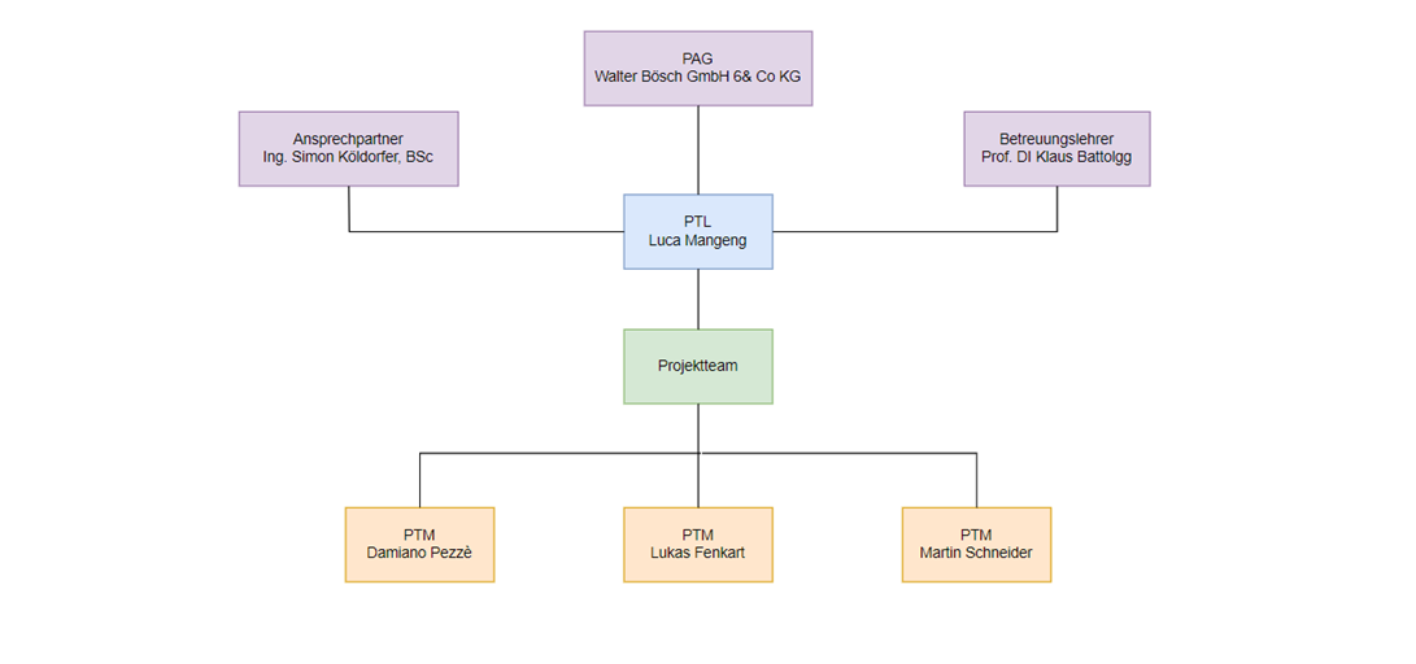
\includegraphics[width=1\linewidth]{Bilder/Organigramm}
	\caption{Projektorganigramm}
	\label{fig:organigramm}
\end{figure}

\begin{table}[H]
	\caption{Projektorganisation}
	\label{tab:projektorganisation}
	\begin{tabular}{p{\dimexpr 0.25\textwidth-2\tabcolsep} | p{0.50\textwidth} | p{0.20\textwidth}}
		\toprule
		\textbf{Projektrolle} & \textbf{Aufgabenbereich/Skills} & \textbf{Name} \\
		\midrule
		Projektauftraggeber & Gibt den Auftrag für die Universalananzeige und setzt Bedingungen und Ziele, die im Projekt erreicht werden sollen. Auch setzt er eine Fertigstellungsfrist & Walter Bösch GmbH \& Co. KG
		\\
		\midrule
		Projektleiter & Leitung des Projekts;
		Verantwortlich für die Einhaltung der Fertigstellung des Projekts und für die Einhaltung der Bedingungen; Hilft bei der Programmierung, dem Aufbau der Hardware den Berechnungen und Tests
		 & Luca Mangeng
		\\
		\midrule
		Projektteam-mitglieder & Zuständig für die Erstellung des Codes, Zusammenstellung und Zusammenbau der preiseffizienten Hardware & 
		\fenkart, \pezze, \schneider
		\\
		\bottomrule
	\end{tabular}
\end{table}

\section{Projektstrukturplan}
Der Projektstrukturplan zeigt hierarchisch gegliedert alle plan- und kontrollierbaren Teilaufgaben. Diese Teilaufgaben entstehen dadurch, indem die Gesamtaufgabe des Projektes so lange in kleinere Arbeitspakete aufgeteilt wird, bis eine weitere Aufteilung nicht mehr sinnvoll wäre. Durch die hierarchische Struktur entstehen Ebenen, in die das Projekt aufgeteilt ist. Die oberste Ebene ist die Allgemeinheit des Projekts, betitelt mit dem Projektnamen. Darunter befinden sich die Phasen und unter diesen befinden sich besagte Arbeitspakete. Jeder dieser Punkte hat seinen eigenen, eindeutigen PSP-Code.
\\Der \enquote{PSP} stellt auch die Grundlage für weitere relevante Planungsschritte im Projektmanagement dar, wie beispielsweise Terminpläne, Ressourcenpläne und Kostenpläne \cite{Kindl_Niels:2023}.

\begin{figure}[H]
	\centering
	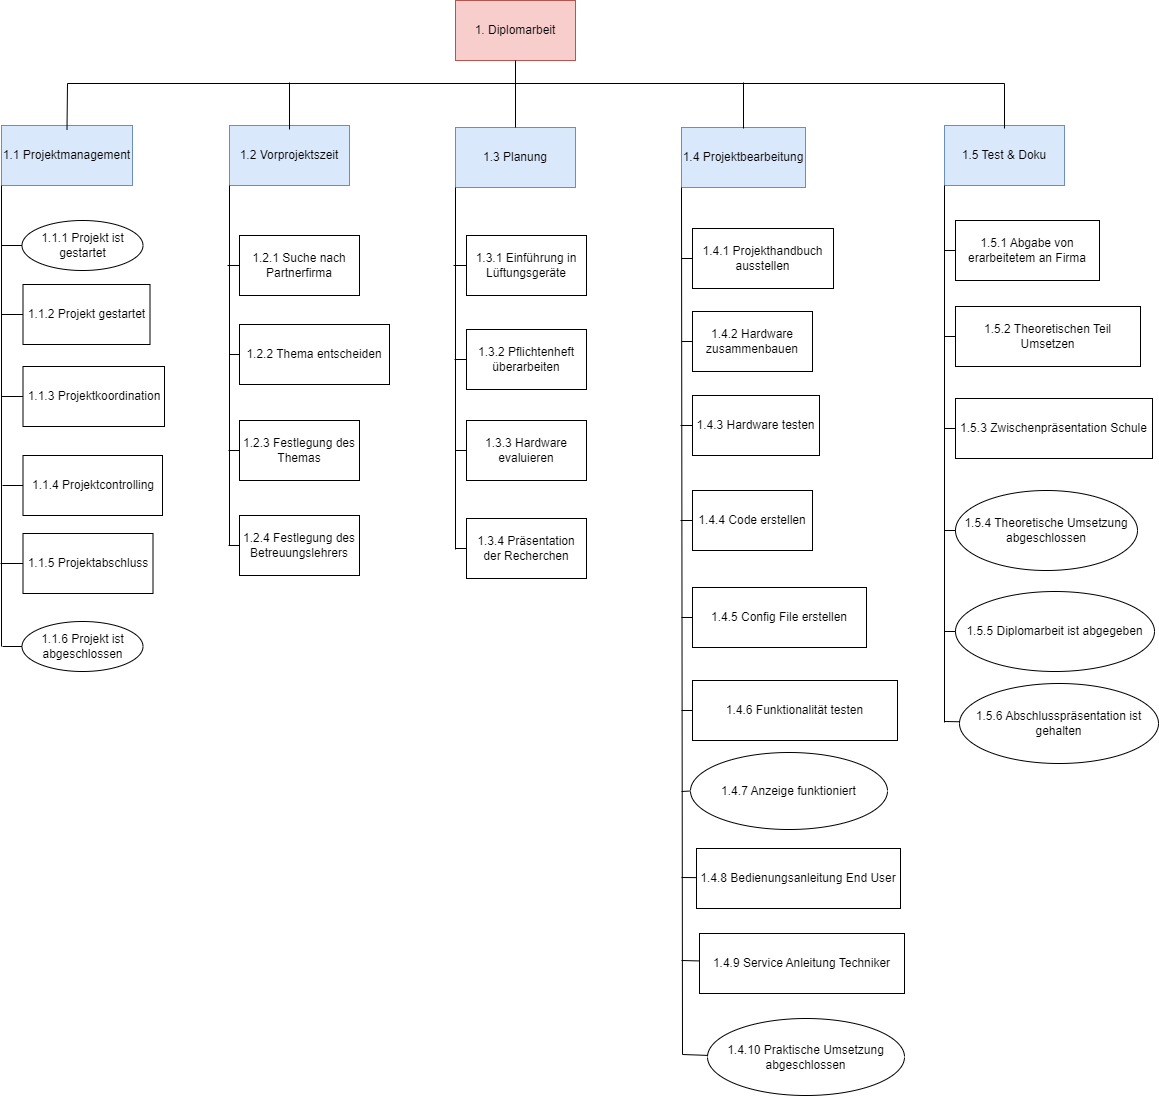
\includegraphics[width=1\linewidth]{Bilder/projektstrukturplan}
	\caption{Projektstukturplan}
	\label{fig:projektstrukturplan}
\end{figure}

\section{Objektstrukturplan}
Ein Objektstrukturplan wird am Anfang eines Projekts definiert. Dieser ist dafür zuständig, zu zeigen, welche Ergebnisse und Zwischenergebnisse im Projekt entstehen sollen. Dabei können diese sowohl materiell als auch immateriell sein. Der \enquote{OSP} hat keine zeitliche Abfolge und soll bei der Ausarbeitung des Projektstrukturplans helfen. Die Darstellung kann als Mindmap, aber auch als Baum- oder Listenstruktur erfolgen.

\section{Projektfunktionendiagramm}
Um die Zuständigkeiten in Projekten regeln zu können, existieren Projektfunktionendiagramme. Diese werden in Form einer Tabelle dargestellt und beinhalten alle Projektbeteiligten sowie alle Arbeitspakete. Bei den Beteiligten gelten folgende Kürzel:
\begin{itemize}
	\item \textbf{PAG} - Projektauftraggeber
	\item \textbf{PL} - Projektleiter
	\item \textbf{PTM} - Projektteammitglied
	\item \textbf{PM} - Projektmitarbeiter
\end{itemize}
Unter jedem Beteiligten sind die jeweiligen Funktionen dessen eintragbar, die bei der Ausführung des Arbeitspakets eingenommen wurde.
Bei den Funktionen gelten folgende Kürzel:
\begin{itemize}
	\item \textbf{D} - Durchführungsverantwortung
	\item \textbf{M} - Mitarbeit
	\item \textbf{I} - bekommt Informationen
\end{itemize}
Hier ist zu beachten, dass die Verantwortung eines Arbeitspakets nur durch eine Person übernommen werden kann \cite{prezi:o.J.}.

\section{Projektmeilensteinplan}
Zur Überprüfung, ob ein Projekt möglicherweise nicht zur richtigen Zeit beendet wird, kann der Meilensteinplan als Maßstab dienen. Er bildet die wichtigsten Ereignisse inklusive einer Deadline ab. So erhält man eine grobe Übersicht über Verzögerungen und es können Maßnahmen bei Bedarf ergriffen werden. Im Allgemeinen dient er aber auch der Mitarbeitermotivation bei Erreichen eines Zwischenziels oder Meilensteins \cite[vgl.][]{domendos:2016}. \\
In der folgenden Tabelle \ref{tab:meilensteinplan} befinden sich die Meilensteine inklusive deren Termine.

\begin{table}[H]
	\caption{Projektmeilensteinplan}
	\label{tab:meilensteinplan}
	\begin{tabular}{p{\dimexpr 0.10\textwidth-2\tabcolsep} | p{0.30\textwidth} | p{0.15\textwidth} | p{0.15\textwidth} | p{0.15\textwidth}}
		\toprule
		\textbf{PSP-Code} & \textbf{Meilenstein} & \textbf{Basis-Termine} & \textbf{Aktuelle Plantermine} & \textbf{Ist Termine} \\
		\midrule
		1.1.1 & M1 Projekt ist gestartet & 09.05.2023 & 09.05.2023 & 09.05.2023 \\
		\midrule
		1.4.7 & M2 Anzeige funktioniert & 02.08.2023 & 03.08.2023 & 03.08.2023 \\
		\midrule
		1.4.10 & M3 Praktische Umsetzung abgeschlossen & 03.08.2023 & 04.08.2023 & 04.08.2023 \\
		\midrule
		1.5.4 & M4 Theoretische Umsetzung abgeschlossen & 01.03.2024 & 01.03.2024 & 01.03.2024 \\
		\midrule
		1.5.5 & M5 Diplomarbeit ist abgegeben & 03.04.2024 & 03.04.2024 & 03.04.2024 \\
		\midrule
		1.5.6 & M6 Abschlusspräsentation ist gehalten & 13.06.2024 & 13.06.2024 & 13.06.2024 \\
		\midrule
		1.6 & M8 Projekt ist abgeschlossen & 13.06.2024 & 13.06.2024 & 13.06.2024 \\
		\bottomrule
	\end{tabular}
\end{table}


\section{Projektbalkenplan}
Während bei dem Meilensteinplan nur die Meilensteine abgebildet sind, werden im Projektbalkenplan alle Arbeitspakete und deren ungefähres Fälligkeitsdatum gezeigt. So hat man jederzeit einen Überblick über den terminlichen Status des Projektfortschritts. Daher ist der Projektbalkenplan oder \enquote{Gantt-Chart}  als zeitliche Ebene die erste Wahl, um einen umfassenden Überblick über den zeitlichen Status des Projektfortschritts zu behalten \cite[vgl.][]{domendos:2019}. \\
Auf der nächsten Seite befindet sich mit Abbildung \ref{fig:projektbalkenplan} der Balkenplan, der nach dem \enquote{PSP} aufgebaut ist.

\begin{landscape}
	\begin{figure}[H]
		\centering
		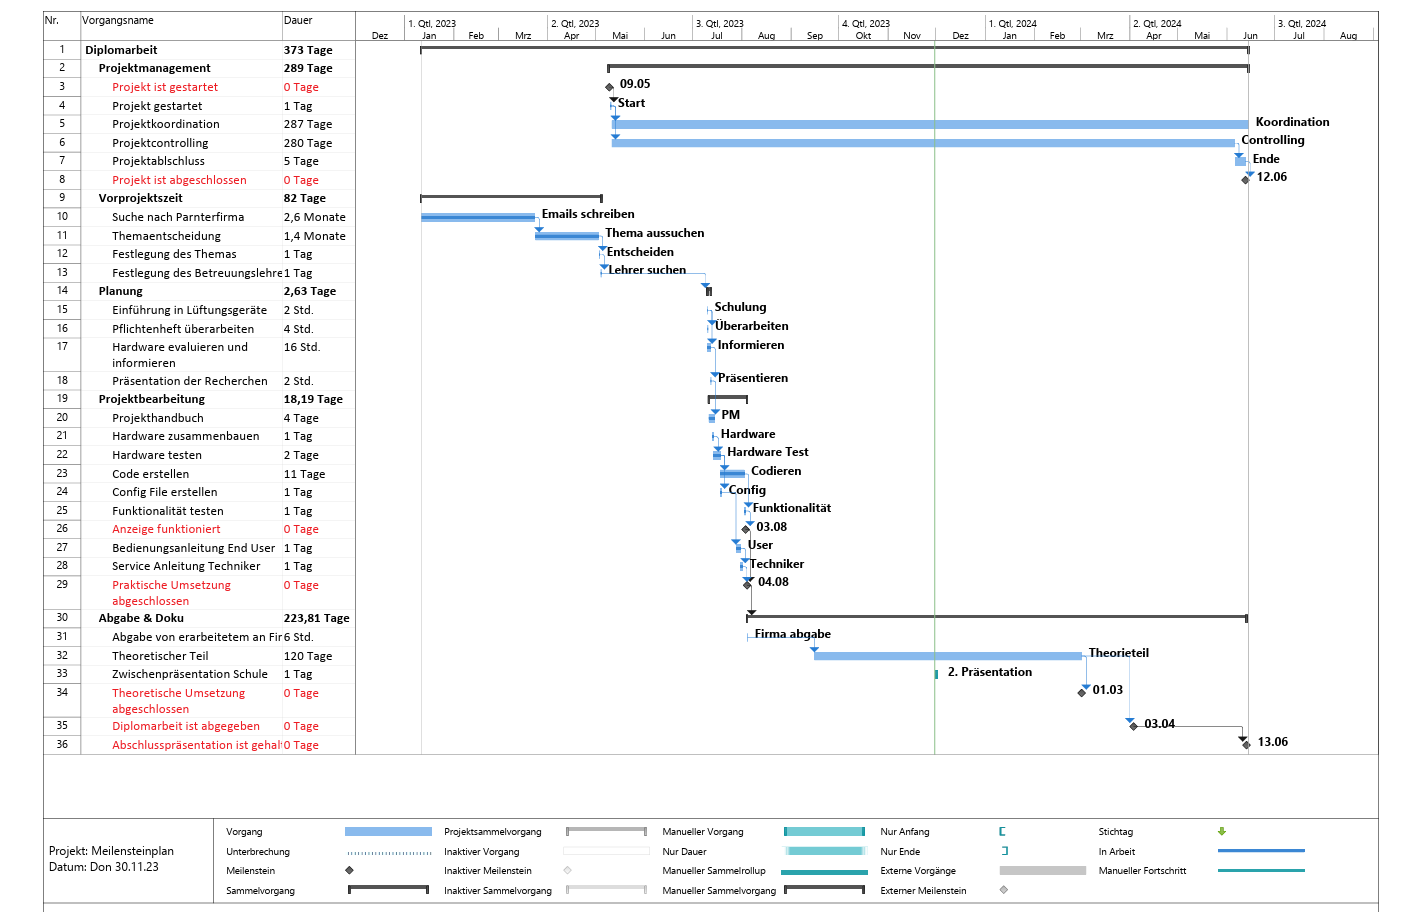
\includegraphics[width=1\linewidth]{Bilder/ganttchart}
		\caption{Projektbalkenplan}
		\label{fig:projektbalkenplan}
	\end{figure}
\end{landscape}

\section{Projektrisikoanalyse}
Risiken können in den meisten Fällen ein Projekt bedrohen. Daher ist es wichtig, Risiken im Vorhinein einzuschätzen und möglichst zu vermeiden. Manche Risiken können teilweise nicht umgangen werden, dafür, wenn das Risiko überwunden wurde, stärkt es das Projekt durch diese Herausforderung. Dennoch sollten diese immer zuvor bereits bemerkt werden, damit der Zeitaufwand mit einberechnet werden kann \cite{timetrackapp:2021}.

\begin{longtable}{p{\dimexpr 0.10\textwidth-2\tabcolsep} | p{0.20\textwidth} | p{0.20\textwidth} | p{0.10\textwidth} | p{0.10\textwidth} | p{0.20\textwidth}}
	\caption{Projektrisikoanalyse}
	\label{tab:risikoanalyse}
	\\ \toprule
	\textbf{PSP-Code} & \textbf{AP-Bezeichnung} & \textbf{Risiko-beschreibung} & \textbf{Prio} & \textbf{Verzö-gerung} & \textbf{korrektive Maßnahmen}
	\\ \midrule
	\endfirsthead
	\caption{Projektrisikoanalyse (Fortsetzung)}
	\\ \toprule
		\textbf{PSP-Code} & \textbf{AP-Bezeichnung} & \textbf{Risiko-beschreibung} & \textbf{Prio} & \textbf{Verzö-gerung} & \textbf{korrektive Maßnahmen}
	\\ \midrule
	\endhead
	%
	\midrule
	\multicolumn{6}{r}{{Auf nächster Seite weitergeführt}} 
	\\ \bottomrule
	\endfoot
	%
	\bottomrule
	\endlastfoot
	1.3.3 & Hardware evaluieren &  Für eine zu lange Zeit keine passenden Komponenten und keine Informationen für die Umsetzung finden & 1 & 1 Tag & Zu Beginn viel Zeit in das Recherchieren investieren und wichtige Informationen für später herausschreiben \\ \midrule
	1.4.2 & Hardware zusammenbauen & Möglicherweise passen die Teile nicht zusammen bzw. sind für andere Versionen des Chipsatzes gedacht & 2 & 3 Tage & Exzessiv auf die Informationen, die auf den Websites der Bauteile stehen, achten  \\ \midrule
	1.4.3 & Hardware testen & Defekte Komponente & 3 & 3 Tage & Neue Hardware muss bestellt werden \\ 
	1.4.4 & Code erstellen & Probleme bei der Programmierung der Modbus-Schnittstelle oder dem Anzeigen der Daten auf dem Display & 1 & 2 Tage & Vor dem Programmieren informieren und nach Libraries suchen, die die Einstellungen vereinfachen \\ \midrule
	1.4.4 & Code erstellen & Anforderungen von Arbeitgeber anders gewünscht als tatsächlich erledigt & 4 & 3 Tage & Klares absprechen, was im Projekt behandelt wird und auch wie \\ \midrule
	1.4.6 & Funktionalität testen & Mögliche weitere Anforderungen des Arbeitgebers nach eigentlicher Beendigung des Projekts  & 4 & 3-4 Tage & Durch ein klar definiertes und unterschriebenes Pflichtenheft müssen nur vorher besprochene Themen bearbeitet werden \\
\end{longtable}

\section{Projektkommunikationsstrukturen}
Neben der Erstellung von Plänen und Analysen ist der Projektleiter auch noch für die Projektkoordination und das Projektcontrolling zuständig. Dies gilt demnach natürlich auch für Meetings, die intern im Unternehmen für die Ausarbeitung der Diplomarbeit stattfanden. Die folgende Tabelle \ref{tab:strukturenplan} beinhaltet alle Treffen und Meetings inklusive Datum. \\
Stattgefunden hat alles bei der Firma Bösch in Lustenau, mit dem Projektansprechpartner Simon Köldorfer sowie allen Projektmitgliedern als Teilnehmern, abgesehen vom letzten Meeting, welches an der HTL Dornbirn stattfand mit Beisitz von Herrn Battlogg.

\begin{table}[H]
	\caption{Projektkommunikationsstrukturenplan}
	\label{tab:strukturenplan}
	\centering
	\begin{tabular}{p{\dimexpr 0.25\textwidth} | p{0.45\textwidth} | p{0.15\textwidth}}
		\toprule
		\textbf{Bezeichnung} & \textbf{Ziele, Inhalt} & \textbf{Termin} \\
		\midrule
			& • Diskussion Projektablauf & \\
		      Projektauftraggeber - &  • Besprechung Pflichtenheft  & 02.05.2023 \\
 			 Sitzung & • Freigabe Projektfortschrittsbericht & \\
 		\midrule
 			& • Fachspezifisches Personal kennen & \\
 		    Kennenlernen des & • Einführung in die Lüftungstechnik & 10.05.2023 \\
 			Personals	& • Ansprechperson bei Fragen & \\
 			& • Fragen zu Beginn geklärt & \\
 		\midrule
 			& •	Projektstatus & \\
 			& •	Hardware Möglichkeiten zeigen & \\
 		    Hardware -	& • Kosten, Ressourcen & 12.07.2023 \\ 
 			Präsentation & • Diskussion Problemstellungen & \\
 			& • Diskussion Lösungswege & \\
 			& •	Controlling Leistungsfortschritt & \\
 		\midrule
 			& •	Projektstatus & \\
 		Besprechung der & •	Design-Möglichkeiten & 27.07.2023 \\
 		anzuzeigenden Werte & •	Gewünschte Anzeigewerte besprechen & \\
 			& • Aufbau des Programms  & \\
 		\midrule
 			& •	Was ist abzugeben & \\
 		Weitere Schritte & • Vorhandene Probleme & 04.08.2023 \\
 			& •	Projektvorführung & \\
 			& •	Erklärung von Config Files & \\
 		\midrule
 			& •	Übergabe eines Gehäuseprototypen & \\
 		Tag der offenen Tür & • Gespräch über Möglichkeiten für die Präsentation & 09.11.2023 \\
 			& •	Besorgung von Hardware seitens Herrn Köldorfer& \\
		\bottomrule
	\end{tabular}
\end{table}

\ifoot{\leftmark}
\chapter{Tools}
%Tools (z.B. Latex, Figma, Shortbus)
Zur Ausarbeitung dieser Diplomarbeit wurden viele unterschiedliche Programme und Tools verwendet. Es folgt eine kurze Auflistung dieser:
\begin{itemize}
	\item \textbf{\LaTeX}: Zur Erstellung dieses Dokuments \textit{(weitere Erklärung folgt!!!!!)}
	\item \textbf{Word} und andere Editoren: Zur Erstellung von Notizen
	\item \textbf{Excel}: Um die Bewertungsmatrix der Hardwareauswahl zu erstellen
	\item \textbf{Onedrive}: Um die Notizen und Dokumente zu speichern und untereinander zugänglich zu machen.
	\item \textbf{Github}: Damit wurde der Programmcode verwaltet und gespeichert.
	\item \textbf{Discord und Whatsapp}: Zur internen Kommunikation zwischen den Teammitgliedern.
	\item \textbf{Outlook und Teams}: Zur Kommunikation mit der Firma und dem Betreuungslehrer.
	\item \textbf{Shortbus}: Es handelt sich hierbei um ein Programm, mit dem über eine grafische Oberfläche Modbus Register ausgelesen und gesetzt werden können (https://sourceforge.net/projects/shortbusmodbusscanner/). Damit konnte die Modbus Kommunikation getestet und die relevanten Register bestimmt werden.
	\item \textbf{Visual Studio Code und PyCharm}: Sind beides IDEs, mit denen das Python Programm der Anzeige entwickelt wurde.
	\item \textbf{Figma}: Siehe Kapitel \ref{figma_design} \nameref{figma_design}.
	\item \textbf{Zotero}: Es ist ein Literaturverwaltungsprogramm. Damit wurden Internetquellen gesammelt, damit sie in Latex importiert werden können.
\end{itemize}

\ifoot{\leftmark}
%gemeinsames Kapitel
\chapter{Zusammenfassung}


%\chapter{Beispiele}

In diesen Dateien finden Sie die Beispiele aus den youtube-Videos:

\url{https://www.youtube.com/playlist?list=PLwlC-XZXtzhg4fQiZQAsXIMSRW-iZtnTQ}

\section{section bsp}
\begin{figure}
	\centering
	
\includegraphics[width=0.4\linewidth]{Bilder/HTL_Dornbirn_Logo}
	\caption{HTL Dornbirn Logo (Quelle: \url{https://www.htldornbirn.at/})}
	\label{fig:htldornbirnlogo}
\end{figure}


\section{Beispiele aus dem Video zur Bachelorarbeit}
\setAuthor{\pezze}
\minisec{Tipps: Schreiben einer wissenschaftlichen Arbeit mit \LaTeX{}}
%
Generell stellt sich für uns das Problem, nun mit \LaTeX{} einfach und rasch eine wissenschaftliche Arbeit zu schreiben.
Den Inhalt nimmt uns \LaTeX{} leider nicht ab, dafür sind wir selbst verantwortlich.
Jedoch können wir uns bei \LaTeX{} auf einige Vorteile verlassen, die wir hier näher betrachten möchten.
Vorweg sei die konsistente Formatierung genannt.

Bevor wir diese Vorteile behandeln, beschäftigen wir uns mit generellen Anforderungen an wissenschaftliche Arbeiten.
Die Erstellung der Gliederung und des Aufbaus einer wissenschaftlichen Arbeit sind meist der erste Schritt für jede Autorin bzw. jeden Autor.
Danach beschäftigt uns der Inhalt, denn jeder dieser Punkte bei der Gliederung will auch mit sinnvollem Inhalt gefüllt sein.
Ausreichendes Datenmaterial (Zahlen, Daten, Fakten) sollte dann gesammelt werden oder sein.
Gute Bilder, ansprechende Diagramme und aussagekräftige Tabellen helfen jeder Leserin und jedem Leser bei der Erfassung des wissenschaftlichen Inhalts.

\minisec{Vorgehensweise: Gliederung und Aufbau}
%
Meist ist der erste Schritt einer wissenschaftlichen Arbeit die Erstellung einer Gliederung der Arbeit (entspricht meist grob dem Inhaltsverzeichnis).
Diese wird dann mit den Betreuern der Arbeit besprochen.
Die folgende Aufzählung zeigt so eine sinnvolle Gliederung einer wissenschaftlichen Arbeit:
%
\begin{itemize}
   \item Titelblatt / Deckblatt
   \item Kurzfassung (Deutsch)
   \item Abstract (Englisch)
   \item Inhaltsverzeichnis
\end{itemize}
\begin{enumerate}
   \item Einleitung
      \begin{enumerate}
         \item Problemstellung, Motivation
         \item Vorgehensweise
      \end{enumerate}
   \item Definitionen und Abgrenzungen (Grundlagen, Theorie, Vorarbeiten)
      \begin{enumerate}
         \item Begriff A
         \item Begriff B
         \item \dots
      \end{enumerate}
   \item Hauptteil (eigene Arbeiten inkl. Ergebnisse)
      \begin{enumerate}
         \item Argument 1
         \item Argument 2
         \item \dots
      \end{enumerate}
   \item Zusammenfassung und Schlussfolgerungen (Bewertung und Ausblick)
\end{enumerate}
\begin{itemize}
   \item Literaturverzeichnis
   \item optional Abkürzungsverzeichnis, weitere Verzeichnisse und Anhang
\end{itemize}
%

\minisec{Beispiele zur Typografie}
%
Den Arbeiten \enquote{typokurz -- Einige wichtige typografische Regeln}~(\textcite{Bier:09}) sowie \citetitle{Struckmann:07} (\textcite{Struckmann:07}) entnehmen wir direkt einige Tipps:
%
\begin{enumerate}
   \item \textsc{Auszeichnungen/Hervorhebungen von Text}
      \begin{description}
         \item[Kursive] Eigene Schriftform; \emph{integrierte} 
                      Auszeichnung, die erst auffällt, wenn man an die entsprechende Stelle kommt; 
                      im Normalfall für Auszeichungen im Text am besten geeignet.
         \item[Fette] Normalerweise in Textabschnitten zu vermeiden, viel zu
                      aufdringlich (\emph{aktive} Auszeichnung), zieht direkt die Aufmerksamkeit auf sich (daher für Nachschlagewerke sinnvoll); 
                      für Überschriften, Bezeichnungen von Tabellen und Abbildungen, für Teile von Aufzählungen und Verzeichnissen sowie Tabellenköpfen geeignet;  gelegentlich wird sie auch bei Literaturverweisen im Text verwendet.
         \item[Unterstreichung] Unbedingt zu vermeiden; Überbleibsel aus dem
                      Schreibmaschinenzeitalter, als es nur eine Schriftform auf der Schreibmaschine gab.
         \item[Kapitälchen] Auch nur verwenden, wenn man weiß, was man tut.
                      Das heißt, man (er-)kennt den Unterschied zwischen echten und falschen Kapitälchen.
      \end{description}
   \item \textsc{Striche}
      \begin{description}
         \item[Trennstrich, Bindestrich] wird auch \emph{Divis} genannt und ist
                      ein kurzer Strich. Er dient zur Silbentrennung bzw. zur Verbindung zusammengesetzter Wörter. 
                      In \LaTeX{}: \verb|-|.
         \item[Gedankenstrich] Halbgeviertstrich, länger als der Divis, steht
                      zwischen zwei Leerzeichen (außer in Verbindung mit einem Satzzeichen), \zB{} Ich hoffe sehr -- und das meine ich ganz ehrlich --, Sie bald zu treffen. 
                      In \LaTeX{}: \verb|--|.
         \item[Streckenstrich/Bis-Strich] Halbgeviertstrich ohne Leerzeichen
                      davor und dahinter (Ausnahme: in Verbindung mit Wörtern wird ein Leerzeichen verwendet), \zB{} Linz--Wien, 1--2 Telefonate, 25.9.--28.12., 325 v.Chr. -- 440 n.Chr. 
                      In \LaTeX{}: \verb|--|.
         \item[Auslassungsstrich] Der Halbgeviertstrich dient im Text auch als
                      Auslassungszeichen; in Tabellen sollte dafür ein Geviertstrich (---) verwendet werden, der die Breite von zwei Nullen hat.
                      In \LaTeX{}: \verb|---|.
      \end{description}
   \item \textsc{Absatzformatierung}: Absätze kann man auf zwei Arten
            voneinander trennen: \emph{Einzug} oder \emph{Abstand}. In Bezug auf wissenschaftliche Arbeiten gilt meist: Absätze werden durch einen Einzug von ca. \SI{4}{mm} gekennzeichnet. 
            Abschnitte werden durch einen Abstand von einer Leerzeile gekennzeichnet und im Unterschied zu Absätzen ohne Einzug gesetzt.
%
      \begin{labeling}[\dots]{Flattersatz }
          \item[Flattersatz] Dieser hat den großen Vorteil, dass die 
                      Wortzwischenräume immer gleich groß sind, was positiv für die Lesbarkeit ist. 
                      Andererseits wirkt der Flattersatz eher unruhig, vor allem bei schlechtem Zeilenumbruch.
          \item[Blocksatz] Ob man sich für oder gegen Blocksatz entscheidet, ist
                      abhängig von der Zeilenlänge, der Sprache, in der der Text verfasst wird, dem Mechanismus der Silbentrennung und dem Umbruchalgorithmus der verwendeten Software.
                      Will man für längere Zeilen Blocksatz verwenden, muss man sicherstellen, dass die Software gleichmäßige und enge Wortzwischenräume erzeugt; diese sollten innerhalb einer Zeile gleich groß sein und sich von jenen in der vorangehenden und nachfolgenden Zeile nicht deutlich unterscheiden. 
      \end{labeling}
%
   \item \textsc{Schriften}: Es ist sinnvoll, für längere Texte mit breiten 
            Zeilen eine Schrift mit Serifen und Strichstärkenunterschied zu verwenden.
            Die Serifen (Endstriche) unterstützen einerseits das Auge bei der Zeilenführung und beim Zeilenrücksprung.
            Andererseits führt der Strichstärkenunterschied zu eindeutigeren Wortbildern, was das Lesen sehr erleichtert.
            Am Bildschirm sind serifenlose Schriften bzw. solche ohneStrichstärkenunterschied in der Tat häufig besser zu lesen alsserifenbehaftete Schriften. 
            Daher ist der Vergleich der Schriften auf Papier wichtig.
   \item \textsc{Trennung von Abkürzungen}: Dies ist zu vermeiden. 
            Auch abgekürzte Einheiten sollen nach Möglichkeit nicht von den dazugehörigen Zahlen getrennt werden. 
            Dazu verwenden Sie die Tilde \~{} zwischen Zahl und Einheit (noch besser: die Befehle des \texttt{siunitx}-Pakets).
\end{enumerate}

\minisec{Zitate mit einer Fußnote}
%
\Name{Christian Wolf}%
\footnote{\Name{Christian Wolf} (1679-1754), Philosoph der deutschen Aufklärung und Professor der Mathematik}
%
beschreibt 1716 in seinem mathematischen Lexikon den Ingenieur folgendermaßen:
%
\begin{quotation}
\emph{
Ingenieur, architectus militaris, ein Kriegsbaumeister, ist eine Person, welche die Kriegsbaukunst oder Fortifikation übet und also nicht allein die Festungen anzugeben vermögend ist, sondern auch die Attacken bei deren Belagerung anzuordnen weiß.}
\end{quotation}

\minisec{Formeln mit Querverweis und Kurzbefehlen}
%
Schauen wir uns einige einfache Beispiele an.
In Gleichung~\eqref{Glg:Def_a1} sehen Sie eine Formel zur Berechnung einer Krümmungszahl der Eigenwertkurven bei Stabilitätsproblemen. 
%
\begin{equation}
   a_1=-\frac{1}{2}
        \frac{\mathbf{v}_1^T 
                    \frac{\tilde{\mathbf{K}}_{T},_{\xi\xi}\lambda,_{\xi} -
                          \tilde{\mathbf{K}}_{T},_{\xi}\lambda,_{\xi\xi}}
                         {\left(\lambda,_{\xi}\right)^3}
                         \mathbf{v}_1
             }
             {\mathbf{v}_1^T 
             \frac{\tilde{\mathbf{K}}_{T},_{\xi}}{\lambda,_{\xi}} 
             \mathbf{v}_1}
      = -\frac{1}{2\,\lambda,_{\xi}}
         \left(
               \frac{\vKTxxv}     % hier verwenden wir Kurzbefehle
                    {\vKTxv}      % hier ebenso
             - \frac{\lambda,_{\xi\xi}}{\lambda,_{\xi}}
         \right)
\label{Glg:Def_a1}
\end{equation}
%

\minisec{Mehrzeilige Formeln}
%
Für diese eignet sich vor allem die \texttt{align}-Umgebung (wie in Gleichung~\eqref{Glg:align}).
%
\begin{align}
   f(x) = & f(\bar x) + \frac{(x - \bar x)}{1!} \frac{df}{dx}
   \Bigg|_{x = \bar x} +
   \frac{(x - \bar x)^2}{2!} \frac{d^2 f}{d x^2} \Bigg|_{x = \bar x} +
   \dots + \nonumber \\
   \nonumber \\
          & +\frac{(x - \bar x)^n}{n!} \frac{d^n f}{d x^n} 
            \Bigg|_{x = \bar x} +
            \frac{(x - \bar x)^{n+1}}{(n + 1)!}
            \frac{d^{(n + 1)} f}{d x^{(n + 1)}} 
            \Bigg|_{\bar x + \vartheta (x - \bar x)} \, ,
\label{Glg:align}
\end{align}
%
wobei $0 < \vartheta < 1$ ist.
%
\begin{align}
   M(x) & =  M(\bar x) &  A & = \SI{10,3}{kN}  &  M_{\max} & = \SI{85,2}{kNm}
\nonumber \\
   V(x) & = V(\bar x)  &  B & = \SI{18,7}{kN}  &  V_{\max} & = \SI{20,2}{kN}
\label{Glg:align2}
\end{align}

\newpage
\section{Beispiele aus dem Video zur DA und Diss}
\setAuthor{\schneider}
\minisec{Zwei Abbildungen nebeneinander}
%
\texttt{Abbildungen} fallen unter \emph{floating objects} und werden in der \texttt{figure}-Umgebung in den Text eingebunden.
Für mehrere Bilder in einer Abbildung mit jeweils eigener Beschriftung können wir die \texttt{subfigure}-Umgebung verwenden (siehe Abb.~\ref{fig:bsp-subfigure})
%
Abb.~\ref{fig:xkcd-citogenesis} zeigt ein Problem des Zitierens aus Wikipedia. 
Da manche Menschen alles glauben, was in Wikipedia geschrieben steht, stellt dieser Comik aus \url{https://xkcd.com} die Glaubwürdigkeit zumindest ein bisschen in Frage.
Eine Erklärung dazu befindet sich auf \url{https://www.explainxkcd.com/wiki/index.php/978:_Citogenesis}.
Abb.~\ref{fig:logo-fakultät} zeigt das Logo unserer Fakultät.
%
\begin{figure}[ht]
  \begin{subfigure}[t]{0.50\textwidth}
   \centering
   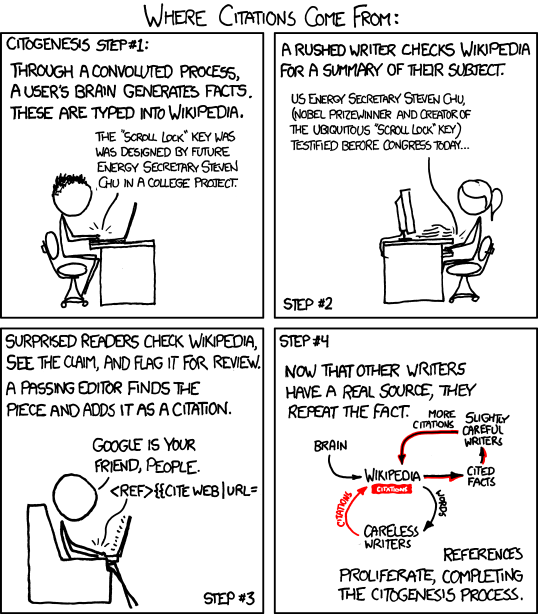
\includegraphics[width=7cm]{citogenesis}
   \caption[Zitierproblematik]{Ein Glaubwürdigkeitsproblem mancher Artikel in Wikipedia (Quelle: \url{https://xkcd.com/978/})    \label{fig:xkcd-citogenesis}}
  \end{subfigure}
\hfill
  \begin{subfigure}[t]{0.45\textwidth}
   \centering
   \caption{Logo der Fakultät für Bau- und Umweltingenieurwesen der TU Wien \label{fig:logo-fakultät}}
  \end{subfigure}
\caption{Beispiel einer \texttt{subfigure}-Umgebung \label{fig:bsp-subfigure}}
\end{figure}
%


\minisec{Matrix-Schreibweise}
%
Die Steifigkeitsmatrix sowie die Nachgiebigkeitsmatrix des Materials sind mit Bezug auf die Materialhauptrichtungen $L$-$R$-$T$ gegeben (siehe~\eqref{Glg:sigma} bis \eqref{Glg:D-matrix}).

Gesucht ist der Verzerrungstensor $\varepsilon$ im globalen Koordinatensystem $X,Y,Z$ sowie die Koordinaten der Eckpunkte in der verformten Lage (angegeben in [\si{mm}] auf 3~Dezimalstellen) unter der Annahme einer linearisierten Elastizitätstheorie.

\begin{equation}
\boldsymbol{\sigma}
=
\left(
   \begin{array}{c}
      \sigma_{xx} \\
      \sigma_{yy} \\
      \sigma_{zz} \\
      \sigma_{xy} \\
      \sigma_{yz} \\
      \sigma_{zx} \\
   \end{array}
\right)
=
\left(
   \begin{array}{c}
      1x{,}y \\
      1{,}xy \\
      2{,}xy \\
      3{,}xy \\
      0      \\
      0      \\
   \end{array}
\right)
\si{N/mm^2}
\label{Glg:sigma}
\end{equation}

\begin{equation}
\textbf{C}_{(LRT)}
=
\left(
\begin{array}{rrrccc}
\num{15500} & 489 & 274 & 0   & 0  & 0  \\
      & 844 & 162 & 0   & 0  & 0  \\
      &     & 632 & 0   & 0  & 0  \\
      &     &     & 700 & 0  & 0  \\
      &     &     &     & 60 & 0  \\
   \multicolumn{2}{l}{\text{symm.}}  
            &     &     &    & 650 \\
\end{array}
\right)
%
\cdot
%
\left(
   \begin{array}{c}
      \epsilon_{xx} \\
      \epsilon_{yy} \\
      \epsilon_{zz} \\
      \epsilon_{xy} \\
      \epsilon_{yz} \\
      \epsilon_{zx} \\
   \end{array}
\right)
=
\left(
   \begin{array}{r}
      \num{12,70} \\
      \num{1,27}  \\
      \num{2,27}  \\
      \num{3,27}  \\
      \multicolumn{1}{c}{0}     \\
      \multicolumn{1}{c}{0}     \\
   \end{array}
\right)
\label{Glg:C-matrix}
\end{equation}

\begin{equation}
\textbf{D}_{(LRT)}
=
\left(
   \begin{array}{rrrccc}
\num{6,595} &  \num{-3,441} &  \num{-1,977} &  0  &  0  & 0 \\
            & \num{126,411} & \num{-30,911} &  0  &  0  & 0 \\
            &               & \num{167,008} &  0  &  0  & 0 \\
            &               &               & \num{142,857} &  0  &  0  \\
            &               &               &    & \num{1666,667}  &  0  \\
   \multicolumn{2}{l}{\text{symm.}} &       &    &      & \num{153,846}  \\
\end{array}
\right)
\cdot \SI{e-5}{mm^2/N}
\label{Glg:D-matrix}
\end{equation}



\minisec{Beispiel für xfrac-Paket}
%
Dieses Paket verwendet den Befehl \textbackslash{}sfrac\{\}\{\} im Text
\sfrac{3}{4} oder in einer Formel $\sfrac{3}{4}$.

\minisec{Beispiele für den Einsatz des siunitx-packages}
Eine Verwendungsmöglichkeit ist die richtige Anzeige von Zahlen:
%
\begin{itemize} 
  \item als Einzelzahl: \num{12345678,9202}
  \item als Bereich von Zahlen: \numrange{12,3}{14,7} 
  \item als Liste von Zahlen: 
                      \numlist[list-final-separator={ und }]{12,3;13,5;14,7}
\end{itemize}
%
oder die richtige Darstellung von Einheiten (unabhängig ob im Paragraph- oder Math-Modus):
%
\begin{itemize} 
  \item Paragraphmodus: \si{\kilo\newton\per\meter}, \si{kN/m^2}
  \item Mathematikmodus:  $\si{\kilo\newton\per\meter}$, $\si{kN/m^2}$
\end{itemize}
%
oder die richtige Darstellung von Zahlen mit Einheiten:
%
\begin{itemize} 
  \item als Einzelzahl: \SI{12345678,92}{kNm}
  \item als Winkel: \ang{10}, \ang{12.3} oder \ang{12;3;5}
  \item als Bereich von Zahlen: \SIrange{12,3}{14,7}{\%} oder 
          \SIrange[range-units = single]{12,3}{14,7}{\%}
  \item als Liste von Zahlen: 
        \SIlist[list-final-separator={ und }]{12,3;13,5;14,7}{\kilogram/m^2}
\end{itemize}
%

\minisec{Beipiele für Abkürzungen samt zugehörigem Verzeichnis}

Das Programm \ac{rlt} wurde in Zusammenarbeit mit der \ac{obv} erstellt, berücksichtigt die deutsche \ac{abbv} -- von mehreren \aclp{abbv} -- und berechnet \ac{lzk}.

Nochmals:
Das Programm LZKB wurde in Zusammenarbeit mit der \ac{obv} erstellt, berücksichtigt die deutsche \ac{abbv} -- von mehreren \acp{abbv} -- und berechnet \ac{lzk}.

\printacronyms[name=Abkürzungen]



\minisec{Beispiel für den Einsatz des tabularx-packages}
Dieses Paket bietet die Möglichkeit der automatischen Anpassung der Spaltenbreite auf eine Gesamtbreite der Tabelle (siehe Tab.~\ref{tab:test}).


\begin{table}[h]
\caption{Ergebnisse der schriftlichen Prüfung \label{tab:test}}
   \begin{tabularx}{\textwidth}{@{}lccX@{}}
   \toprule
   Name & Entwurf     & Pläne       & Anmerkung    \\
   \midrule
   Mayer    & \SI{60}{\%} & \SI{60}{\%} & 
      Funktionalle Umsetzung mit hinreichender Routine. Konstruktive Darstellung speziell im Dachbereich nicht nachvollziehbar. \\
   Müller   & \SI{20}{\%} & \SI{30}{\%} & 
      In allen Teilbereichen sehr detailierte Konzeption, allerdings fehlt die planliche Umsetzung, sodass aufgrund des fehlenden Informationsgehalts keine positive Beurteilung möglich ist. \\
   Schmidt  & \SI{90}{\%} & \SI{90}{\%} & 
      In allen Prüfungsabschnitte routinierte Darstellung und planliche Umsetzung. Die Nachvollziehbarkeit ist in allen Teilabschnitten gegeben. \\
   \bottomrule
   \end{tabularx}
\end{table}




\minisec{Beispiel für den Einsatz der longtable- und multirow-packages}

\begin{longtable}{@{}l*{3}{S[table-format=2.2]}@{}}
\caption{Messwerte der bauphysikalischen Untersuchung \label{tab:bauphysik}}
\\ \toprule
Datum & {Mittel [\si{\degreeCelsius}]} & {Min [\si{\degreeCelsius}]} & {Max [\si{\degreeCelsius}]}
\\ \midrule
\endfirsthead
\caption{Messwerte der bauphysikalischen Untersuchung (Fortsetzung)}
\\ \toprule
Datum & {Mittel [\si{\degreeCelsius}]} & {Min [\si{\degreeCelsius}]} & {Max [\si{\degreeCelsius}]}
\\ \midrule
\endhead
%
  \midrule
  \multicolumn{4}{r}{{Continued on next page}} 
  \\ \bottomrule
\endfoot
%
  \bottomrule
\endlastfoot
06-Jul-2016 & 24,6 & 20,9 & 25,0 \\
07-Jul-2016 & 24,82 & 24,50 & 25,30 \\
08-Jul-2016 & 24,58 & 24,30 & 25,10 \\
09-Jul-2016 & 24,58 & 24,40 & 24,80 \\
10-Jul-2016 & 24,53 & 24,40 & 24,90 \\
11-Jul-2016 & 24,55 & 24,20 & 25,00 \\
12-Jul-2016 & 24,55 & 24,40 & 24,70 \\
13-Jul-2016 & 24,55 & 24,40 & 24,70 \\
14-Jul-2016 & 25,02 & 24,50 & 25,40 \\
15-Jul-2016 & 25,22 & 24,80 & 25,50 \\
16-Jul-2016 & 25,45 & 25,30 & 25,70 \\
17-Jul-2016 & 25,35 & 24,80 & 25,70 \\
18-Jul-2016 & 25,29 & 24,80 & 25,70 \\
19-Jul-2016 & 24,83 & 24,60 & 25,10 \\
20-Jul-2016 & 24,73 & 24,60 & 25,00 \\
21-Jul-2016 & 24,68 & 24,50 & 24,90 \\
22-Jul-2016 & 24,70 & 24,60 & 25,00 \\
23-Jul-2016 & 24,72 & 24,60 & 25,00 \\
24-Jul-2016 & 24,81 & 24,60 & 25,00 \\
25-Jul-2016 & 24,74 & 24,50 & 25,00 \\
26-Jul-2016 & 24,70 & 24,60 & 24,80 \\
27-Jul-2016 & 24,72 & 24,50 & 25,00 \\
28-Jul-2016 & 24,66 & 24,50 & 24,90 \\
29-Jul-2016 & 24,66 & 24,50 & 24,80 \\
30-Jul-2016 & 24,69 & 24,60 & 24,80 \\
31-Jul-2016 & 24,77 & 24,70 & 25,00 \\
01-Aug-2016 & 24,72 & 24,40 & 25,00 \\
02-Aug-2016 & 24,64 & 24,50 & 24,90 \\
03-Aug-2016 & 24,73 & 24,60 & 25,00 \\
04-Aug-2016 & 24,74 & 24,60 & 24,80 \\
05-Aug-2016 & 24,76 & 24,60 & 25,20 \\
06-Aug-2016 & 25,30 & 24,80 & 25,70 \\
07-Aug-2016 & 25,10 & 24,70 & 25,60 \\
08-Aug-2016 & 25,06 & 24,80 & 25,50 \\
09-Aug-2016 & 24,89 & 24,70 & 25,20 \\
10-Aug-2016 & 25,52 & 25,00 & 25,80 \\
11-Aug-2016 & 25,60 & 25,30 & 25,80 \\
12-Aug-2016 & 25,81 & 25,60 & 26,00 \\
13-Aug-2016 & 25,95 & 25,50 & 26,30 \\
14-Aug-2016 & 25,79 & 25,40 & 26,30 \\
15-Aug-2016 & 25,47 & 25,20 & 25,90 \\
16-Aug-2016 & 25,36 & 25,10 & 25,90 \\
17-Aug-2016 & 25,33 & 25,10 & 25,80 \\
18-Aug-2016 & 25,42 & 25,00 & 25,90 \\
19-Aug-2016 & 25,36 & 25,00 & 25,70 \\
20-Aug-2016 & 25,37 & 25,00 & 25,80 \\
21-Aug-2016 & 25,38 & 25,10 & 25,70 \\
22-Aug-2016 & 25,88 & 25,60 & 26,20 \\
23-Aug-2016 & 25,85 & 25,10 & 26,70 \\
24-Aug-2016 & 25,10 & 24,80 & 26,30 \\
25-Aug-2016 & 25,22 & 24,80 & 25,70 \\
26-Aug-2016 & 24,91 & 24,70 & 25,30 \\
27-Aug-2016 & 24,75 & 24,60 & 25,00 \\
28-Aug-2016 & 24,74 & 24,60 & 25,00 \\
29-Aug-2016 & 24,76 & 24,50 & 25,00 \\
30-Aug-2016 & 24,77 & 24,60 & 25,10 \\
31-Aug-2016 & 24,87 & 24,60 & 25,30 \\
01-Sep-2016 & 24,97 & 24,60 & 25,60 \\
02-Sep-2016 & 24,78 & 24,60 & 25,10 \\
03-Sep-2016 & 24,95 & 24,70 & 25,40 \\
04-Sep-2016 & 24,91 & 24,70 & 25,20 \\
05-Sep-2016 & 25,21 & 24,80 & 25,70 \\
06-Sep-2016 & 25,81 & 25,40 & 26,40 \\
07-Sep-2016 & 26,01 & 25,50 & 26,50 \\
08-Sep-2016 & 25,66 & 25,30 & 26,30 \\
09-Sep-2016 & 25,29 & 25,10 & 25,40 \\
10-Sep-2016 & 25,20 & 25,10 & 25,30 \\
11-Sep-2016 & 25,19 & 25,00 & 25,40 \\
12-Sep-2016 & 25,08 & 24,80 & 25,40 \\
13-Sep-2016 & 24,92 & 24,80 & 25,00 \\
14-Sep-2016 & 24,81 & 24,60 & 24,90 \\
15-Sep-2016 & 24,76 & 24,50 & 25,00 \\
16-Sep-2016 & 24,94 & 24,80 & 25,20 \\
17-Sep-2016 & 25,04 & 24,80 & 25,50 \\
18-Sep-2016 & 25,44 & 25,10 & 25,80 \\
19-Sep-2016 & 25,70 & 25,40 & 26,00 \\
20-Sep-2016 & 25,85 & 25,70 & 26,10 \\
21-Sep-2016 & 25,92 & 25,70 & 26,20 \\
22-Sep-2016 & 25,94 & 25,70 & 26,20 \\
23-Sep-2016 & 25,87 & 25,50 & 26,30 \\
24-Sep-2016 & 26,01 & 25,60 & 26,40 \\
\multirow{3}{*}{25--27-Sep-2016} 
            & 26,00 & 25,60 & 26,30 \\
            & 26,19 & 25,70 & 26,50 \\
            & 26,19 & 25,50 & 26,50 \\
\end{longtable}

\minisec{Beispiel für den Einsatz des threeparttable-packages}

\begin{table}[htpb]
  \centering
  \caption{Beispiel für einen threeparttable}
  \label{tab:near_optimal}
  \begin{threeparttable}
    \begin{tabular}{@{}l|lllll@{}}\toprule
      Location\tnote{1}             & Beam 1    & Beam 2    & Beam 3    & Beam 4    & Beam 5    \\ \midrule
      1                             & 16$^\ast$ & 21        & 28        & 32        & 36$^\ast$ \\
      2                             & 14$^\ast$ & 33        & 47        & 37$^\ast$ & 35$^\ast$ \\ \midrule
      Deflection [$10^{-5}\si{mm}$] & $4.4753$  & $4.4575$  & $4.5067$  & $4.5076$  & $4.4642$  \\
    \bottomrule\end{tabular}
    \begin{tablenotes}
    \item[] Lamella IDs marked with an asterisk are flipped
    \item[1] The location is defined from top to bottom of the beam.
    \end{tablenotes}
  \end{threeparttable}
\end{table}







\ifoot{\leftmark}

\phantomsection
\clearpage
\addcontentsline{toc}{chapter}{Literatur}
\printbibliography

\phantomsection
\clearpage
\addcontentsline{toc}{chapter}{Abbildungsverzeichnis}
{\renewcommand{\addvspace}[1]{} \listoffigures}

\phantomsection
\clearpage
\addcontentsline{toc}{chapter}{Tabellenverzeichnis}
{\renewcommand{\addvspace}[1]{} \listoftables}

\printglossary[nonumberlist]

\phantomsection
\clearpage
\addcontentsline{toc}{chapter}{Abkürzungen}
\printacronyms[name=Abkürzungen]

\appendix

\printglossaries
\printbibliography
\listoffigures
\listoftables
\printacronyms[name=Abkürzungen]

\addchap{JSON Konfigurationsdateien Beispiele}
\paragraph{Beispiel einer Sensor-Konfigurationsdatei \enquote{sensors.json}:}
\begin{jsoncode}
{
	[
		{
			"type": "NI1000",
			"unit": "°C"
		},
		{
			"type": "NTC10K",
			"unit": "°C"
		},
		{
			"type": "PT1000",
			"unit": "°C"
		},
		{
			"type": "0-10V",
			"unit": "mV"
		},
		{
			"type": "LG-NI1000",
			"unit": "°C"
		},
		{
			"type": "standardQBM",
			"unit": "Pa"
		},
		{
			"type": "RPMmax",
			"unit": "1/min"
		}
	]
}
\end{jsoncode}

\paragraph{Beispiel der Geräte-Konfigurationsdateien}
\textbf{\enquote{QBM97XX.json}:}
\begin{jsoncode}
{
	"ports": [
		{
			"port": "P1",
			"register": 5,
			"function_code": 3,
			"units": [
				{
					"unit": "Pa",
					"scaling": 1
				}
			]
		},
		{
			"port": "P2",
			"register": 7,
			"function_code": 3,
			"units": [
				{
					"unit": "Pa",
					"scaling": 1
				}
			]
		},
		{
			"port": "AI1",
			"register": 9,
			"function_code": 3,
			"units": [
				{
					"unit": "°C",
					"scaling": 0.1
				},
				{
					"unit": "mV",
					"scaling": 1
				}
			]
		},
		{
			"port": "AI2",
			"register": 11,
			"function_code": 3,
			"units": [
				{
					"unit": "°C",
					"scaling": 0.1
				},
				{
					"unit": "mV",
					"scaling": 1
				}
			]
		},
		{
			"port": "AO1",
			"register": 27,
			"function_code": 3
		},
		{
			"port": "AO2",
			"register": 57,
			"function_code": 3
		}
	]
}
\end{jsoncode}

\textbf{\enquote{EBM.json}:}
\begin{jsoncode}
{
	"ports": [
		{
			"port": "RPMreal",
			"register": 53264,
			"function_code": 4
		},
		{
			"port": "RPMtarget",
			"register": 53249,
			"function_code": 3
		},
		{
			"port": "RPMmax",
			"register": 53529,
			"function_code": 3,
			"units": [
				{
					"unit": "1/min",
					"scaling": 1
				}
			]
		},
		{
			"port": "Power",
			"register": 53281,
			"function_code": 4
		},
		{
			"port": "Uz",
			"register": 53664,
			"function_code": 3
		},
		{
			"port": "Iz",
			"register": 53665,
			"function_code": 3
		},
		{
			"port": "Volume",
			"register": 53269,
			"function_code": 3
		},
		{
			"port": "EngStatus",
			"register": 53270,
			"function_code": 3
		}
	]
}
\end{jsoncode}


\paragraph{Beispiel einer Haupt-Konfigurationsdatei \enquote{main\_config\_file.json}:}
\begin{jsoncode}
[
	{
		"pages": [
			{
				"title": "Temperaturen",
				"sources": [
					{
						"port": [ {"QBM1": "AI1"} ],
						"description": "AUL. Temperatur"
					},
					{
						"port": [ {"QBM1": "AI2"} ],
						"description": "ZUL. Temperatur"
					},
					{
						"port": [
							{"QBM1": "AI1"},
							{"QBM1": "AI2"},
							{"QBM1": "AI1"}
						],
						"description": "Wärmerückgewinnungsgrad",
						"python_function": "calc_wrg"
					}
				]
			},
			{
				"title": "Allgemein",
				"sources": [
					{
						"port": [ {"QBM1": "P1"} ],
						"description": "ZUL. Filter Druckdifferenz"
					},
					{
						"port": [ {"QBM1": "P2"} ],
						"description": "ABL. Filter Druckdifferenz"
					},
					{
						"port": [ {"QBM1": "AI1"} ],
						"description": "Frostschutz Temperatur"
					},
					{
						"port": [ {"QBM1": "AO1"} ],
						"description": "AUL. Klappe",
						"python_function": "flap_position"
					},
					{
						"port": [ {"QBM1": "AO2"} ],
						"description": "WRG. Relais",
						"python_function": "relay_position",
						"additional_info": {"switching_voltage": 8}
					}
				]
			},
			{
				"title": "Ventilator Abluft",
				"sources": [
					{
						"port": [
							{"EBM1": "RPMreal"},
							{"EBM1": "RPMmax"}
						],
						"description": "Drehzahl Istwert",
						"python_function": "calc_rpm"
					},
					{
						"port": [
							{"EBM1": "RPMtarget"},
							{"EBM1": "RPMmax"}
						],
						"description": "Drehzahl Sollwert",
						"python_function": "calc_rpm"
					},
					{
						"port": [
							{"EBM1": "Power"},
							{"EBM1": "Uz"},
							{"EBM1": "Iz"}
						],
						"description": "Leistung",
						"python_function": "calc_power"
					},
					{
						"port": [ {"QBM1": "P1"} ],
						"description": "Volumen",
						"python_function": "calc_volume",
						"additional_info": {"k-faktor": 116}
					},
					{
						"port": [ {"EBM1": "EngStatus"} ],
						"description": "Motorstatus",
						"python_function": "eng_status"
					}
				]
			}
		],
		"devices": [
			{
				"device": "QBM97XX",
				"id": "QBM1",
				"baud_rate": 19200,
				"mbaddress": 41,
				"parity": "even",
				"stop_bits": 1,
				"zero_based": false,
				"sensors": [
					{
						"port": "P1",
						"type": "standardQBM"
					},
					{
						"port": "P2",
						"type": "standardQBM"
					},
					{
						"port": "AI1",
						"type": "LG-NI1000"
					},
					{
						"port": "AI2",
						"type": "LG-NI1000"
					}
				]
			},
			{
				"device": "EBM",
				"id": "EBM1",
				"baud_rate": 19200,
				"mbaddress": 33,
				"parity": "even",
				"stop_bits": 1,
				"zero_based": true
			}
		]
	}
]
\end{jsoncode}

\end{document}
